\documentclass[twoside]{book}

% Packages required by doxygen
\usepackage{fixltx2e}
\usepackage{calc}
\usepackage{doxygen}
\usepackage[export]{adjustbox} % also loads graphicx
\usepackage{graphicx}
\usepackage[utf8]{inputenc}
\usepackage{makeidx}
\usepackage{multicol}
\usepackage{multirow}
\PassOptionsToPackage{warn}{textcomp}
\usepackage{textcomp}
\usepackage[nointegrals]{wasysym}
\usepackage[table]{xcolor}

% Font selection
\usepackage[T1]{fontenc}
\usepackage[scaled=.90]{helvet}
\usepackage{courier}
\usepackage{amssymb}
\usepackage{sectsty}
\renewcommand{\familydefault}{\sfdefault}
\allsectionsfont{%
  \fontseries{bc}\selectfont%
  \color{darkgray}%
}
\renewcommand{\DoxyLabelFont}{%
  \fontseries{bc}\selectfont%
  \color{darkgray}%
}
\newcommand{\+}{\discretionary{\mbox{\scriptsize$\hookleftarrow$}}{}{}}

% Page & text layout
\usepackage{geometry}
\geometry{%
  a4paper,%
  top=2.5cm,%
  bottom=2.5cm,%
  left=2.5cm,%
  right=2.5cm%
}
\tolerance=750
\hfuzz=15pt
\hbadness=750
\setlength{\emergencystretch}{15pt}
\setlength{\parindent}{0cm}
\setlength{\parskip}{3ex plus 2ex minus 2ex}
\makeatletter
\renewcommand{\paragraph}{%
  \@startsection{paragraph}{4}{0ex}{-1.0ex}{1.0ex}{%
    \normalfont\normalsize\bfseries\SS@parafont%
  }%
}
\renewcommand{\subparagraph}{%
  \@startsection{subparagraph}{5}{0ex}{-1.0ex}{1.0ex}{%
    \normalfont\normalsize\bfseries\SS@subparafont%
  }%
}
\makeatother

% Headers & footers
\usepackage{fancyhdr}
\pagestyle{fancyplain}
\fancyhead[LE]{\fancyplain{}{\bfseries\thepage}}
\fancyhead[CE]{\fancyplain{}{}}
\fancyhead[RE]{\fancyplain{}{\bfseries\leftmark}}
\fancyhead[LO]{\fancyplain{}{\bfseries\rightmark}}
\fancyhead[CO]{\fancyplain{}{}}
\fancyhead[RO]{\fancyplain{}{\bfseries\thepage}}
\fancyfoot[LE]{\fancyplain{}{}}
\fancyfoot[CE]{\fancyplain{}{}}
\fancyfoot[RE]{\fancyplain{}{\bfseries\scriptsize Generated by Doxygen }}
\fancyfoot[LO]{\fancyplain{}{\bfseries\scriptsize Generated by Doxygen }}
\fancyfoot[CO]{\fancyplain{}{}}
\fancyfoot[RO]{\fancyplain{}{}}
\renewcommand{\footrulewidth}{0.4pt}
\renewcommand{\chaptermark}[1]{%
  \markboth{#1}{}%
}
\renewcommand{\sectionmark}[1]{%
  \markright{\thesection\ #1}%
}

% Indices & bibliography
\usepackage{natbib}
\usepackage[titles]{tocloft}
\setcounter{tocdepth}{3}
\setcounter{secnumdepth}{5}
\makeindex

% Hyperlinks (required, but should be loaded last)
\usepackage{ifpdf}
\ifpdf
  \usepackage[pdftex,pagebackref=true]{hyperref}
\else
  \usepackage[ps2pdf,pagebackref=true]{hyperref}
\fi
\hypersetup{%
  colorlinks=true,%
  linkcolor=blue,%
  citecolor=blue,%
  unicode%
}

% Custom commands
\newcommand{\clearemptydoublepage}{%
  \newpage{\pagestyle{empty}\cleardoublepage}%
}

\usepackage{caption}
\captionsetup{labelsep=space,justification=centering,font={bf},singlelinecheck=off,skip=4pt,position=top}

%===== C O N T E N T S =====

\begin{document}

% Titlepage & ToC
\hypersetup{pageanchor=false,
             bookmarksnumbered=true,
             pdfencoding=unicode
            }
\pagenumbering{alph}
\begin{titlepage}
\vspace*{7cm}
\begin{center}%
{\Large Flood it \\[1ex]\large Flood It by Olivier Cordier }\\
\vspace*{1cm}
{\large Generated by Doxygen 1.8.12}\\
\end{center}
\end{titlepage}
\clearemptydoublepage
\pagenumbering{roman}
\tableofcontents
\clearemptydoublepage
\pagenumbering{arabic}
\hypersetup{pageanchor=true}

%--- Begin generated contents ---
\chapter{Namespace Index}
\section{Namespace List}
Here is a list of all namespaces with brief descriptions\+:\begin{DoxyCompactList}
\item\contentsline{section}{\hyperlink{namespaceoli}{oli} }{\pageref{namespaceoli}}{}
\item\contentsline{section}{\hyperlink{namespace_ui}{Ui} }{\pageref{namespace_ui}}{}
\end{DoxyCompactList}

\chapter{Hierarchical Index}
\section{Class Hierarchy}
This inheritance list is sorted roughly, but not completely, alphabetically\+:\begin{DoxyCompactList}
\item \contentsline{section}{oli\+:\+:Board}{\pageref{classoli_1_1_board}}{}
\item \contentsline{section}{oli\+:\+:Color\+Convert}{\pageref{classoli_1_1_color_convert}}{}
\item exception\begin{DoxyCompactList}
\item \contentsline{section}{oli\+:\+:Flood\+Exception}{\pageref{classoli_1_1_flood_exception}}{}
\end{DoxyCompactList}
\item \contentsline{section}{oli\+:\+:High\+Score}{\pageref{classoli_1_1_high_score}}{}
\item \contentsline{section}{oli\+:\+:Observable}{\pageref{classoli_1_1_observable}}{}
\begin{DoxyCompactList}
\item \contentsline{section}{oli\+:\+:Floodgame}{\pageref{classoli_1_1_floodgame}}{}
\end{DoxyCompactList}
\item \contentsline{section}{oli\+:\+:Observer}{\pageref{classoli_1_1_observer}}{}
\begin{DoxyCompactList}
\item \contentsline{section}{oli\+:\+:View\+Board}{\pageref{classoli_1_1_view_board}}{}
\end{DoxyCompactList}
\item \contentsline{section}{oli\+:\+:Position}{\pageref{classoli_1_1_position}}{}
\item Q\+Main\+Window\begin{DoxyCompactList}
\item \contentsline{section}{Main\+Window}{\pageref{class_main_window}}{}
\end{DoxyCompactList}
\item Q\+Widget\begin{DoxyCompactList}
\item \contentsline{section}{Intro}{\pageref{class_intro}}{}
\item \contentsline{section}{Menu\+Start}{\pageref{class_menu_start}}{}
\item \contentsline{section}{oli\+:\+:Button\+Widget}{\pageref{classoli_1_1_button_widget}}{}
\item \contentsline{section}{Options}{\pageref{class_options}}{}
\item \contentsline{section}{Reset}{\pageref{class_reset}}{}
\item \contentsline{section}{Widget\+Game}{\pageref{class_widget_game}}{}
\end{DoxyCompactList}
\item \contentsline{section}{oli\+:\+:Square}{\pageref{classoli_1_1_square}}{}
\end{DoxyCompactList}

\chapter{Class Index}
\section{Class List}
Here are the classes, structs, unions and interfaces with brief descriptions\+:\begin{DoxyCompactList}
\item\contentsline{section}{\hyperlink{classoli_1_1_board}{oli\+::\+Board} \\*The \hyperlink{classoli_1_1_board}{Board} class }{\pageref{classoli_1_1_board}}{}
\item\contentsline{section}{\hyperlink{classoli_1_1_button_widget}{oli\+::\+Button\+Widget} \\*The \hyperlink{classoli_1_1_button_widget}{Button\+Widget} class }{\pageref{classoli_1_1_button_widget}}{}
\item\contentsline{section}{\hyperlink{classoli_1_1_color_convert}{oli\+::\+Color\+Convert} \\*The \hyperlink{classoli_1_1_color_convert}{Color\+Convert} class Class used by others class to convert a color to a Q\+Color }{\pageref{classoli_1_1_color_convert}}{}
\item\contentsline{section}{\hyperlink{classoli_1_1_flood_exception}{oli\+::\+Flood\+Exception} \\*The \hyperlink{classoli_1_1_flood_exception}{Flood\+Exception} class This is the exception class used for the game }{\pageref{classoli_1_1_flood_exception}}{}
\item\contentsline{section}{\hyperlink{classoli_1_1_floodgame}{oli\+::\+Floodgame} }{\pageref{classoli_1_1_floodgame}}{}
\item\contentsline{section}{\hyperlink{classoli_1_1_high_score}{oli\+::\+High\+Score} \\*The \hyperlink{classoli_1_1_high_score}{High\+Score} class Used to compare old results and the new score according to the weight, the height and the number of colors function }{\pageref{classoli_1_1_high_score}}{}
\item\contentsline{section}{\hyperlink{class_intro}{Intro} \\*The \hyperlink{class_intro}{Intro} class The class launched during a few seconds at the begining of the program launch }{\pageref{class_intro}}{}
\item\contentsline{section}{\hyperlink{class_main_window}{Main\+Window} \\*The \hyperlink{class_main_window}{Main\+Window} class The application\textquotesingle{}s controller This class manage the different view of the application and the has the game object }{\pageref{class_main_window}}{}
\item\contentsline{section}{\hyperlink{class_menu_start}{Menu\+Start} \\*The \hyperlink{class_menu_start}{Menu\+Start} class To let the choice between a new game or a quickgame }{\pageref{class_menu_start}}{}
\item\contentsline{section}{\hyperlink{classoli_1_1_observable}{oli\+::\+Observable} \\*The \hyperlink{classoli_1_1_observable}{Observable} class Interface implemented by the classes that have to be observed }{\pageref{classoli_1_1_observable}}{}
\item\contentsline{section}{\hyperlink{classoli_1_1_observer}{oli\+::\+Observer} \\*The \hyperlink{classoli_1_1_observer}{Observer} class Implemented by the class that have to Observe another class(observable) }{\pageref{classoli_1_1_observer}}{}
\item\contentsline{section}{\hyperlink{class_options}{Options} \\*The \hyperlink{class_options}{Options} class the class that make possible to change new game\textquotesingle{}s options }{\pageref{class_options}}{}
\item\contentsline{section}{\hyperlink{classoli_1_1_position}{oli\+::\+Position} \\*The \hyperlink{classoli_1_1_position}{Position} class }{\pageref{classoli_1_1_position}}{}
\item\contentsline{section}{\hyperlink{class_reset}{Reset} \\*The \hyperlink{class_reset}{Reset} class To confirm reseting of the scores record }{\pageref{class_reset}}{}
\item\contentsline{section}{\hyperlink{classoli_1_1_square}{oli\+::\+Square} }{\pageref{classoli_1_1_square}}{}
\item\contentsline{section}{\hyperlink{classoli_1_1_view_board}{oli\+::\+View\+Board} \\*The \hyperlink{classoli_1_1_view_board}{View\+Board} class the class that create and refresh the game\textquotesingle{}s board view }{\pageref{classoli_1_1_view_board}}{}
\item\contentsline{section}{\hyperlink{class_widget_game}{Widget\+Game} \\*The \hyperlink{class_widget_game}{Widget\+Game} class the widget containing the game\textquotesingle{}s view }{\pageref{class_widget_game}}{}
\end{DoxyCompactList}

\chapter{File Index}
\section{File List}
Here is a list of all files with brief descriptions\+:\begin{DoxyCompactList}
\item\contentsline{section}{\hyperlink{main_8cpp}{main.\+cpp} }{\pageref{main_8cpp}}{}
\item\contentsline{section}{\hyperlink{reset_8cpp}{reset.\+cpp} }{\pageref{reset_8cpp}}{}
\item\contentsline{section}{model/\hyperlink{board_8cpp}{board.\+cpp} }{\pageref{board_8cpp}}{}
\item\contentsline{section}{model/\hyperlink{board_8h}{board.\+h} }{\pageref{board_8h}}{}
\item\contentsline{section}{model/\hyperlink{color_8h}{color.\+h} }{\pageref{color_8h}}{}
\item\contentsline{section}{model/\hyperlink{floodexception_8h}{floodexception.\+h} }{\pageref{floodexception_8h}}{}
\item\contentsline{section}{model/\hyperlink{floodgame_8cpp}{floodgame.\+cpp} }{\pageref{floodgame_8cpp}}{}
\item\contentsline{section}{model/\hyperlink{floodgame_8h}{floodgame.\+h} }{\pageref{floodgame_8h}}{}
\item\contentsline{section}{model/\hyperlink{_high_score_8cpp}{High\+Score.\+cpp} }{\pageref{_high_score_8cpp}}{}
\item\contentsline{section}{model/\hyperlink{_high_score_8h}{High\+Score.\+h} }{\pageref{_high_score_8h}}{}
\item\contentsline{section}{model/\hyperlink{position_8cpp}{position.\+cpp} }{\pageref{position_8cpp}}{}
\item\contentsline{section}{model/\hyperlink{position_8h}{position.\+h} }{\pageref{position_8h}}{}
\item\contentsline{section}{model/\hyperlink{square_8cpp}{square.\+cpp} }{\pageref{square_8cpp}}{}
\item\contentsline{section}{model/\hyperlink{square_8h}{square.\+h} }{\pageref{square_8h}}{}
\item\contentsline{section}{observer/\hyperlink{observable_8cpp}{observable.\+cpp} }{\pageref{observable_8cpp}}{}
\item\contentsline{section}{observer/\hyperlink{observable_8h}{observable.\+h} }{\pageref{observable_8h}}{}
\item\contentsline{section}{observer/\hyperlink{observer_8cpp}{observer.\+cpp} }{\pageref{observer_8cpp}}{}
\item\contentsline{section}{observer/\hyperlink{observer_8h}{observer.\+h} }{\pageref{observer_8h}}{}
\item\contentsline{section}{view/\hyperlink{buttonwidget_8cpp}{buttonwidget.\+cpp} }{\pageref{buttonwidget_8cpp}}{}
\item\contentsline{section}{view/\hyperlink{buttonwidget_8h}{buttonwidget.\+h} }{\pageref{buttonwidget_8h}}{}
\item\contentsline{section}{view/\hyperlink{color_convert_8h}{color\+Convert.\+h} }{\pageref{color_convert_8h}}{}
\item\contentsline{section}{view/\hyperlink{intro_8cpp}{intro.\+cpp} }{\pageref{intro_8cpp}}{}
\item\contentsline{section}{view/\hyperlink{intro_8h}{intro.\+h} }{\pageref{intro_8h}}{}
\item\contentsline{section}{view/\hyperlink{mainwindow_8cpp}{mainwindow.\+cpp} }{\pageref{mainwindow_8cpp}}{}
\item\contentsline{section}{view/\hyperlink{mainwindow_8h}{mainwindow.\+h} }{\pageref{mainwindow_8h}}{}
\item\contentsline{section}{view/\hyperlink{menustart_8cpp}{menustart.\+cpp} }{\pageref{menustart_8cpp}}{}
\item\contentsline{section}{view/\hyperlink{menustart_8h}{menustart.\+h} }{\pageref{menustart_8h}}{}
\item\contentsline{section}{view/\hyperlink{options_8cpp}{options.\+cpp} }{\pageref{options_8cpp}}{}
\item\contentsline{section}{view/\hyperlink{options_8h}{options.\+h} }{\pageref{options_8h}}{}
\item\contentsline{section}{view/\hyperlink{view_2reset_8cpp}{reset.\+cpp} }{\pageref{view_2reset_8cpp}}{}
\item\contentsline{section}{view/\hyperlink{reset_8h}{reset.\+h} }{\pageref{reset_8h}}{}
\item\contentsline{section}{view/\hyperlink{viewboard_8cpp}{viewboard.\+cpp} }{\pageref{viewboard_8cpp}}{}
\item\contentsline{section}{view/\hyperlink{viewboard_8h}{viewboard.\+h} }{\pageref{viewboard_8h}}{}
\item\contentsline{section}{view/\hyperlink{widget_game_8cpp}{widget\+Game.\+cpp} }{\pageref{widget_game_8cpp}}{}
\item\contentsline{section}{view/\hyperlink{widget_game_8h}{widget\+Game.\+h} }{\pageref{widget_game_8h}}{}
\end{DoxyCompactList}

\chapter{Namespace Documentation}
\hypertarget{namespaceoli}{}\section{oli Namespace Reference}
\label{namespaceoli}\index{oli@{oli}}
\subsection*{Classes}
\begin{DoxyCompactItemize}
\item 
class \hyperlink{classoli_1_1_board}{Board}
\begin{DoxyCompactList}\small\item\em The \hyperlink{classoli_1_1_board}{Board} class. \end{DoxyCompactList}\item 
class \hyperlink{classoli_1_1_button_widget}{Button\+Widget}
\begin{DoxyCompactList}\small\item\em The \hyperlink{classoli_1_1_button_widget}{Button\+Widget} class. \end{DoxyCompactList}\item 
class \hyperlink{classoli_1_1_color_convert}{Color\+Convert}
\begin{DoxyCompactList}\small\item\em The \hyperlink{classoli_1_1_color_convert}{Color\+Convert} class Class used by others class to convert a color to a Q\+Color. \end{DoxyCompactList}\item 
class \hyperlink{classoli_1_1_flood_exception}{Flood\+Exception}
\begin{DoxyCompactList}\small\item\em The \hyperlink{classoli_1_1_flood_exception}{Flood\+Exception} class This is the exception class used for the game . \end{DoxyCompactList}\item 
class \hyperlink{classoli_1_1_floodgame}{Floodgame}
\item 
class \hyperlink{classoli_1_1_high_score}{High\+Score}
\begin{DoxyCompactList}\small\item\em The \hyperlink{classoli_1_1_high_score}{High\+Score} class Used to compare old results and the new score according to the weight, the height and the number of colors function. \end{DoxyCompactList}\item 
class \hyperlink{classoli_1_1_observable}{Observable}
\begin{DoxyCompactList}\small\item\em The \hyperlink{classoli_1_1_observable}{Observable} class Interface implemented by the classes that have to be observed. \end{DoxyCompactList}\item 
class \hyperlink{classoli_1_1_observer}{Observer}
\begin{DoxyCompactList}\small\item\em The \hyperlink{classoli_1_1_observer}{Observer} class Implemented by the class that have to Observe another class(observable) \end{DoxyCompactList}\item 
class \hyperlink{classoli_1_1_position}{Position}
\begin{DoxyCompactList}\small\item\em The \hyperlink{classoli_1_1_position}{Position} class. \end{DoxyCompactList}\item 
class \hyperlink{classoli_1_1_square}{Square}
\item 
class \hyperlink{classoli_1_1_view_board}{View\+Board}
\begin{DoxyCompactList}\small\item\em The \hyperlink{classoli_1_1_view_board}{View\+Board} class the class that create and refresh the game\textquotesingle{}s board view. \end{DoxyCompactList}\end{DoxyCompactItemize}
\subsection*{Enumerations}
\begin{DoxyCompactItemize}
\item 
enum \hyperlink{namespaceoli_aac44697e43b3ab2ad32fe892ab2276eb}{Color} \{ \newline
\hyperlink{namespaceoli_aac44697e43b3ab2ad32fe892ab2276ebaa2d9547b5d3dd9f05984475f7c926da0}{Color\+::\+R\+ED}, 
\hyperlink{namespaceoli_aac44697e43b3ab2ad32fe892ab2276eba9de0e5dd94e861317e74964bed179fa0}{Color\+::\+G\+R\+E\+EN}, 
\hyperlink{namespaceoli_aac44697e43b3ab2ad32fe892ab2276eba8a568e5f41b7e4da88fe5c4a00aad34e}{Color\+::\+Y\+E\+L\+L\+OW}, 
\hyperlink{namespaceoli_aac44697e43b3ab2ad32fe892ab2276eba1b3e1ee9bff86431dea6b181365ba65f}{Color\+::\+B\+L\+UE}, 
\newline
\hyperlink{namespaceoli_aac44697e43b3ab2ad32fe892ab2276ebaec9c138095a352a9b7ef9ca5363b14d9}{Color\+::\+P\+U\+R\+P\+LE}, 
\hyperlink{namespaceoli_aac44697e43b3ab2ad32fe892ab2276eba90c86d1e3da733aaf155dcc24f2a235b}{Color\+::\+D\+E\+E\+P\+P\+I\+NK}, 
\hyperlink{namespaceoli_aac44697e43b3ab2ad32fe892ab2276eba344dd8cd533280795b9db82ef0c92749}{Color\+::\+C\+Y\+AN}, 
\hyperlink{namespaceoli_aac44697e43b3ab2ad32fe892ab2276eba5b6490317b6f7270bc3ab5ffd07c1f52}{Color\+::\+O\+R\+A\+N\+GE}, 
\newline
\hyperlink{namespaceoli_aac44697e43b3ab2ad32fe892ab2276eba3c551f0d1a06b4f852d1832daed357bf}{Color\+::\+G\+R\+EY}
 \}\begin{DoxyCompactList}\small\item\em The Color enum This enumeration is used to set a color to a square. \end{DoxyCompactList}
\end{DoxyCompactItemize}


\subsection{Enumeration Type Documentation}
\hypertarget{namespaceoli_aac44697e43b3ab2ad32fe892ab2276eb}{}\label{namespaceoli_aac44697e43b3ab2ad32fe892ab2276eb} 
\index{oli@{oli}!Color@{Color}}
\index{Color@{Color}!oli@{oli}}
\subsubsection{\texorpdfstring{Color}{Color}}
{\footnotesize\ttfamily enum \hyperlink{namespaceoli_aac44697e43b3ab2ad32fe892ab2276eb}{oli\+::\+Color}\hspace{0.3cm}{\ttfamily [strong]}}



The Color enum This enumeration is used to set a color to a square. 

\begin{DoxyEnumFields}{Enumerator}
\raisebox{\heightof{T}}[0pt][0pt]{\index{R\+ED@{R\+ED}!oli@{oli}}\index{oli@{oli}!R\+ED@{R\+ED}}}\hypertarget{namespaceoli_aac44697e43b3ab2ad32fe892ab2276ebaa2d9547b5d3dd9f05984475f7c926da0}{}\label{namespaceoli_aac44697e43b3ab2ad32fe892ab2276ebaa2d9547b5d3dd9f05984475f7c926da0} 
R\+ED&\\
\hline

\raisebox{\heightof{T}}[0pt][0pt]{\index{G\+R\+E\+EN@{G\+R\+E\+EN}!oli@{oli}}\index{oli@{oli}!G\+R\+E\+EN@{G\+R\+E\+EN}}}\hypertarget{namespaceoli_aac44697e43b3ab2ad32fe892ab2276eba9de0e5dd94e861317e74964bed179fa0}{}\label{namespaceoli_aac44697e43b3ab2ad32fe892ab2276eba9de0e5dd94e861317e74964bed179fa0} 
G\+R\+E\+EN&\\
\hline

\raisebox{\heightof{T}}[0pt][0pt]{\index{Y\+E\+L\+L\+OW@{Y\+E\+L\+L\+OW}!oli@{oli}}\index{oli@{oli}!Y\+E\+L\+L\+OW@{Y\+E\+L\+L\+OW}}}\hypertarget{namespaceoli_aac44697e43b3ab2ad32fe892ab2276eba8a568e5f41b7e4da88fe5c4a00aad34e}{}\label{namespaceoli_aac44697e43b3ab2ad32fe892ab2276eba8a568e5f41b7e4da88fe5c4a00aad34e} 
Y\+E\+L\+L\+OW&\\
\hline

\raisebox{\heightof{T}}[0pt][0pt]{\index{B\+L\+UE@{B\+L\+UE}!oli@{oli}}\index{oli@{oli}!B\+L\+UE@{B\+L\+UE}}}\hypertarget{namespaceoli_aac44697e43b3ab2ad32fe892ab2276eba1b3e1ee9bff86431dea6b181365ba65f}{}\label{namespaceoli_aac44697e43b3ab2ad32fe892ab2276eba1b3e1ee9bff86431dea6b181365ba65f} 
B\+L\+UE&\\
\hline

\raisebox{\heightof{T}}[0pt][0pt]{\index{P\+U\+R\+P\+LE@{P\+U\+R\+P\+LE}!oli@{oli}}\index{oli@{oli}!P\+U\+R\+P\+LE@{P\+U\+R\+P\+LE}}}\hypertarget{namespaceoli_aac44697e43b3ab2ad32fe892ab2276ebaec9c138095a352a9b7ef9ca5363b14d9}{}\label{namespaceoli_aac44697e43b3ab2ad32fe892ab2276ebaec9c138095a352a9b7ef9ca5363b14d9} 
P\+U\+R\+P\+LE&\\
\hline

\raisebox{\heightof{T}}[0pt][0pt]{\index{D\+E\+E\+P\+P\+I\+NK@{D\+E\+E\+P\+P\+I\+NK}!oli@{oli}}\index{oli@{oli}!D\+E\+E\+P\+P\+I\+NK@{D\+E\+E\+P\+P\+I\+NK}}}\hypertarget{namespaceoli_aac44697e43b3ab2ad32fe892ab2276eba90c86d1e3da733aaf155dcc24f2a235b}{}\label{namespaceoli_aac44697e43b3ab2ad32fe892ab2276eba90c86d1e3da733aaf155dcc24f2a235b} 
D\+E\+E\+P\+P\+I\+NK&\\
\hline

\raisebox{\heightof{T}}[0pt][0pt]{\index{C\+Y\+AN@{C\+Y\+AN}!oli@{oli}}\index{oli@{oli}!C\+Y\+AN@{C\+Y\+AN}}}\hypertarget{namespaceoli_aac44697e43b3ab2ad32fe892ab2276eba344dd8cd533280795b9db82ef0c92749}{}\label{namespaceoli_aac44697e43b3ab2ad32fe892ab2276eba344dd8cd533280795b9db82ef0c92749} 
C\+Y\+AN&\\
\hline

\raisebox{\heightof{T}}[0pt][0pt]{\index{O\+R\+A\+N\+GE@{O\+R\+A\+N\+GE}!oli@{oli}}\index{oli@{oli}!O\+R\+A\+N\+GE@{O\+R\+A\+N\+GE}}}\hypertarget{namespaceoli_aac44697e43b3ab2ad32fe892ab2276eba5b6490317b6f7270bc3ab5ffd07c1f52}{}\label{namespaceoli_aac44697e43b3ab2ad32fe892ab2276eba5b6490317b6f7270bc3ab5ffd07c1f52} 
O\+R\+A\+N\+GE&\\
\hline

\raisebox{\heightof{T}}[0pt][0pt]{\index{G\+R\+EY@{G\+R\+EY}!oli@{oli}}\index{oli@{oli}!G\+R\+EY@{G\+R\+EY}}}\hypertarget{namespaceoli_aac44697e43b3ab2ad32fe892ab2276eba3c551f0d1a06b4f852d1832daed357bf}{}\label{namespaceoli_aac44697e43b3ab2ad32fe892ab2276eba3c551f0d1a06b4f852d1832daed357bf} 
G\+R\+EY&\\
\hline

\end{DoxyEnumFields}


Definition at line 10 of file color.\+h.


\begin{DoxyCode}
11 \{
12     \hyperlink{namespaceoli_aac44697e43b3ab2ad32fe892ab2276ebaa2d9547b5d3dd9f05984475f7c926da0}{RED},\hyperlink{namespaceoli_aac44697e43b3ab2ad32fe892ab2276eba9de0e5dd94e861317e74964bed179fa0}{GREEN},\hyperlink{namespaceoli_aac44697e43b3ab2ad32fe892ab2276eba8a568e5f41b7e4da88fe5c4a00aad34e}{YELLOW},\hyperlink{namespaceoli_aac44697e43b3ab2ad32fe892ab2276eba1b3e1ee9bff86431dea6b181365ba65f}{BLUE},\hyperlink{namespaceoli_aac44697e43b3ab2ad32fe892ab2276ebaec9c138095a352a9b7ef9ca5363b14d9}{PURPLE},\hyperlink{namespaceoli_aac44697e43b3ab2ad32fe892ab2276eba90c86d1e3da733aaf155dcc24f2a235b}{DEEPPINK},\hyperlink{namespaceoli_aac44697e43b3ab2ad32fe892ab2276eba344dd8cd533280795b9db82ef0c92749}{CYAN},
      \hyperlink{namespaceoli_aac44697e43b3ab2ad32fe892ab2276eba5b6490317b6f7270bc3ab5ffd07c1f52}{ORANGE},\hyperlink{namespaceoli_aac44697e43b3ab2ad32fe892ab2276eba3c551f0d1a06b4f852d1832daed357bf}{GREY}
13 \};
\end{DoxyCode}

\hypertarget{namespace_ui}{}\section{Ui Namespace Reference}
\label{namespace_ui}\index{Ui@{Ui}}

\chapter{Class Documentation}
\hypertarget{classoli_1_1_board}{}\section{oli\+:\+:Board Class Reference}
\label{classoli_1_1_board}\index{oli\+::\+Board@{oli\+::\+Board}}


The \hyperlink{classoli_1_1_board}{Board} class.  




{\ttfamily \#include $<$board.\+h$>$}

\subsection*{Public Member Functions}
\begin{DoxyCompactItemize}
\item 
\hyperlink{classoli_1_1_board_a20734da03f3278f4160713deee5ea08e}{Board} ()
\begin{DoxyCompactList}\small\item\em \hyperlink{classoli_1_1_board}{Board} the default constructor. \end{DoxyCompactList}\item 
\hyperlink{classoli_1_1_board_af768f5fed76ddda7696e73657ad0fadf}{$\sim$\+Board} ()
\item 
\hyperlink{classoli_1_1_board_a59f9bae0c95aa7a3ff1761db02437143}{Board} (int x, int y, int nb\+Col)
\begin{DoxyCompactList}\small\item\em \hyperlink{classoli_1_1_board}{Board} getters height. \end{DoxyCompactList}\item 
int \hyperlink{classoli_1_1_board_a228d72d2aa8a9df2f545ecef14e72a0d}{get\+Width} ()
\item 
int \hyperlink{classoli_1_1_board_a17dce7dacfe888f52dfad0468ae51ace}{get\+Height} ()
\begin{DoxyCompactList}\small\item\em get\+Height getters width \end{DoxyCompactList}\item 
\hyperlink{classoli_1_1_square}{Square} \& \hyperlink{classoli_1_1_board_a5c1ce624776b1169ee16d8d815e9a453}{get\+Square} (int x, int y)
\begin{DoxyCompactList}\small\item\em get\+Square \end{DoxyCompactList}\item 
void \hyperlink{classoli_1_1_board_a8c5091c12a29718d580db501f09592c8}{change\+Color\+Board} (int x, int y, \hyperlink{namespaceoli_aac44697e43b3ab2ad32fe892ab2276eb}{Color} color)
\begin{DoxyCompactList}\small\item\em change\+Color\+Board to change the color of a certain square on the board \end{DoxyCompactList}\end{DoxyCompactItemize}


\subsection{Detailed Description}
The \hyperlink{classoli_1_1_board}{Board} class. 

Definition at line 12 of file board.\+h.



\subsection{Constructor \& Destructor Documentation}
\hypertarget{classoli_1_1_board_a20734da03f3278f4160713deee5ea08e}{}\label{classoli_1_1_board_a20734da03f3278f4160713deee5ea08e} 
\index{oli\+::\+Board@{oli\+::\+Board}!Board@{Board}}
\index{Board@{Board}!oli\+::\+Board@{oli\+::\+Board}}
\subsubsection{\texorpdfstring{Board()}{Board()}\hspace{0.1cm}{\footnotesize\ttfamily [1/2]}}
{\footnotesize\ttfamily oli\+::\+Board\+::\+Board (\begin{DoxyParamCaption}{ }\end{DoxyParamCaption})}



\hyperlink{classoli_1_1_board}{Board} the default constructor. 



Definition at line 6 of file board.\+cpp.


\begin{DoxyCode}
6 \{\}
\end{DoxyCode}
\hypertarget{classoli_1_1_board_af768f5fed76ddda7696e73657ad0fadf}{}\label{classoli_1_1_board_af768f5fed76ddda7696e73657ad0fadf} 
\index{oli\+::\+Board@{oli\+::\+Board}!````~Board@{$\sim$\+Board}}
\index{````~Board@{$\sim$\+Board}!oli\+::\+Board@{oli\+::\+Board}}
\subsubsection{\texorpdfstring{$\sim$\+Board()}{~Board()}}
{\footnotesize\ttfamily oli\+::\+Board\+::$\sim$\+Board (\begin{DoxyParamCaption}{ }\end{DoxyParamCaption})}



Definition at line 27 of file board.\+cpp.


\begin{DoxyCode}
27 \{\}
\end{DoxyCode}
\hypertarget{classoli_1_1_board_a59f9bae0c95aa7a3ff1761db02437143}{}\label{classoli_1_1_board_a59f9bae0c95aa7a3ff1761db02437143} 
\index{oli\+::\+Board@{oli\+::\+Board}!Board@{Board}}
\index{Board@{Board}!oli\+::\+Board@{oli\+::\+Board}}
\subsubsection{\texorpdfstring{Board()}{Board()}\hspace{0.1cm}{\footnotesize\ttfamily [2/2]}}
{\footnotesize\ttfamily oli\+::\+Board\+::\+Board (\begin{DoxyParamCaption}\item[{int}]{x,  }\item[{int}]{y,  }\item[{int}]{nb\+Col }\end{DoxyParamCaption})}



\hyperlink{classoli_1_1_board}{Board} getters height. 


\begin{DoxyParams}{Parameters}
{\em x} & the board\textquotesingle{}s width \\
\hline
{\em y} & the board\textquotesingle{}s height \\
\hline
{\em nb\+Col} & the number of color possible for the squares \\
\hline
\end{DoxyParams}


Definition at line 8 of file board.\+cpp.


\begin{DoxyCode}
8                                            \{
9     \_width = width;
10     \_height = height ;
11     \textcolor{keywordflow}{if}(\_width<5 || \_width>35||\_height<5 || \_height>35)\{
12           \textcolor{keywordflow}{throw} FloodException \{\textcolor{stringliteral}{"Size invalid for the board, min 5 and max 35."}\};
13     \}
14 
15     \textcolor{keywordflow}{for} (\textcolor{keywordtype}{int} y=0; y<\_height; y++)\{
16         \_squares.resize(height,std::vector<Square>(width));
17     \}
18 
19 
20     \textcolor{keywordflow}{for} (\textcolor{keywordtype}{int} y = 0; y<\_height; y++)\{
21         \textcolor{keywordflow}{for} (\textcolor{keywordtype}{int} x = 0; x<\_width; x++)\{
22             \_squares[y][x]=Square(Position(x,y),nbCol);
23         \}
24     \}
25     \_squares[0][0].setCaptured();
26 \}
\end{DoxyCode}


\subsection{Member Function Documentation}
\hypertarget{classoli_1_1_board_a8c5091c12a29718d580db501f09592c8}{}\label{classoli_1_1_board_a8c5091c12a29718d580db501f09592c8} 
\index{oli\+::\+Board@{oli\+::\+Board}!change\+Color\+Board@{change\+Color\+Board}}
\index{change\+Color\+Board@{change\+Color\+Board}!oli\+::\+Board@{oli\+::\+Board}}
\subsubsection{\texorpdfstring{change\+Color\+Board()}{changeColorBoard()}}
{\footnotesize\ttfamily void oli\+::\+Board\+::change\+Color\+Board (\begin{DoxyParamCaption}\item[{int}]{x,  }\item[{int}]{y,  }\item[{\hyperlink{namespaceoli_aac44697e43b3ab2ad32fe892ab2276eb}{Color}}]{color }\end{DoxyParamCaption})}



change\+Color\+Board to change the color of a certain square on the board 


\begin{DoxyParams}{Parameters}
{\em x} & position on x axis \\
\hline
{\em y} & position on y axis \\
\hline
{\em color} & the new color \\
\hline
\end{DoxyParams}


Definition at line 41 of file board.\+cpp.


\begin{DoxyCode}
41                                                    \{
42     \_squares[x][y].setColor(color);
43 \}
\end{DoxyCode}
\hypertarget{classoli_1_1_board_a17dce7dacfe888f52dfad0468ae51ace}{}\label{classoli_1_1_board_a17dce7dacfe888f52dfad0468ae51ace} 
\index{oli\+::\+Board@{oli\+::\+Board}!get\+Height@{get\+Height}}
\index{get\+Height@{get\+Height}!oli\+::\+Board@{oli\+::\+Board}}
\subsubsection{\texorpdfstring{get\+Height()}{getHeight()}}
{\footnotesize\ttfamily int oli\+::\+Board\+::get\+Height (\begin{DoxyParamCaption}{ }\end{DoxyParamCaption})}



get\+Height getters width 

\begin{DoxyReturn}{Returns}
the board\textquotesingle{}s width 
\end{DoxyReturn}


Definition at line 33 of file board.\+cpp.


\begin{DoxyCode}
33                     \{
34     \textcolor{keywordflow}{return} \_height;
35 \}
\end{DoxyCode}
\hypertarget{classoli_1_1_board_a5c1ce624776b1169ee16d8d815e9a453}{}\label{classoli_1_1_board_a5c1ce624776b1169ee16d8d815e9a453} 
\index{oli\+::\+Board@{oli\+::\+Board}!get\+Square@{get\+Square}}
\index{get\+Square@{get\+Square}!oli\+::\+Board@{oli\+::\+Board}}
\subsubsection{\texorpdfstring{get\+Square()}{getSquare()}}
{\footnotesize\ttfamily \hyperlink{classoli_1_1_square}{Square} \& oli\+::\+Board\+::get\+Square (\begin{DoxyParamCaption}\item[{int}]{x,  }\item[{int}]{y }\end{DoxyParamCaption})}



get\+Square 

\begin{DoxyReturn}{Returns}
the board\textquotesingle{}s height 
\end{DoxyReturn}


Definition at line 37 of file board.\+cpp.


\begin{DoxyCode}
37                                    \{
38     \textcolor{keywordflow}{return} \_squares[x][y];
39 \}
\end{DoxyCode}
\hypertarget{classoli_1_1_board_a228d72d2aa8a9df2f545ecef14e72a0d}{}\label{classoli_1_1_board_a228d72d2aa8a9df2f545ecef14e72a0d} 
\index{oli\+::\+Board@{oli\+::\+Board}!get\+Width@{get\+Width}}
\index{get\+Width@{get\+Width}!oli\+::\+Board@{oli\+::\+Board}}
\subsubsection{\texorpdfstring{get\+Width()}{getWidth()}}
{\footnotesize\ttfamily int oli\+::\+Board\+::get\+Width (\begin{DoxyParamCaption}{ }\end{DoxyParamCaption})}



Definition at line 29 of file board.\+cpp.


\begin{DoxyCode}
29                    \{
30     \textcolor{keywordflow}{return} \_width;
31 \}
\end{DoxyCode}


The documentation for this class was generated from the following files\+:\begin{DoxyCompactItemize}
\item 
model/\hyperlink{board_8h}{board.\+h}\item 
model/\hyperlink{board_8cpp}{board.\+cpp}\end{DoxyCompactItemize}

\hypertarget{classoli_1_1_button_widget}{}\section{oli\+:\+:Button\+Widget Class Reference}
\label{classoli_1_1_button_widget}\index{oli\+::\+Button\+Widget@{oli\+::\+Button\+Widget}}


The \hyperlink{classoli_1_1_button_widget}{Button\+Widget} class.  




{\ttfamily \#include $<$buttonwidget.\+h$>$}

Inheritance diagram for oli\+:\+:Button\+Widget\+:\begin{figure}[H]
\begin{center}
\leavevmode
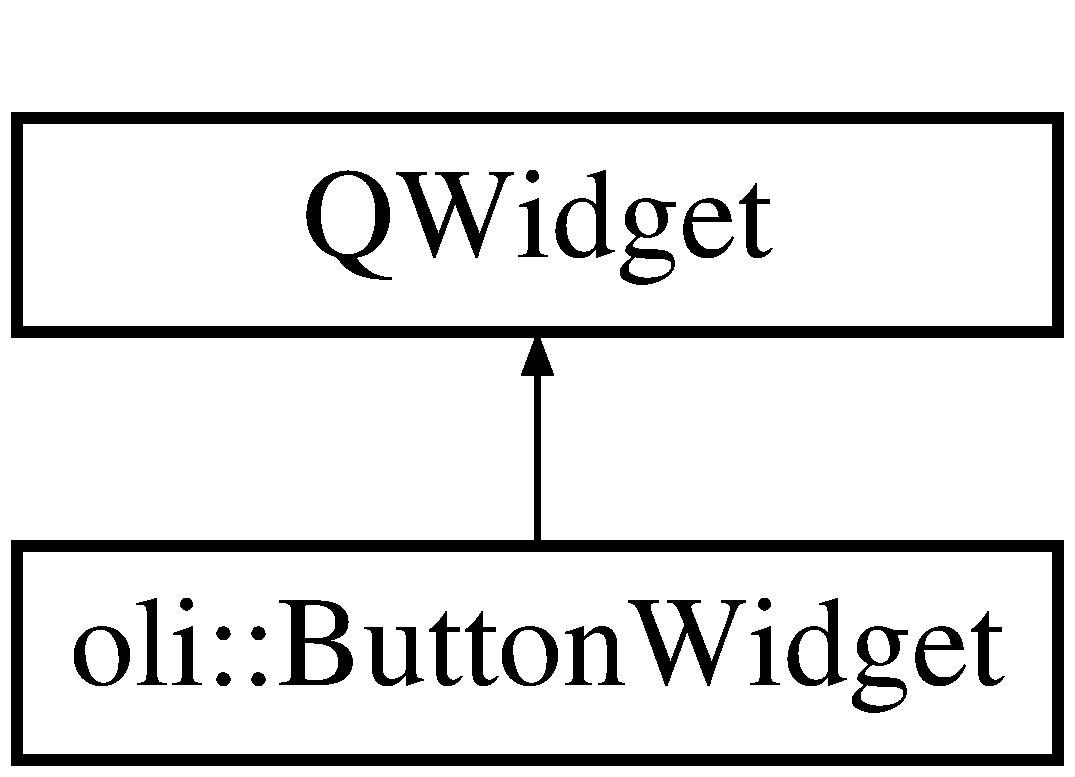
\includegraphics[height=2.000000cm]{classoli_1_1_button_widget}
\end{center}
\end{figure}
\subsection*{Signals}
\begin{DoxyCompactItemize}
\item 
void \hyperlink{classoli_1_1_button_widget_aff1ad492bde8150e865090bf98fd4c68}{clicked} (const Q\+String \&text)
\end{DoxyCompactItemize}
\subsection*{Public Member Functions}
\begin{DoxyCompactItemize}
\item 
\hyperlink{classoli_1_1_button_widget_af555496df54a4444217570f7ee49d582}{Button\+Widget} (int nb\+Col, Q\+Widget $\ast$parent=0)
\end{DoxyCompactItemize}


\subsection{Detailed Description}
The \hyperlink{classoli_1_1_button_widget}{Button\+Widget} class. 

Definition at line 17 of file buttonwidget.\+h.



\subsection{Constructor \& Destructor Documentation}
\hypertarget{classoli_1_1_button_widget_af555496df54a4444217570f7ee49d582}{}\label{classoli_1_1_button_widget_af555496df54a4444217570f7ee49d582} 
\index{oli\+::\+Button\+Widget@{oli\+::\+Button\+Widget}!Button\+Widget@{Button\+Widget}}
\index{Button\+Widget@{Button\+Widget}!oli\+::\+Button\+Widget@{oli\+::\+Button\+Widget}}
\subsubsection{\texorpdfstring{Button\+Widget()}{ButtonWidget()}}
{\footnotesize\ttfamily oli\+::\+Button\+Widget\+::\+Button\+Widget (\begin{DoxyParamCaption}\item[{int}]{nb\+Col,  }\item[{Q\+Widget $\ast$}]{parent = {\ttfamily 0} }\end{DoxyParamCaption})}



Definition at line 5 of file buttonwidget.\+cpp.


\begin{DoxyCode}
6     : QWidget(parent)
7 \{
8     signalMapper = \textcolor{keyword}{new} QSignalMapper(\textcolor{keyword}{this});
9     QGridLayout *gridLayout = \textcolor{keyword}{new} QGridLayout;
10 
11     \textcolor{keywordflow}{for} (\textcolor{keywordtype}{int} i = 1; i <= nbCol; ++i) \{
12 
13         QPushButton *button = \textcolor{keyword}{new} QPushButton(\textcolor{stringliteral}{""});
14         QColor col =\hyperlink{classoli_1_1_color_convert_a4c41280d24ad2cba4b2a46fbb03f2356}{ColorConvert::getQColor}(static\_cast<Color>(i-1));
15         QString qss = QString(\textcolor{stringliteral}{"background-color: %1"}).arg(col.name());
16         button->setStyleSheet(qss);
17         button->setFocusPolicy(Qt::NoFocus);
18         connect(button, SIGNAL(\hyperlink{classoli_1_1_button_widget_aff1ad492bde8150e865090bf98fd4c68}{clicked}()), signalMapper, SLOT(map()));
19         signalMapper->setMapping(button,i);
20         gridLayout->addWidget(button, (i-1) / 8, (i-1) % 8);
21     \}
22 
23     connect(signalMapper, SIGNAL(mapped(\textcolor{keywordtype}{int})),parent, SLOT(play(\textcolor{keywordtype}{int})));
24     setLayout(gridLayout);
25 \}
\end{DoxyCode}


\subsection{Member Function Documentation}
\hypertarget{classoli_1_1_button_widget_aff1ad492bde8150e865090bf98fd4c68}{}\label{classoli_1_1_button_widget_aff1ad492bde8150e865090bf98fd4c68} 
\index{oli\+::\+Button\+Widget@{oli\+::\+Button\+Widget}!clicked@{clicked}}
\index{clicked@{clicked}!oli\+::\+Button\+Widget@{oli\+::\+Button\+Widget}}
\subsubsection{\texorpdfstring{clicked}{clicked}}
{\footnotesize\ttfamily void oli\+::\+Button\+Widget\+::clicked (\begin{DoxyParamCaption}\item[{const Q\+String \&}]{text }\end{DoxyParamCaption})\hspace{0.3cm}{\ttfamily [signal]}}



The documentation for this class was generated from the following files\+:\begin{DoxyCompactItemize}
\item 
view/\hyperlink{buttonwidget_8h}{buttonwidget.\+h}\item 
view/\hyperlink{buttonwidget_8cpp}{buttonwidget.\+cpp}\end{DoxyCompactItemize}

\hypertarget{classoli_1_1_color_convert}{}\section{oli\+:\+:Color\+Convert Class Reference}
\label{classoli_1_1_color_convert}\index{oli\+::\+Color\+Convert@{oli\+::\+Color\+Convert}}


The \hyperlink{classoli_1_1_color_convert}{Color\+Convert} class Class used by others class to convert a color to a Q\+Color.  




{\ttfamily \#include $<$color\+Convert.\+h$>$}

\subsection*{Static Public Member Functions}
\begin{DoxyCompactItemize}
\item 
static Q\+Color \hyperlink{classoli_1_1_color_convert_a4c41280d24ad2cba4b2a46fbb03f2356}{get\+Q\+Color} (\hyperlink{namespaceoli_aac44697e43b3ab2ad32fe892ab2276eb}{Color} col)
\end{DoxyCompactItemize}


\subsection{Detailed Description}
The \hyperlink{classoli_1_1_color_convert}{Color\+Convert} class Class used by others class to convert a color to a Q\+Color. 

Definition at line 11 of file color\+Convert.\+h.



\subsection{Member Function Documentation}
\hypertarget{classoli_1_1_color_convert_a4c41280d24ad2cba4b2a46fbb03f2356}{}\label{classoli_1_1_color_convert_a4c41280d24ad2cba4b2a46fbb03f2356} 
\index{oli\+::\+Color\+Convert@{oli\+::\+Color\+Convert}!get\+Q\+Color@{get\+Q\+Color}}
\index{get\+Q\+Color@{get\+Q\+Color}!oli\+::\+Color\+Convert@{oli\+::\+Color\+Convert}}
\subsubsection{\texorpdfstring{get\+Q\+Color()}{getQColor()}}
{\footnotesize\ttfamily static Q\+Color oli\+::\+Color\+Convert\+::get\+Q\+Color (\begin{DoxyParamCaption}\item[{\hyperlink{namespaceoli_aac44697e43b3ab2ad32fe892ab2276eb}{Color}}]{col }\end{DoxyParamCaption})\hspace{0.3cm}{\ttfamily [inline]}, {\ttfamily [static]}}



Definition at line 14 of file color\+Convert.\+h.


\begin{DoxyCode}
14                                       \{
15         QColor color;
16         \textcolor{keywordflow}{switch}(col)\{
17         \textcolor{keywordflow}{case} \hyperlink{namespaceoli_aac44697e43b3ab2ad32fe892ab2276ebaa2d9547b5d3dd9f05984475f7c926da0}{Color::RED}:
18             color = Qt::red;
19             \textcolor{keywordflow}{break};
20         \textcolor{keywordflow}{case} \hyperlink{namespaceoli_aac44697e43b3ab2ad32fe892ab2276eba9de0e5dd94e861317e74964bed179fa0}{Color::GREEN}:
21             color = QColor(50,205, 50, 255);
22             \textcolor{keywordflow}{break};
23         \textcolor{keywordflow}{case} \hyperlink{namespaceoli_aac44697e43b3ab2ad32fe892ab2276eba5b6490317b6f7270bc3ab5ffd07c1f52}{Color::ORANGE}:
24             color = QColor(238, 154, 0, 255);
25             \textcolor{keywordflow}{break};
26         \textcolor{keywordflow}{case} \hyperlink{namespaceoli_aac44697e43b3ab2ad32fe892ab2276eba1b3e1ee9bff86431dea6b181365ba65f}{Color::BLUE}:
27             color = QColor(72, 118, 255, 255);
28             \textcolor{keywordflow}{break};
29         \textcolor{keywordflow}{case} \hyperlink{namespaceoli_aac44697e43b3ab2ad32fe892ab2276ebaec9c138095a352a9b7ef9ca5363b14d9}{Color::PURPLE}:
30             color =  QColor(89, 51, 204, 255);
31             \textcolor{keywordflow}{break};
32         \textcolor{keywordflow}{case} \hyperlink{namespaceoli_aac44697e43b3ab2ad32fe892ab2276eba90c86d1e3da733aaf155dcc24f2a235b}{Color::DEEPPINK}:
33             color = QColor(255, 52, 179, 255);
34             \textcolor{keywordflow}{break};
35         \textcolor{keywordflow}{case} \hyperlink{namespaceoli_aac44697e43b3ab2ad32fe892ab2276eba344dd8cd533280795b9db82ef0c92749}{Color::CYAN}:
36             color = Qt::cyan;
37             \textcolor{keywordflow}{break};
38         \textcolor{keywordflow}{case} \hyperlink{namespaceoli_aac44697e43b3ab2ad32fe892ab2276eba8a568e5f41b7e4da88fe5c4a00aad34e}{Color::YELLOW}:
39             color = Qt::yellow;
40             \textcolor{keywordflow}{break};
41         \textcolor{keywordflow}{case} \hyperlink{namespaceoli_aac44697e43b3ab2ad32fe892ab2276eba3c551f0d1a06b4f852d1832daed357bf}{Color::GREY}:
42             color = QColor(204,204,204,255);
43             \textcolor{keywordflow}{break};
44         \}
45         \textcolor{keywordflow}{return} color;
46     \}
\end{DoxyCode}


The documentation for this class was generated from the following file\+:\begin{DoxyCompactItemize}
\item 
view/\hyperlink{color_convert_8h}{color\+Convert.\+h}\end{DoxyCompactItemize}

\hypertarget{classoli_1_1_flood_exception}{}\section{oli\+:\+:Flood\+Exception Class Reference}
\label{classoli_1_1_flood_exception}\index{oli\+::\+Flood\+Exception@{oli\+::\+Flood\+Exception}}


The \hyperlink{classoli_1_1_flood_exception}{Flood\+Exception} class This is the exception class used for the game .  




{\ttfamily \#include $<$floodexception.\+h$>$}

Inheritance diagram for oli\+:\+:Flood\+Exception\+:\begin{figure}[H]
\begin{center}
\leavevmode
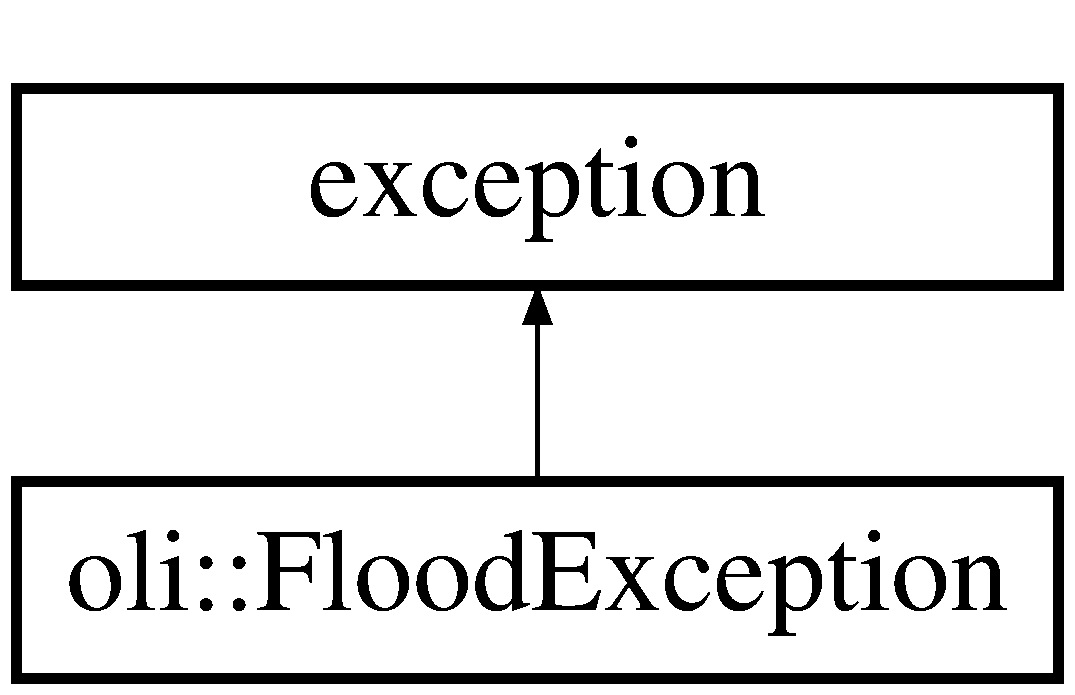
\includegraphics[height=2.000000cm]{classoli_1_1_flood_exception}
\end{center}
\end{figure}
\subsection*{Public Member Functions}
\begin{DoxyCompactItemize}
\item 
\hyperlink{classoli_1_1_flood_exception_a98d7a32c0eef6440e94cae847fa0c4ba}{Flood\+Exception} (const char $\ast$Msg)
\item 
virtual \hyperlink{classoli_1_1_flood_exception_a7c5320db13b3e5c1082ab933a6dd0bd0}{$\sim$\+Flood\+Exception} ()  throw ()
\item 
const char $\ast$ \hyperlink{classoli_1_1_flood_exception_a03204c3d2890b5de6690df657b770f72}{what} () const  throw ()
\end{DoxyCompactItemize}


\subsection{Detailed Description}
The \hyperlink{classoli_1_1_flood_exception}{Flood\+Exception} class This is the exception class used for the game . 

Definition at line 14 of file floodexception.\+h.



\subsection{Constructor \& Destructor Documentation}
\hypertarget{classoli_1_1_flood_exception_a98d7a32c0eef6440e94cae847fa0c4ba}{}\label{classoli_1_1_flood_exception_a98d7a32c0eef6440e94cae847fa0c4ba} 
\index{oli\+::\+Flood\+Exception@{oli\+::\+Flood\+Exception}!Flood\+Exception@{Flood\+Exception}}
\index{Flood\+Exception@{Flood\+Exception}!oli\+::\+Flood\+Exception@{oli\+::\+Flood\+Exception}}
\subsubsection{\texorpdfstring{Flood\+Exception()}{FloodException()}}
{\footnotesize\ttfamily oli\+::\+Flood\+Exception\+::\+Flood\+Exception (\begin{DoxyParamCaption}\item[{const char $\ast$}]{Msg }\end{DoxyParamCaption})\hspace{0.3cm}{\ttfamily [inline]}}



Definition at line 22 of file floodexception.\+h.


\begin{DoxyCode}
22                                      \{
23         std::ostringstream output;
24         output << Msg;
25         this->msg = output.str();
26     \}
\end{DoxyCode}
\hypertarget{classoli_1_1_flood_exception_a7c5320db13b3e5c1082ab933a6dd0bd0}{}\label{classoli_1_1_flood_exception_a7c5320db13b3e5c1082ab933a6dd0bd0} 
\index{oli\+::\+Flood\+Exception@{oli\+::\+Flood\+Exception}!````~Flood\+Exception@{$\sim$\+Flood\+Exception}}
\index{````~Flood\+Exception@{$\sim$\+Flood\+Exception}!oli\+::\+Flood\+Exception@{oli\+::\+Flood\+Exception}}
\subsubsection{\texorpdfstring{$\sim$\+Flood\+Exception()}{~FloodException()}}
{\footnotesize\ttfamily virtual oli\+::\+Flood\+Exception\+::$\sim$\+Flood\+Exception (\begin{DoxyParamCaption}{ }\end{DoxyParamCaption}) throw  ) \hspace{0.3cm}{\ttfamily [inline]}, {\ttfamily [virtual]}}



Definition at line 28 of file floodexception.\+h.


\begin{DoxyCode}
28 \{\}
\end{DoxyCode}


\subsection{Member Function Documentation}
\hypertarget{classoli_1_1_flood_exception_a03204c3d2890b5de6690df657b770f72}{}\label{classoli_1_1_flood_exception_a03204c3d2890b5de6690df657b770f72} 
\index{oli\+::\+Flood\+Exception@{oli\+::\+Flood\+Exception}!what@{what}}
\index{what@{what}!oli\+::\+Flood\+Exception@{oli\+::\+Flood\+Exception}}
\subsubsection{\texorpdfstring{what()}{what()}}
{\footnotesize\ttfamily const char$\ast$ oli\+::\+Flood\+Exception\+::what (\begin{DoxyParamCaption}{ }\end{DoxyParamCaption}) const throw  ) \hspace{0.3cm}{\ttfamily [inline]}}



Definition at line 30 of file floodexception.\+h.


\begin{DoxyCode}
30                                      \{
31         \textcolor{keywordflow}{return} msg.c\_str();
32     \}
\end{DoxyCode}


The documentation for this class was generated from the following file\+:\begin{DoxyCompactItemize}
\item 
model/\hyperlink{floodexception_8h}{floodexception.\+h}\end{DoxyCompactItemize}

\hypertarget{classoli_1_1_floodgame}{}\section{oli\+:\+:Floodgame Class Reference}
\label{classoli_1_1_floodgame}\index{oli\+::\+Floodgame@{oli\+::\+Floodgame}}


{\ttfamily \#include $<$floodgame.\+h$>$}

Inheritance diagram for oli\+:\+:Floodgame\+:\begin{figure}[H]
\begin{center}
\leavevmode
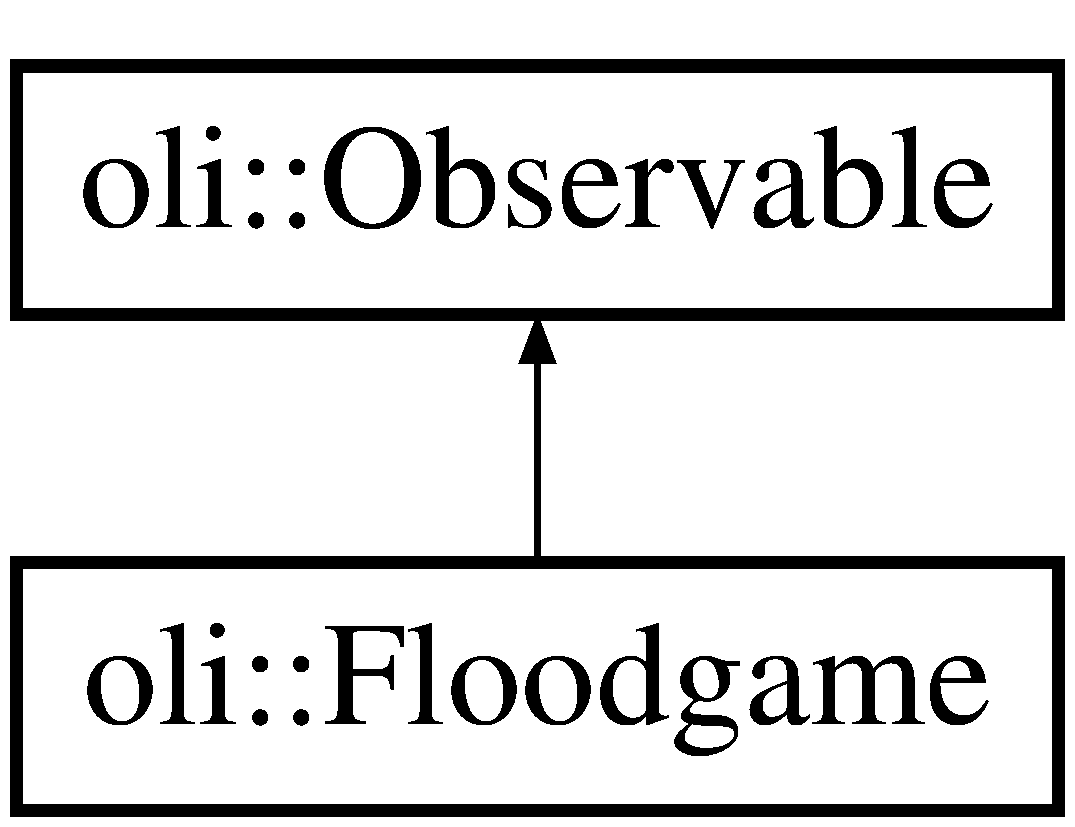
\includegraphics[height=2.000000cm]{classoli_1_1_floodgame}
\end{center}
\end{figure}
\subsection*{Public Member Functions}
\begin{DoxyCompactItemize}
\item 
\hyperlink{classoli_1_1_floodgame_ac411db6e80baa3e2a9c41d7ee71fd006}{Floodgame} (int height, int width, int nb\+Col)
\begin{DoxyCompactList}\small\item\em \hyperlink{classoli_1_1_floodgame}{Floodgame} the game\textquotesingle{}s constructor with parameters. \end{DoxyCompactList}\item 
\hyperlink{classoli_1_1_floodgame_a3e27addbd04a0eb2d27fbe05abf482f7}{$\sim$\+Floodgame} ()
\item 
\hyperlink{classoli_1_1_board}{Board} \& \hyperlink{classoli_1_1_floodgame_a4775f2321f034778d4de93a888d2283b}{get\+Board} ()
\begin{DoxyCompactList}\small\item\em get\+Board \end{DoxyCompactList}\item 
void \hyperlink{classoli_1_1_floodgame_a257b5c182fe3c40242308a6b234b75c8}{add\+Captured} (\hyperlink{classoli_1_1_position}{Position} position)
\begin{DoxyCompactList}\small\item\em add\+Captured add a \hyperlink{classoli_1_1_position}{Position} to the list of position captured \end{DoxyCompactList}\item 
int \hyperlink{classoli_1_1_floodgame_a6ffeda1d46639b093de8892b45e7bf06}{get\+Nb\+Colors} ()
\begin{DoxyCompactList}\small\item\em get\+Nb\+Colors \end{DoxyCompactList}\item 
void \hyperlink{classoli_1_1_floodgame_a2f1bf35c7c7077bccf8576324ccf60ed}{init} (int height, int width, int nb\+Col)
\begin{DoxyCompactList}\small\item\em init to initialise a new game \end{DoxyCompactList}\item 
void \hyperlink{classoli_1_1_floodgame_abf954b3e365ada491163de9ad956bd95}{flood\+Fill} (int x, int y, \hyperlink{namespaceoli_aac44697e43b3ab2ad32fe892ab2276eb}{Color} new\+Color, \hyperlink{namespaceoli_aac44697e43b3ab2ad32fe892ab2276eb}{Color} old\+Color, int cpt)
\begin{DoxyCompactList}\small\item\em flood\+Fill The algorithm to check the board for new position to capture \end{DoxyCompactList}\item 
void \hyperlink{classoli_1_1_floodgame_a371ea67d0f296c8cd3ba07e1d31cb7fe}{set\+New\+Color} (\hyperlink{namespaceoli_aac44697e43b3ab2ad32fe892ab2276eb}{Color} color)
\begin{DoxyCompactList}\small\item\em set\+New\+Color \end{DoxyCompactList}\item 
void \hyperlink{classoli_1_1_floodgame_aa6be75fd33a3181117c80529561c1f0c}{change\+Current\+Color} (\hyperlink{namespaceoli_aac44697e43b3ab2ad32fe892ab2276eb}{Color} color, int count)
\begin{DoxyCompactList}\small\item\em change\+Current\+Color \end{DoxyCompactList}\item 
bool \hyperlink{classoli_1_1_floodgame_a839915256ec11211fdbf95195c8e51cb}{get\+Is\+Game\+Over} ()
\begin{DoxyCompactList}\small\item\em get\+Is\+Game\+Over to get the gameover status \end{DoxyCompactList}\item 
void \hyperlink{classoli_1_1_floodgame_ad30fd6f491f98397de7eb46fcc96c875}{set\+Nb\+Click} ()
\begin{DoxyCompactList}\small\item\em set\+Nb\+Click to set the number of click made \end{DoxyCompactList}\item 
\hyperlink{namespaceoli_aac44697e43b3ab2ad32fe892ab2276eb}{Color} \hyperlink{classoli_1_1_floodgame_ab302cc4ae3712da0de83520cb86d9567}{get\+Last\+Color} ()
\begin{DoxyCompactList}\small\item\em get\+Last\+Color \end{DoxyCompactList}\item 
bool \hyperlink{classoli_1_1_floodgame_adfcb41900bae06b64a8d4d77164b67d5}{is\+Game\+Over} ()
\begin{DoxyCompactList}\small\item\em is\+Game\+Over \end{DoxyCompactList}\item 
bool \hyperlink{classoli_1_1_floodgame_a35b5e1c7f39c73d7d46b8c71156fbfbc}{is\+New\+Record} ()
\begin{DoxyCompactList}\small\item\em is\+New\+Record \end{DoxyCompactList}\item 
int \hyperlink{classoli_1_1_floodgame_aae08dd4e048b1521797c44a68d08f250}{get\+Nb\+Click} ()
\begin{DoxyCompactList}\small\item\em get\+Nb\+Click \end{DoxyCompactList}\item 
int \hyperlink{classoli_1_1_floodgame_af0084c4fecf2b51da6aed1f73de05e9e}{get\+Record} ()
\begin{DoxyCompactList}\small\item\em get\+Record \end{DoxyCompactList}\end{DoxyCompactItemize}


\subsection{Detailed Description}


Definition at line 17 of file floodgame.\+h.



\subsection{Constructor \& Destructor Documentation}
\hypertarget{classoli_1_1_floodgame_ac411db6e80baa3e2a9c41d7ee71fd006}{}\label{classoli_1_1_floodgame_ac411db6e80baa3e2a9c41d7ee71fd006} 
\index{oli\+::\+Floodgame@{oli\+::\+Floodgame}!Floodgame@{Floodgame}}
\index{Floodgame@{Floodgame}!oli\+::\+Floodgame@{oli\+::\+Floodgame}}
\subsubsection{\texorpdfstring{Floodgame()}{Floodgame()}}
{\footnotesize\ttfamily oli\+::\+Floodgame\+::\+Floodgame (\begin{DoxyParamCaption}\item[{int}]{height,  }\item[{int}]{width,  }\item[{int}]{nb\+Col }\end{DoxyParamCaption})}



\hyperlink{classoli_1_1_floodgame}{Floodgame} the game\textquotesingle{}s constructor with parameters. 


\begin{DoxyParams}{Parameters}
{\em height} & the board\textquotesingle{}s height \\
\hline
{\em width} & the board\textquotesingle{}s width \\
\hline
{\em nb\+Col} & the number of color possible for the squares \\
\hline
\end{DoxyParams}


Definition at line 5 of file floodgame.\+cpp.


\begin{DoxyCode}
6 \{
7     \textcolor{keywordflow}{try}
8     \{
9         \hyperlink{classoli_1_1_floodgame_a2f1bf35c7c7077bccf8576324ccf60ed}{init}(height,width,nbColors);
10     \}
11     \textcolor{keywordflow}{catch} (FloodException e)
12     \{
13         std::cerr << e.what();
14         exit(0);
15     \}
16 \}
\end{DoxyCode}
\hypertarget{classoli_1_1_floodgame_a3e27addbd04a0eb2d27fbe05abf482f7}{}\label{classoli_1_1_floodgame_a3e27addbd04a0eb2d27fbe05abf482f7} 
\index{oli\+::\+Floodgame@{oli\+::\+Floodgame}!````~Floodgame@{$\sim$\+Floodgame}}
\index{````~Floodgame@{$\sim$\+Floodgame}!oli\+::\+Floodgame@{oli\+::\+Floodgame}}
\subsubsection{\texorpdfstring{$\sim$\+Floodgame()}{~Floodgame()}}
{\footnotesize\ttfamily oli\+::\+Floodgame\+::$\sim$\+Floodgame (\begin{DoxyParamCaption}{ }\end{DoxyParamCaption})}



Definition at line 44 of file floodgame.\+cpp.


\begin{DoxyCode}
44 \{\}
\end{DoxyCode}


\subsection{Member Function Documentation}
\hypertarget{classoli_1_1_floodgame_a257b5c182fe3c40242308a6b234b75c8}{}\label{classoli_1_1_floodgame_a257b5c182fe3c40242308a6b234b75c8} 
\index{oli\+::\+Floodgame@{oli\+::\+Floodgame}!add\+Captured@{add\+Captured}}
\index{add\+Captured@{add\+Captured}!oli\+::\+Floodgame@{oli\+::\+Floodgame}}
\subsubsection{\texorpdfstring{add\+Captured()}{addCaptured()}}
{\footnotesize\ttfamily void oli\+::\+Floodgame\+::add\+Captured (\begin{DoxyParamCaption}\item[{\hyperlink{classoli_1_1_position}{Position}}]{position }\end{DoxyParamCaption})}



add\+Captured add a \hyperlink{classoli_1_1_position}{Position} to the list of position captured 


\begin{DoxyParams}{Parameters}
{\em position} & the position of the new position captured \\
\hline
\end{DoxyParams}


Definition at line 54 of file floodgame.\+cpp.


\begin{DoxyCode}
54                                             \{
55     \_listCaptured.push\_back(position);
56 \}
\end{DoxyCode}
\hypertarget{classoli_1_1_floodgame_aa6be75fd33a3181117c80529561c1f0c}{}\label{classoli_1_1_floodgame_aa6be75fd33a3181117c80529561c1f0c} 
\index{oli\+::\+Floodgame@{oli\+::\+Floodgame}!change\+Current\+Color@{change\+Current\+Color}}
\index{change\+Current\+Color@{change\+Current\+Color}!oli\+::\+Floodgame@{oli\+::\+Floodgame}}
\subsubsection{\texorpdfstring{change\+Current\+Color()}{changeCurrentColor()}}
{\footnotesize\ttfamily void oli\+::\+Floodgame\+::change\+Current\+Color (\begin{DoxyParamCaption}\item[{\hyperlink{namespaceoli_aac44697e43b3ab2ad32fe892ab2276eb}{Color}}]{color,  }\item[{int}]{count }\end{DoxyParamCaption})}



change\+Current\+Color 


\begin{DoxyParams}{Parameters}
{\em color} & the new color to set \\
\hline
{\em count} & a counter initialised \\
\hline
\end{DoxyParams}


Definition at line 58 of file floodgame.\+cpp.


\begin{DoxyCode}
58                                                      \{
59     \hyperlink{classoli_1_1_floodgame_a371ea67d0f296c8cd3ba07e1d31cb7fe}{setNewColor}(color);
60     \textcolor{keywordflow}{if} (color == \_lastColor && cpt!=0)\textcolor{keywordflow}{return};
61     \textcolor{keywordflow}{for}(Position pos: \_listCaptured)\{
62         \hyperlink{classoli_1_1_floodgame_abf954b3e365ada491163de9ad956bd95}{floodFill}(pos.getX(),pos.getY(),\_newColor,\_lastColor,cpt);
63     \}
64     \_isGameOver=\hyperlink{classoli_1_1_floodgame_adfcb41900bae06b64a8d4d77164b67d5}{isGameOver}();
65     \textcolor{keywordflow}{if}(\_isGameOver)\{
66         \_highScore = HighScore(\_board.\hyperlink{classoli_1_1_board_a228d72d2aa8a9df2f545ecef14e72a0d}{getWidth}(),\_board.\hyperlink{classoli_1_1_board_a17dce7dacfe888f52dfad0468ae51ace}{getHeight}(),\_nbClick,\_nbColors);
67         \textcolor{keywordflow}{if} (checkScores())\_newRecord=\textcolor{keyword}{true};
68     \}
69     \hyperlink{classoli_1_1_observable_ab1fe0a40f7aaa9d9acee97f8c08ec328}{Notify}();
70 \}
\end{DoxyCode}
\hypertarget{classoli_1_1_floodgame_abf954b3e365ada491163de9ad956bd95}{}\label{classoli_1_1_floodgame_abf954b3e365ada491163de9ad956bd95} 
\index{oli\+::\+Floodgame@{oli\+::\+Floodgame}!flood\+Fill@{flood\+Fill}}
\index{flood\+Fill@{flood\+Fill}!oli\+::\+Floodgame@{oli\+::\+Floodgame}}
\subsubsection{\texorpdfstring{flood\+Fill()}{floodFill()}}
{\footnotesize\ttfamily void oli\+::\+Floodgame\+::flood\+Fill (\begin{DoxyParamCaption}\item[{int}]{x,  }\item[{int}]{y,  }\item[{\hyperlink{namespaceoli_aac44697e43b3ab2ad32fe892ab2276eb}{Color}}]{new\+Color,  }\item[{\hyperlink{namespaceoli_aac44697e43b3ab2ad32fe892ab2276eb}{Color}}]{old\+Color,  }\item[{int}]{cpt }\end{DoxyParamCaption})}



flood\+Fill The algorithm to check the board for new position to capture 


\begin{DoxyParams}{Parameters}
{\em x} & the x axis position \\
\hline
{\em y} & the y axis position \\
\hline
{\em new\+Color} & the new color \\
\hline
{\em old\+Color} & the old color \\
\hline
{\em cpt} & a counter \\
\hline
\end{DoxyParams}


Definition at line 72 of file floodgame.\+cpp.


\begin{DoxyCode}
72                                                                           \{
73 
74     \textcolor{keywordflow}{if}(x<0 || y<0 || x>=\_board.\hyperlink{classoli_1_1_board_a17dce7dacfe888f52dfad0468ae51ace}{getHeight}() || y>=\_board.\hyperlink{classoli_1_1_board_a228d72d2aa8a9df2f545ecef14e72a0d}{getWidth}())\textcolor{keywordflow}{return};
75 
76     \textcolor{keywordflow}{if}(cpt==0) \_board.\hyperlink{classoli_1_1_board_a8c5091c12a29718d580db501f09592c8}{changeColorBoard}(x,y,newColor);
77     \textcolor{keywordflow}{else} \{
78         \textcolor{keywordflow}{if}(\_board.\hyperlink{classoli_1_1_board_a5c1ce624776b1169ee16d8d815e9a453}{getSquare}(x,y).\hyperlink{classoli_1_1_square_a7709b35684fb5754e53d138bb916880c}{getColor}()==newColor)\{
79             \textcolor{keywordflow}{if}(!\_board.\hyperlink{classoli_1_1_board_a5c1ce624776b1169ee16d8d815e9a453}{getSquare}(x,y).\hyperlink{classoli_1_1_square_aa8ed3521a370df288e9085222660d7ea}{getCaptured}())\{
80                 \_board.\hyperlink{classoli_1_1_board_a5c1ce624776b1169ee16d8d815e9a453}{getSquare}(x,y).\hyperlink{classoli_1_1_square_a1c2449cd8855586cd63d6bde60873ce5}{setCaptured}();
81                 \hyperlink{classoli_1_1_floodgame_a257b5c182fe3c40242308a6b234b75c8}{addCaptured}(Position(x,y));
82             \}
83         \}
84     \}
85 
86     ++cpt;
87     \textcolor{keywordflow}{if}(cpt==1)\{
88         \hyperlink{classoli_1_1_floodgame_abf954b3e365ada491163de9ad956bd95}{floodFill}(x+1, y, newColor,oldColor,cpt);
89         \hyperlink{classoli_1_1_floodgame_abf954b3e365ada491163de9ad956bd95}{floodFill}(x-1, y, newColor,oldColor,cpt);
90         \hyperlink{classoli_1_1_floodgame_abf954b3e365ada491163de9ad956bd95}{floodFill}(x, y+1, newColor,oldColor,cpt);
91         \hyperlink{classoli_1_1_floodgame_abf954b3e365ada491163de9ad956bd95}{floodFill}(x, y-1, newColor,oldColor,cpt);
92     \}
93 
94 \}
\end{DoxyCode}
\hypertarget{classoli_1_1_floodgame_a4775f2321f034778d4de93a888d2283b}{}\label{classoli_1_1_floodgame_a4775f2321f034778d4de93a888d2283b} 
\index{oli\+::\+Floodgame@{oli\+::\+Floodgame}!get\+Board@{get\+Board}}
\index{get\+Board@{get\+Board}!oli\+::\+Floodgame@{oli\+::\+Floodgame}}
\subsubsection{\texorpdfstring{get\+Board()}{getBoard()}}
{\footnotesize\ttfamily \hyperlink{classoli_1_1_board}{Board} \& oli\+::\+Floodgame\+::get\+Board (\begin{DoxyParamCaption}{ }\end{DoxyParamCaption})}



get\+Board 

\begin{DoxyReturn}{Returns}
the board 
\end{DoxyReturn}


Definition at line 46 of file floodgame.\+cpp.


\begin{DoxyCode}
46                           \{
47     \textcolor{keywordflow}{return} \_board;
48 \}
\end{DoxyCode}
\hypertarget{classoli_1_1_floodgame_a839915256ec11211fdbf95195c8e51cb}{}\label{classoli_1_1_floodgame_a839915256ec11211fdbf95195c8e51cb} 
\index{oli\+::\+Floodgame@{oli\+::\+Floodgame}!get\+Is\+Game\+Over@{get\+Is\+Game\+Over}}
\index{get\+Is\+Game\+Over@{get\+Is\+Game\+Over}!oli\+::\+Floodgame@{oli\+::\+Floodgame}}
\subsubsection{\texorpdfstring{get\+Is\+Game\+Over()}{getIsGameOver()}}
{\footnotesize\ttfamily bool oli\+::\+Floodgame\+::get\+Is\+Game\+Over (\begin{DoxyParamCaption}{ }\end{DoxyParamCaption})}



get\+Is\+Game\+Over to get the gameover status 

\begin{DoxyReturn}{Returns}
if the game is over or not 
\end{DoxyReturn}


Definition at line 105 of file floodgame.\+cpp.


\begin{DoxyCode}
105                              \{
106     \textcolor{keywordflow}{return} \_isGameOver;
107 \}
\end{DoxyCode}
\hypertarget{classoli_1_1_floodgame_ab302cc4ae3712da0de83520cb86d9567}{}\label{classoli_1_1_floodgame_ab302cc4ae3712da0de83520cb86d9567} 
\index{oli\+::\+Floodgame@{oli\+::\+Floodgame}!get\+Last\+Color@{get\+Last\+Color}}
\index{get\+Last\+Color@{get\+Last\+Color}!oli\+::\+Floodgame@{oli\+::\+Floodgame}}
\subsubsection{\texorpdfstring{get\+Last\+Color()}{getLastColor()}}
{\footnotesize\ttfamily \hyperlink{namespaceoli_aac44697e43b3ab2ad32fe892ab2276eb}{Color} oli\+::\+Floodgame\+::get\+Last\+Color (\begin{DoxyParamCaption}{ }\end{DoxyParamCaption})}



get\+Last\+Color 

\begin{DoxyReturn}{Returns}
the last color choosed 
\end{DoxyReturn}


Definition at line 109 of file floodgame.\+cpp.


\begin{DoxyCode}
109                              \{
110     \textcolor{keywordflow}{return} \_newColor;
111 \}
\end{DoxyCode}
\hypertarget{classoli_1_1_floodgame_aae08dd4e048b1521797c44a68d08f250}{}\label{classoli_1_1_floodgame_aae08dd4e048b1521797c44a68d08f250} 
\index{oli\+::\+Floodgame@{oli\+::\+Floodgame}!get\+Nb\+Click@{get\+Nb\+Click}}
\index{get\+Nb\+Click@{get\+Nb\+Click}!oli\+::\+Floodgame@{oli\+::\+Floodgame}}
\subsubsection{\texorpdfstring{get\+Nb\+Click()}{getNbClick()}}
{\footnotesize\ttfamily int oli\+::\+Floodgame\+::get\+Nb\+Click (\begin{DoxyParamCaption}{ }\end{DoxyParamCaption})}



get\+Nb\+Click 

\begin{DoxyReturn}{Returns}
the number of click 
\end{DoxyReturn}


Definition at line 121 of file floodgame.\+cpp.


\begin{DoxyCode}
121                          \{
122     \textcolor{keywordflow}{return} \_nbClick;
123 \}
\end{DoxyCode}
\hypertarget{classoli_1_1_floodgame_a6ffeda1d46639b093de8892b45e7bf06}{}\label{classoli_1_1_floodgame_a6ffeda1d46639b093de8892b45e7bf06} 
\index{oli\+::\+Floodgame@{oli\+::\+Floodgame}!get\+Nb\+Colors@{get\+Nb\+Colors}}
\index{get\+Nb\+Colors@{get\+Nb\+Colors}!oli\+::\+Floodgame@{oli\+::\+Floodgame}}
\subsubsection{\texorpdfstring{get\+Nb\+Colors()}{getNbColors()}}
{\footnotesize\ttfamily int oli\+::\+Floodgame\+::get\+Nb\+Colors (\begin{DoxyParamCaption}{ }\end{DoxyParamCaption})}



get\+Nb\+Colors 

\begin{DoxyReturn}{Returns}
the number of color possible for a square 
\end{DoxyReturn}


Definition at line 50 of file floodgame.\+cpp.


\begin{DoxyCode}
50                           \{
51     \textcolor{keywordflow}{return} \_nbColors;
52 \}
\end{DoxyCode}
\hypertarget{classoli_1_1_floodgame_af0084c4fecf2b51da6aed1f73de05e9e}{}\label{classoli_1_1_floodgame_af0084c4fecf2b51da6aed1f73de05e9e} 
\index{oli\+::\+Floodgame@{oli\+::\+Floodgame}!get\+Record@{get\+Record}}
\index{get\+Record@{get\+Record}!oli\+::\+Floodgame@{oli\+::\+Floodgame}}
\subsubsection{\texorpdfstring{get\+Record()}{getRecord()}}
{\footnotesize\ttfamily int oli\+::\+Floodgame\+::get\+Record (\begin{DoxyParamCaption}{ }\end{DoxyParamCaption})}



get\+Record 

\begin{DoxyReturn}{Returns}
the record 
\end{DoxyReturn}


Definition at line 165 of file floodgame.\+cpp.


\begin{DoxyCode}
165                         \{
166     QJsonObject gameObject;
167     gameObject =loadSavedScores();
168     QString \textcolor{keywordtype}{id} =\_highScore.\hyperlink{classoli_1_1_high_score_ae0c11fdb5f35199aa785d6e66bfe8d03}{getId}();
169 
170     \textcolor{keywordflow}{if}(gameObject.contains(\textcolor{keywordtype}{id}))\{
171         \textcolor{keywordflow}{return} gameObject.value(\textcolor{keywordtype}{id}).toInt();
172     \}
173     \textcolor{keywordflow}{else}\{
174         \textcolor{keywordflow}{return} 0;
175     \}
176 
177 \}
\end{DoxyCode}
\hypertarget{classoli_1_1_floodgame_a2f1bf35c7c7077bccf8576324ccf60ed}{}\label{classoli_1_1_floodgame_a2f1bf35c7c7077bccf8576324ccf60ed} 
\index{oli\+::\+Floodgame@{oli\+::\+Floodgame}!init@{init}}
\index{init@{init}!oli\+::\+Floodgame@{oli\+::\+Floodgame}}
\subsubsection{\texorpdfstring{init()}{init()}}
{\footnotesize\ttfamily void oli\+::\+Floodgame\+::init (\begin{DoxyParamCaption}\item[{int}]{height,  }\item[{int}]{width,  }\item[{int}]{nb\+Col }\end{DoxyParamCaption})}



init to initialise a new game 


\begin{DoxyParams}{Parameters}
{\em height} & the board\textquotesingle{}s height \\
\hline
{\em width} & the board\textquotesingle{}s width \\
\hline
{\em nb\+Col} & the number of different color possible for the squares \\
\hline
\end{DoxyParams}


Definition at line 18 of file floodgame.\+cpp.


\begin{DoxyCode}
18                                                   \{
19     \_nbClick = 0;
20     \_isGameOver = \textcolor{keyword}{false};
21     \_nbColors = nbCol;
22     \_started = \textcolor{keyword}{true};
23     \_isGameOver = \textcolor{keyword}{false};
24     \textcolor{keywordflow}{try}
25     \{
26         \_board = Board(height,width,\_nbColors);
27     \}
28     \textcolor{keywordflow}{catch} (FloodException e)
29     \{
30         std::cerr << e.what();
31         exit(0);
32     \}
33 
34     \_listCaptured.clear();
35     \_listCaptured.push\_back(Position(0,0));
36     \_lastColor = \_board.\hyperlink{classoli_1_1_board_a5c1ce624776b1169ee16d8d815e9a453}{getSquare}(0,0).\hyperlink{classoli_1_1_square_a7709b35684fb5754e53d138bb916880c}{getColor}();
37     \_newColor = \_board.\hyperlink{classoli_1_1_board_a5c1ce624776b1169ee16d8d815e9a453}{getSquare}(0,0).\hyperlink{classoli_1_1_square_a7709b35684fb5754e53d138bb916880c}{getColor}();
38     this->\hyperlink{classoli_1_1_floodgame_aa6be75fd33a3181117c80529561c1f0c}{changeCurrentColor}(\_lastColor,0);
39     \_highScore = HighScore(\_board.\hyperlink{classoli_1_1_board_a228d72d2aa8a9df2f545ecef14e72a0d}{getWidth}(),\_board.\hyperlink{classoli_1_1_board_a17dce7dacfe888f52dfad0468ae51ace}{getHeight}(),\_nbColors);
40     \_newRecord = \textcolor{keyword}{false};
41 
42 \}
\end{DoxyCode}
\hypertarget{classoli_1_1_floodgame_adfcb41900bae06b64a8d4d77164b67d5}{}\label{classoli_1_1_floodgame_adfcb41900bae06b64a8d4d77164b67d5} 
\index{oli\+::\+Floodgame@{oli\+::\+Floodgame}!is\+Game\+Over@{is\+Game\+Over}}
\index{is\+Game\+Over@{is\+Game\+Over}!oli\+::\+Floodgame@{oli\+::\+Floodgame}}
\subsubsection{\texorpdfstring{is\+Game\+Over()}{isGameOver()}}
{\footnotesize\ttfamily bool oli\+::\+Floodgame\+::is\+Game\+Over (\begin{DoxyParamCaption}{ }\end{DoxyParamCaption})}



is\+Game\+Over 

\begin{DoxyReturn}{Returns}
if the game is over or not 
\end{DoxyReturn}


Definition at line 101 of file floodgame.\+cpp.


\begin{DoxyCode}
101                           \{
102     \textcolor{keywordflow}{return} \textcolor{keyword}{static\_cast<}\textcolor{keywordtype}{int}\textcolor{keyword}{>}(\_listCaptured.size())==\_board.\hyperlink{classoli_1_1_board_a228d72d2aa8a9df2f545ecef14e72a0d}{getWidth}()*\_board.
      \hyperlink{classoli_1_1_board_a17dce7dacfe888f52dfad0468ae51ace}{getHeight}();
103 \}
\end{DoxyCode}
\hypertarget{classoli_1_1_floodgame_a35b5e1c7f39c73d7d46b8c71156fbfbc}{}\label{classoli_1_1_floodgame_a35b5e1c7f39c73d7d46b8c71156fbfbc} 
\index{oli\+::\+Floodgame@{oli\+::\+Floodgame}!is\+New\+Record@{is\+New\+Record}}
\index{is\+New\+Record@{is\+New\+Record}!oli\+::\+Floodgame@{oli\+::\+Floodgame}}
\subsubsection{\texorpdfstring{is\+New\+Record()}{isNewRecord()}}
{\footnotesize\ttfamily bool oli\+::\+Floodgame\+::is\+New\+Record (\begin{DoxyParamCaption}{ }\end{DoxyParamCaption})}



is\+New\+Record 

\begin{DoxyReturn}{Returns}
if the actual score is a new record or not 
\end{DoxyReturn}


Definition at line 117 of file floodgame.\+cpp.


\begin{DoxyCode}
117                            \{
118     \textcolor{keywordflow}{return} \_newRecord;
119 \}
\end{DoxyCode}
\hypertarget{classoli_1_1_floodgame_ad30fd6f491f98397de7eb46fcc96c875}{}\label{classoli_1_1_floodgame_ad30fd6f491f98397de7eb46fcc96c875} 
\index{oli\+::\+Floodgame@{oli\+::\+Floodgame}!set\+Nb\+Click@{set\+Nb\+Click}}
\index{set\+Nb\+Click@{set\+Nb\+Click}!oli\+::\+Floodgame@{oli\+::\+Floodgame}}
\subsubsection{\texorpdfstring{set\+Nb\+Click()}{setNbClick()}}
{\footnotesize\ttfamily void oli\+::\+Floodgame\+::set\+Nb\+Click (\begin{DoxyParamCaption}{ }\end{DoxyParamCaption})}



set\+Nb\+Click to set the number of click made 



Definition at line 113 of file floodgame.\+cpp.


\begin{DoxyCode}
113                           \{
114     ++\_nbClick;
115 \}
\end{DoxyCode}
\hypertarget{classoli_1_1_floodgame_a371ea67d0f296c8cd3ba07e1d31cb7fe}{}\label{classoli_1_1_floodgame_a371ea67d0f296c8cd3ba07e1d31cb7fe} 
\index{oli\+::\+Floodgame@{oli\+::\+Floodgame}!set\+New\+Color@{set\+New\+Color}}
\index{set\+New\+Color@{set\+New\+Color}!oli\+::\+Floodgame@{oli\+::\+Floodgame}}
\subsubsection{\texorpdfstring{set\+New\+Color()}{setNewColor()}}
{\footnotesize\ttfamily void oli\+::\+Floodgame\+::set\+New\+Color (\begin{DoxyParamCaption}\item[{\hyperlink{namespaceoli_aac44697e43b3ab2ad32fe892ab2276eb}{Color}}]{color }\end{DoxyParamCaption})}



set\+New\+Color 


\begin{DoxyParams}{Parameters}
{\em color} & the new color to set \\
\hline
\end{DoxyParams}


Definition at line 96 of file floodgame.\+cpp.


\begin{DoxyCode}
96                                       \{
97     \_lastColor = \_newColor;
98     \_newColor = color;
99 \}
\end{DoxyCode}


The documentation for this class was generated from the following files\+:\begin{DoxyCompactItemize}
\item 
model/\hyperlink{floodgame_8h}{floodgame.\+h}\item 
model/\hyperlink{floodgame_8cpp}{floodgame.\+cpp}\end{DoxyCompactItemize}

\hypertarget{classoli_1_1_high_score}{}\section{oli\+:\+:High\+Score Class Reference}
\label{classoli_1_1_high_score}\index{oli\+::\+High\+Score@{oli\+::\+High\+Score}}


The \hyperlink{classoli_1_1_high_score}{High\+Score} class Used to compare old results and the new score according to the weight, the height and the number of colors function.  




{\ttfamily \#include $<$High\+Score.\+h$>$}

\subsection*{Public Member Functions}
\begin{DoxyCompactItemize}
\item 
\hyperlink{classoli_1_1_high_score_a0d912d7674165be2873897b1d62ccccf}{High\+Score} ()
\begin{DoxyCompactList}\small\item\em \hyperlink{classoli_1_1_high_score}{High\+Score}. \end{DoxyCompactList}\item 
\hyperlink{classoli_1_1_high_score_ac59979c25b9bb0d937f883dcb66a6db5}{High\+Score} (int, int, int, int)
\begin{DoxyCompactList}\small\item\em \hyperlink{classoli_1_1_high_score}{High\+Score} highscore\textquotesingle{}s constructor with parameters. \end{DoxyCompactList}\item 
\hyperlink{classoli_1_1_high_score_aa7566dd6d1287aa5c9a248248bf61b59}{High\+Score} (int, int, int)
\begin{DoxyCompactList}\small\item\em \hyperlink{classoli_1_1_high_score}{High\+Score} highscore\textquotesingle{}s constructor with parameters. \end{DoxyCompactList}\item 
void \hyperlink{classoli_1_1_high_score_a161063aa9576b92bf4d1f64af7a7850c}{set\+Width} (int)
\begin{DoxyCompactList}\small\item\em set\+Width to set the width \end{DoxyCompactList}\item 
void \hyperlink{classoli_1_1_high_score_aa3e83b28bf2f086cc19f2049d508fe03}{set\+Height} (int)
\begin{DoxyCompactList}\small\item\em set\+Height to set the height \end{DoxyCompactList}\item 
void \hyperlink{classoli_1_1_high_score_a2a8626c74ae1c37f49bd4334600f493c}{set\+Best} (int)
\begin{DoxyCompactList}\small\item\em set\+Best to set the best score \end{DoxyCompactList}\item 
void \hyperlink{classoli_1_1_high_score_a1f4db3a9679c923b21530a91d17d40fa}{set\+Nb\+Colors} (int)
\begin{DoxyCompactList}\small\item\em set\+Nb\+Colors \end{DoxyCompactList}\item 
Q\+String \hyperlink{classoli_1_1_high_score_ae0c11fdb5f35199aa785d6e66bfe8d03}{get\+Id} () const
\begin{DoxyCompactList}\small\item\em get\+Id \end{DoxyCompactList}\item 
int \hyperlink{classoli_1_1_high_score_a22d70136ee71bd13be26e30a423e0e7f}{get\+Best} () const
\begin{DoxyCompactList}\small\item\em get\+Best \end{DoxyCompactList}\item 
void \hyperlink{classoli_1_1_high_score_a644fb39e171f4176159168fed4b31753}{write} (Q\+Json\+Object \&json) const
\begin{DoxyCompactList}\small\item\em write write into a Json object the id of a highscore and the score associated \end{DoxyCompactList}\end{DoxyCompactItemize}


\subsection{Detailed Description}
The \hyperlink{classoli_1_1_high_score}{High\+Score} class Used to compare old results and the new score according to the weight, the height and the number of colors function. 

Definition at line 15 of file High\+Score.\+h.



\subsection{Constructor \& Destructor Documentation}
\hypertarget{classoli_1_1_high_score_a0d912d7674165be2873897b1d62ccccf}{}\label{classoli_1_1_high_score_a0d912d7674165be2873897b1d62ccccf} 
\index{oli\+::\+High\+Score@{oli\+::\+High\+Score}!High\+Score@{High\+Score}}
\index{High\+Score@{High\+Score}!oli\+::\+High\+Score@{oli\+::\+High\+Score}}
\subsubsection{\texorpdfstring{High\+Score()}{HighScore()}\hspace{0.1cm}{\footnotesize\ttfamily [1/3]}}
{\footnotesize\ttfamily oli\+::\+High\+Score\+::\+High\+Score (\begin{DoxyParamCaption}{ }\end{DoxyParamCaption})}



\hyperlink{classoli_1_1_high_score}{High\+Score}. 



Definition at line 5 of file High\+Score.\+cpp.


\begin{DoxyCode}
5 \{\}
\end{DoxyCode}
\hypertarget{classoli_1_1_high_score_ac59979c25b9bb0d937f883dcb66a6db5}{}\label{classoli_1_1_high_score_ac59979c25b9bb0d937f883dcb66a6db5} 
\index{oli\+::\+High\+Score@{oli\+::\+High\+Score}!High\+Score@{High\+Score}}
\index{High\+Score@{High\+Score}!oli\+::\+High\+Score@{oli\+::\+High\+Score}}
\subsubsection{\texorpdfstring{High\+Score()}{HighScore()}\hspace{0.1cm}{\footnotesize\ttfamily [2/3]}}
{\footnotesize\ttfamily oli\+::\+High\+Score\+::\+High\+Score (\begin{DoxyParamCaption}\item[{int}]{width,  }\item[{int}]{height,  }\item[{int}]{best,  }\item[{int}]{nb\+Colors }\end{DoxyParamCaption})}



\hyperlink{classoli_1_1_high_score}{High\+Score} highscore\textquotesingle{}s constructor with parameters. 



Definition at line 11 of file High\+Score.\+cpp.


\begin{DoxyCode}
11                                                               \{
12     \_width = width;
13     \_height = height;
14     \_nbColors = nbColors;
15     \_best = best; 
16 \}
\end{DoxyCode}
\hypertarget{classoli_1_1_high_score_aa7566dd6d1287aa5c9a248248bf61b59}{}\label{classoli_1_1_high_score_aa7566dd6d1287aa5c9a248248bf61b59} 
\index{oli\+::\+High\+Score@{oli\+::\+High\+Score}!High\+Score@{High\+Score}}
\index{High\+Score@{High\+Score}!oli\+::\+High\+Score@{oli\+::\+High\+Score}}
\subsubsection{\texorpdfstring{High\+Score()}{HighScore()}\hspace{0.1cm}{\footnotesize\ttfamily [3/3]}}
{\footnotesize\ttfamily oli\+::\+High\+Score\+::\+High\+Score (\begin{DoxyParamCaption}\item[{int}]{width,  }\item[{int}]{height,  }\item[{int}]{nb\+Colors }\end{DoxyParamCaption})}



\hyperlink{classoli_1_1_high_score}{High\+Score} highscore\textquotesingle{}s constructor with parameters. 



Definition at line 6 of file High\+Score.\+cpp.


\begin{DoxyCode}
6                                                      \{
7     \_width = width;
8     \_height = height;
9     \_nbColors = nbColors;
10 \}
\end{DoxyCode}


\subsection{Member Function Documentation}
\hypertarget{classoli_1_1_high_score_a22d70136ee71bd13be26e30a423e0e7f}{}\label{classoli_1_1_high_score_a22d70136ee71bd13be26e30a423e0e7f} 
\index{oli\+::\+High\+Score@{oli\+::\+High\+Score}!get\+Best@{get\+Best}}
\index{get\+Best@{get\+Best}!oli\+::\+High\+Score@{oli\+::\+High\+Score}}
\subsubsection{\texorpdfstring{get\+Best()}{getBest()}}
{\footnotesize\ttfamily int oli\+::\+High\+Score\+::get\+Best (\begin{DoxyParamCaption}{ }\end{DoxyParamCaption}) const}



get\+Best 

\begin{DoxyReturn}{Returns}
the best score 
\end{DoxyReturn}


Definition at line 48 of file High\+Score.\+cpp.


\begin{DoxyCode}
48                             \{
49     \textcolor{keywordflow}{return} \_best;
50 \}
\end{DoxyCode}
\hypertarget{classoli_1_1_high_score_ae0c11fdb5f35199aa785d6e66bfe8d03}{}\label{classoli_1_1_high_score_ae0c11fdb5f35199aa785d6e66bfe8d03} 
\index{oli\+::\+High\+Score@{oli\+::\+High\+Score}!get\+Id@{get\+Id}}
\index{get\+Id@{get\+Id}!oli\+::\+High\+Score@{oli\+::\+High\+Score}}
\subsubsection{\texorpdfstring{get\+Id()}{getId()}}
{\footnotesize\ttfamily Q\+String oli\+::\+High\+Score\+::get\+Id (\begin{DoxyParamCaption}{ }\end{DoxyParamCaption}) const}



get\+Id 

\begin{DoxyReturn}{Returns}
the id which defines the game record according to the weight, the height and the number of colors 
\end{DoxyReturn}


Definition at line 44 of file High\+Score.\+cpp.


\begin{DoxyCode}
44                               \{
45    \textcolor{keywordflow}{return} format(\_width) + format(\_height) + format(\_nbColors);
46 \}
\end{DoxyCode}
\hypertarget{classoli_1_1_high_score_a2a8626c74ae1c37f49bd4334600f493c}{}\label{classoli_1_1_high_score_a2a8626c74ae1c37f49bd4334600f493c} 
\index{oli\+::\+High\+Score@{oli\+::\+High\+Score}!set\+Best@{set\+Best}}
\index{set\+Best@{set\+Best}!oli\+::\+High\+Score@{oli\+::\+High\+Score}}
\subsubsection{\texorpdfstring{set\+Best()}{setBest()}}
{\footnotesize\ttfamily void oli\+::\+High\+Score\+::set\+Best (\begin{DoxyParamCaption}\item[{int}]{best }\end{DoxyParamCaption})}



set\+Best to set the best score 



Definition at line 23 of file High\+Score.\+cpp.


\begin{DoxyCode}
23                                \{
24     \_best = best;
25 \}
\end{DoxyCode}
\hypertarget{classoli_1_1_high_score_aa3e83b28bf2f086cc19f2049d508fe03}{}\label{classoli_1_1_high_score_aa3e83b28bf2f086cc19f2049d508fe03} 
\index{oli\+::\+High\+Score@{oli\+::\+High\+Score}!set\+Height@{set\+Height}}
\index{set\+Height@{set\+Height}!oli\+::\+High\+Score@{oli\+::\+High\+Score}}
\subsubsection{\texorpdfstring{set\+Height()}{setHeight()}}
{\footnotesize\ttfamily void oli\+::\+High\+Score\+::set\+Height (\begin{DoxyParamCaption}\item[{int}]{height }\end{DoxyParamCaption})}



set\+Height to set the height 



Definition at line 20 of file High\+Score.\+cpp.


\begin{DoxyCode}
20                                    \{
21     \_height = height;
22 \}
\end{DoxyCode}
\hypertarget{classoli_1_1_high_score_a1f4db3a9679c923b21530a91d17d40fa}{}\label{classoli_1_1_high_score_a1f4db3a9679c923b21530a91d17d40fa} 
\index{oli\+::\+High\+Score@{oli\+::\+High\+Score}!set\+Nb\+Colors@{set\+Nb\+Colors}}
\index{set\+Nb\+Colors@{set\+Nb\+Colors}!oli\+::\+High\+Score@{oli\+::\+High\+Score}}
\subsubsection{\texorpdfstring{set\+Nb\+Colors()}{setNbColors()}}
{\footnotesize\ttfamily void oli\+::\+High\+Score\+::set\+Nb\+Colors (\begin{DoxyParamCaption}\item[{int}]{nb\+Colors }\end{DoxyParamCaption})}



set\+Nb\+Colors 



Definition at line 26 of file High\+Score.\+cpp.


\begin{DoxyCode}
26                                        \{
27     \_nbColors = nbColors;
28 \}
\end{DoxyCode}
\hypertarget{classoli_1_1_high_score_a161063aa9576b92bf4d1f64af7a7850c}{}\label{classoli_1_1_high_score_a161063aa9576b92bf4d1f64af7a7850c} 
\index{oli\+::\+High\+Score@{oli\+::\+High\+Score}!set\+Width@{set\+Width}}
\index{set\+Width@{set\+Width}!oli\+::\+High\+Score@{oli\+::\+High\+Score}}
\subsubsection{\texorpdfstring{set\+Width()}{setWidth()}}
{\footnotesize\ttfamily void oli\+::\+High\+Score\+::set\+Width (\begin{DoxyParamCaption}\item[{int}]{width }\end{DoxyParamCaption})}



set\+Width to set the width 



Definition at line 17 of file High\+Score.\+cpp.


\begin{DoxyCode}
17                                  \{
18     \_width = width;
19 \}
\end{DoxyCode}
\hypertarget{classoli_1_1_high_score_a644fb39e171f4176159168fed4b31753}{}\label{classoli_1_1_high_score_a644fb39e171f4176159168fed4b31753} 
\index{oli\+::\+High\+Score@{oli\+::\+High\+Score}!write@{write}}
\index{write@{write}!oli\+::\+High\+Score@{oli\+::\+High\+Score}}
\subsubsection{\texorpdfstring{write()}{write()}}
{\footnotesize\ttfamily void oli\+::\+High\+Score\+::write (\begin{DoxyParamCaption}\item[{Q\+Json\+Object \&}]{json }\end{DoxyParamCaption}) const}



write write into a Json object the id of a highscore and the score associated 


\begin{DoxyParams}{Parameters}
{\em json} & \\
\hline
\end{DoxyParams}


Definition at line 30 of file High\+Score.\+cpp.


\begin{DoxyCode}
30                                             \{
31     QString id;
32     \textcolor{keywordtype}{id} = format(\_width) + format(\_height) + format(\_nbColors);
33     json[id] = \_best;
34 \}
\end{DoxyCode}


The documentation for this class was generated from the following files\+:\begin{DoxyCompactItemize}
\item 
model/\hyperlink{_high_score_8h}{High\+Score.\+h}\item 
model/\hyperlink{_high_score_8cpp}{High\+Score.\+cpp}\end{DoxyCompactItemize}

\hypertarget{class_intro}{}\section{Intro Class Reference}
\label{class_intro}\index{Intro@{Intro}}


The \hyperlink{class_intro}{Intro} class The class launched during a few seconds at the begining of the program launch.  




{\ttfamily \#include $<$intro.\+h$>$}

Inheritance diagram for Intro\+:\begin{figure}[H]
\begin{center}
\leavevmode
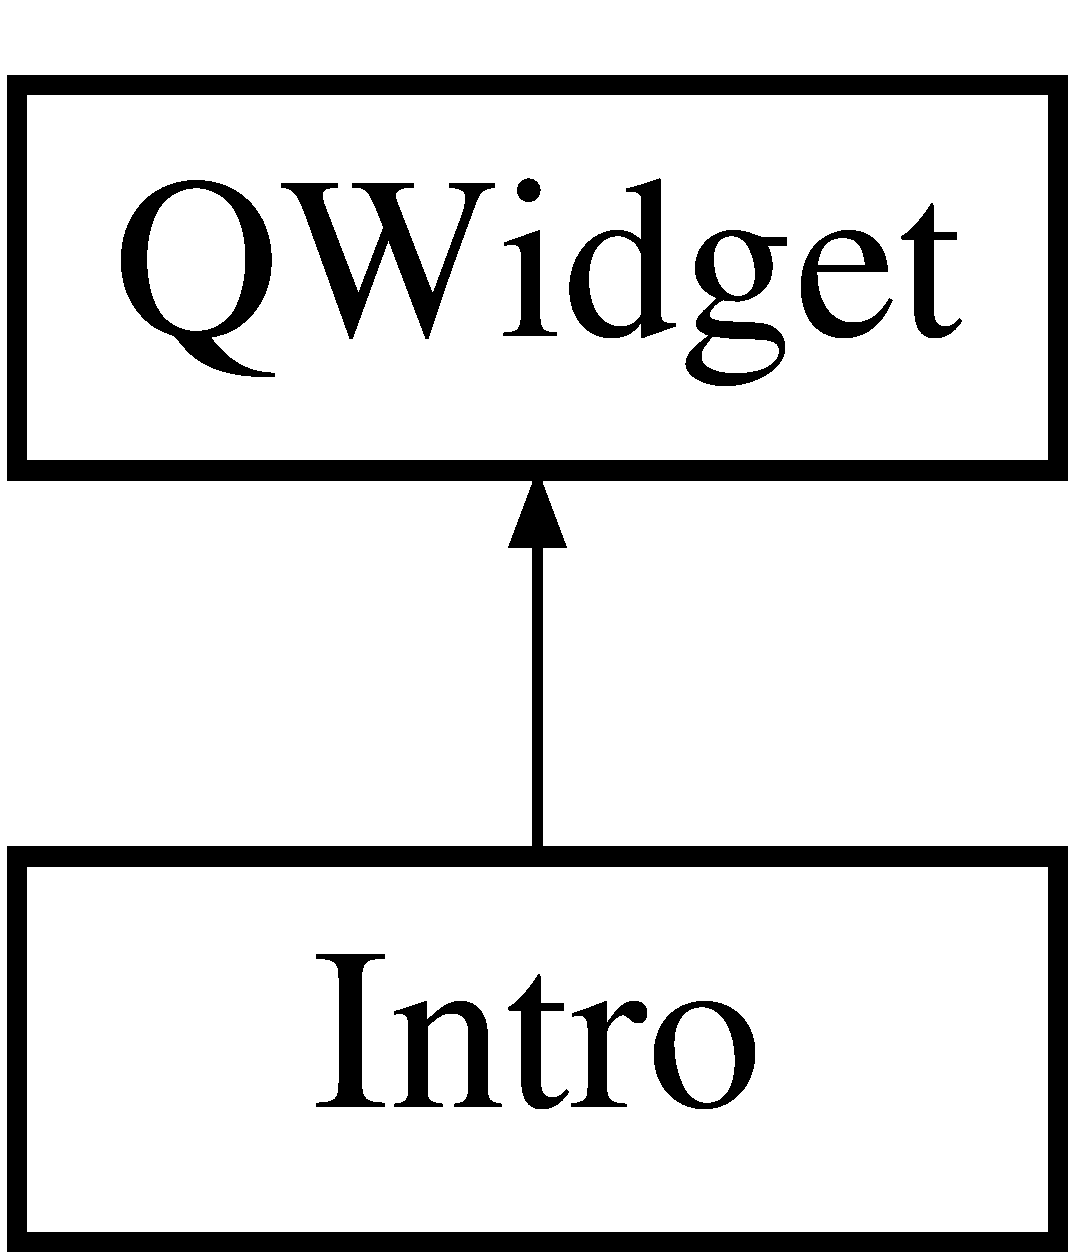
\includegraphics[height=2.000000cm]{class_intro}
\end{center}
\end{figure}
\subsection*{Public Member Functions}
\begin{DoxyCompactItemize}
\item 
\hyperlink{class_intro_a82415c2693757f51e4e93ccc8abd720e}{Intro} (Q\+Widget $\ast$parent=0)
\item 
\hyperlink{class_intro_a024067dadaf97daca3bfeb0f22e9c183}{$\sim$\+Intro} ()
\end{DoxyCompactItemize}


\subsection{Detailed Description}
The \hyperlink{class_intro}{Intro} class The class launched during a few seconds at the begining of the program launch. 

Definition at line 17 of file intro.\+h.



\subsection{Constructor \& Destructor Documentation}
\hypertarget{class_intro_a82415c2693757f51e4e93ccc8abd720e}{}\label{class_intro_a82415c2693757f51e4e93ccc8abd720e} 
\index{Intro@{Intro}!Intro@{Intro}}
\index{Intro@{Intro}!Intro@{Intro}}
\subsubsection{\texorpdfstring{Intro()}{Intro()}}
{\footnotesize\ttfamily Intro\+::\+Intro (\begin{DoxyParamCaption}\item[{Q\+Widget $\ast$}]{parent = {\ttfamily 0} }\end{DoxyParamCaption})\hspace{0.3cm}{\ttfamily [explicit]}}



Definition at line 3 of file intro.\+cpp.


\begin{DoxyCode}
3                             :
4     QWidget(parent)
5 \{
6     QPixmap bkgnd(\textcolor{stringliteral}{":/images/intro.jpg"});
7     QPalette palette;
8     palette.setBrush(QPalette::Background, bkgnd);
9     parent->setPalette(palette);
10     this->setFixedSize(720,660);
11 \}
\end{DoxyCode}
\hypertarget{class_intro_a024067dadaf97daca3bfeb0f22e9c183}{}\label{class_intro_a024067dadaf97daca3bfeb0f22e9c183} 
\index{Intro@{Intro}!````~Intro@{$\sim$\+Intro}}
\index{````~Intro@{$\sim$\+Intro}!Intro@{Intro}}
\subsubsection{\texorpdfstring{$\sim$\+Intro()}{~Intro()}}
{\footnotesize\ttfamily Intro\+::$\sim$\+Intro (\begin{DoxyParamCaption}{ }\end{DoxyParamCaption})}



Definition at line 13 of file intro.\+cpp.


\begin{DoxyCode}
13 \{\}
\end{DoxyCode}


The documentation for this class was generated from the following files\+:\begin{DoxyCompactItemize}
\item 
view/\hyperlink{intro_8h}{intro.\+h}\item 
view/\hyperlink{intro_8cpp}{intro.\+cpp}\end{DoxyCompactItemize}

\hypertarget{class_main_window}{}\section{Main\+Window Class Reference}
\label{class_main_window}\index{Main\+Window@{Main\+Window}}


The \hyperlink{class_main_window}{Main\+Window} class The application\textquotesingle{}s controller This class manage the different view of the application and the has the game object.  




{\ttfamily \#include $<$mainwindow.\+h$>$}

Inheritance diagram for Main\+Window\+:\begin{figure}[H]
\begin{center}
\leavevmode
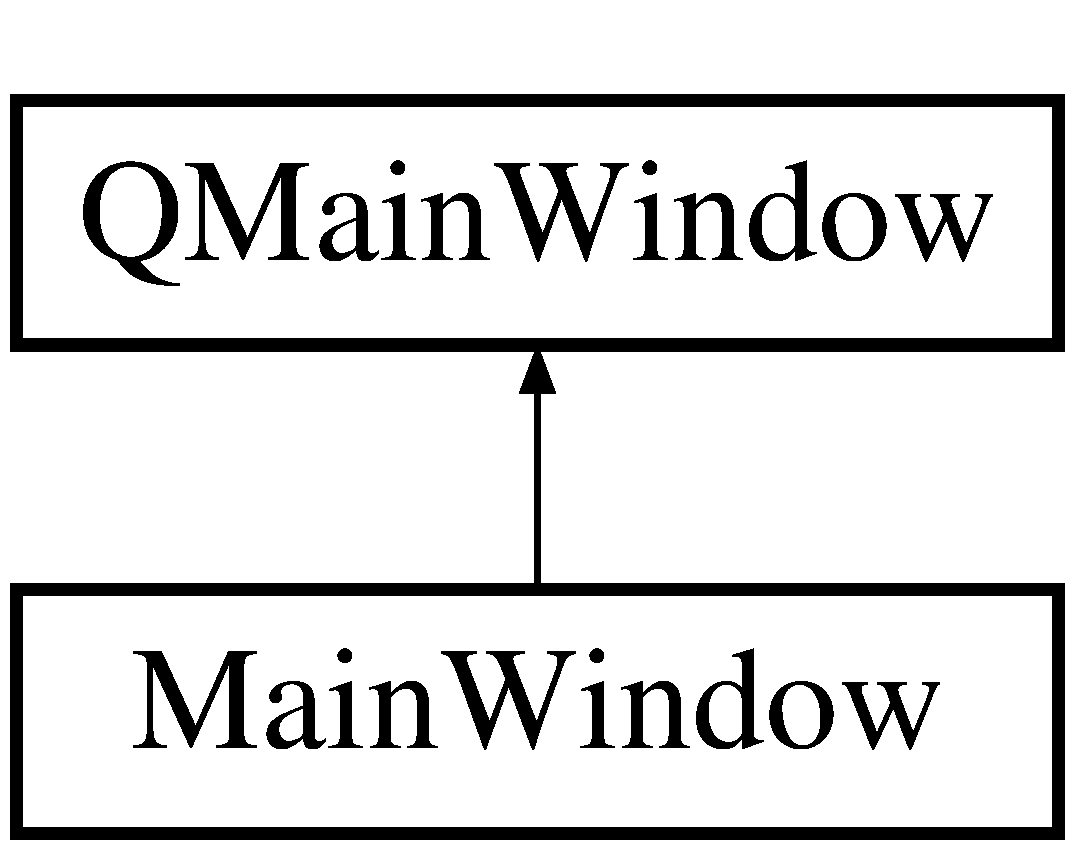
\includegraphics[height=2.000000cm]{class_main_window}
\end{center}
\end{figure}
\subsection*{Public Slots}
\begin{DoxyCompactItemize}
\item 
void \hyperlink{class_main_window_aa760493201dbba331f4447e7b9d7b766}{del\+Scores} ()
\item 
void \hyperlink{class_main_window_a114eef08f156b273538f61c85a3db72f}{reset\+Or\+Not} ()
\item 
void \hyperlink{class_main_window_a04ae3dc178f46ea61ece2b9b209317b8}{cancel} ()
\item 
void \hyperlink{class_main_window_ab1584e555ed5ad91453f18ea51d0351e}{quick\+Game} ()
\item 
void \hyperlink{class_main_window_a36838285112f056c6e8135573918f224}{new\+Game} ()
\item 
void \hyperlink{class_main_window_ae0366468fcf40ee5e65a5239ab530e96}{new\+Game} (int height, int width, int nb\+Col)
\end{DoxyCompactItemize}
\subsection*{Public Member Functions}
\begin{DoxyCompactItemize}
\item 
\hyperlink{class_main_window_a8b244be8b7b7db1b08de2a2acb9409db}{Main\+Window} (Q\+Widget $\ast$parent=0)
\item 
\hyperlink{class_main_window_ae98d00a93bc118200eeef9f9bba1dba7}{$\sim$\+Main\+Window} ()
\end{DoxyCompactItemize}


\subsection{Detailed Description}
The \hyperlink{class_main_window}{Main\+Window} class The application\textquotesingle{}s controller This class manage the different view of the application and the has the game object. 

Definition at line 23 of file mainwindow.\+h.



\subsection{Constructor \& Destructor Documentation}
\hypertarget{class_main_window_a8b244be8b7b7db1b08de2a2acb9409db}{}\label{class_main_window_a8b244be8b7b7db1b08de2a2acb9409db} 
\index{Main\+Window@{Main\+Window}!Main\+Window@{Main\+Window}}
\index{Main\+Window@{Main\+Window}!Main\+Window@{Main\+Window}}
\subsubsection{\texorpdfstring{Main\+Window()}{MainWindow()}}
{\footnotesize\ttfamily Main\+Window\+::\+Main\+Window (\begin{DoxyParamCaption}\item[{Q\+Widget $\ast$}]{parent = {\ttfamily 0} }\end{DoxyParamCaption})\hspace{0.3cm}{\ttfamily [explicit]}}



Definition at line 4 of file mainwindow.\+cpp.


\begin{DoxyCode}
4                                       :
5     QMainWindow(parent),
6     ui(\textcolor{keyword}{new} Ui::MainWindow)
7 \{
8     ui->setupUi(\textcolor{keyword}{this});
9 
10     \_myStack = \textcolor{keyword}{new} QStackedWidget(\textcolor{keyword}{this});
11     \_intro = \textcolor{keyword}{new} \hyperlink{class_intro}{Intro}(\textcolor{keyword}{this});
12     \_menuStart = \textcolor{keyword}{new} \hyperlink{class_menu_start}{MenuStart}(\textcolor{keyword}{this});
13     \_options = \textcolor{keyword}{new} \hyperlink{class_options}{Options}(\textcolor{keyword}{this});
14     \_reset = \textcolor{keyword}{new} \hyperlink{class_reset}{Reset}(\textcolor{keyword}{this});
15     \_myStack->addWidget(\_intro);
16     \_myStack->addWidget(\_menuStart);
17     \_myStack->addWidget(\_options);
18     \_myStack->addWidget(\_reset);
19 
20     this->setCentralWidget(\_myStack);
21     \_myStack->setCurrentIndex(0);
22 
23     QTimer::singleShot(4000, [=]()\{
24         \_myStack->setCurrentIndex(1);
25         setBackground(\textcolor{stringliteral}{":/images/choice.jpg"});
26     \});
27 
28 \}
\end{DoxyCode}
\hypertarget{class_main_window_ae98d00a93bc118200eeef9f9bba1dba7}{}\label{class_main_window_ae98d00a93bc118200eeef9f9bba1dba7} 
\index{Main\+Window@{Main\+Window}!````~Main\+Window@{$\sim$\+Main\+Window}}
\index{````~Main\+Window@{$\sim$\+Main\+Window}!Main\+Window@{Main\+Window}}
\subsubsection{\texorpdfstring{$\sim$\+Main\+Window()}{~MainWindow()}}
{\footnotesize\ttfamily Main\+Window\+::$\sim$\+Main\+Window (\begin{DoxyParamCaption}{ }\end{DoxyParamCaption})}



Definition at line 30 of file mainwindow.\+cpp.


\begin{DoxyCode}
30                        \{
31     \textcolor{keyword}{delete} ui;
32 \}
\end{DoxyCode}


\subsection{Member Function Documentation}
\hypertarget{class_main_window_a04ae3dc178f46ea61ece2b9b209317b8}{}\label{class_main_window_a04ae3dc178f46ea61ece2b9b209317b8} 
\index{Main\+Window@{Main\+Window}!cancel@{cancel}}
\index{cancel@{cancel}!Main\+Window@{Main\+Window}}
\subsubsection{\texorpdfstring{cancel}{cancel}}
{\footnotesize\ttfamily void Main\+Window\+::cancel (\begin{DoxyParamCaption}{ }\end{DoxyParamCaption})\hspace{0.3cm}{\ttfamily [slot]}}



Definition at line 54 of file mainwindow.\+cpp.


\begin{DoxyCode}
54                        \{
55     \_myStack->setCurrentIndex(1);
56     setBackground(\textcolor{stringliteral}{":/images/choice.jpg"});
57 \}
\end{DoxyCode}
\hypertarget{class_main_window_aa760493201dbba331f4447e7b9d7b766}{}\label{class_main_window_aa760493201dbba331f4447e7b9d7b766} 
\index{Main\+Window@{Main\+Window}!del\+Scores@{del\+Scores}}
\index{del\+Scores@{del\+Scores}!Main\+Window@{Main\+Window}}
\subsubsection{\texorpdfstring{del\+Scores}{delScores}}
{\footnotesize\ttfamily void Main\+Window\+::del\+Scores (\begin{DoxyParamCaption}{ }\end{DoxyParamCaption})\hspace{0.3cm}{\ttfamily [slot]}}



Definition at line 72 of file mainwindow.\+cpp.


\begin{DoxyCode}
72                           \{
73     \_myStack->setCurrentIndex(1);
74     setBackground(\textcolor{stringliteral}{":/images/choice.jpg"});
75     \textcolor{keywordflow}{if}( \textcolor{keyword}{remove}( \textcolor{stringliteral}{"save.json"} ) != 0 )
76         perror( \textcolor{stringliteral}{"Error deleting file"} );
77       \textcolor{keywordflow}{else}
78         puts( \textcolor{stringliteral}{"File successfully deleted"} );
79 \}
\end{DoxyCode}
\hypertarget{class_main_window_a36838285112f056c6e8135573918f224}{}\label{class_main_window_a36838285112f056c6e8135573918f224} 
\index{Main\+Window@{Main\+Window}!new\+Game@{new\+Game}}
\index{new\+Game@{new\+Game}!Main\+Window@{Main\+Window}}
\subsubsection{\texorpdfstring{new\+Game}{newGame}\hspace{0.1cm}{\footnotesize\ttfamily [1/2]}}
{\footnotesize\ttfamily void Main\+Window\+::new\+Game (\begin{DoxyParamCaption}{ }\end{DoxyParamCaption})\hspace{0.3cm}{\ttfamily [slot]}}



Definition at line 41 of file mainwindow.\+cpp.


\begin{DoxyCode}
41                         \{
42     \_myStack->setCurrentIndex(2);
43     setBackground(\textcolor{stringliteral}{":/images/options.jpg"});
44 \}
\end{DoxyCode}
\hypertarget{class_main_window_ae0366468fcf40ee5e65a5239ab530e96}{}\label{class_main_window_ae0366468fcf40ee5e65a5239ab530e96} 
\index{Main\+Window@{Main\+Window}!new\+Game@{new\+Game}}
\index{new\+Game@{new\+Game}!Main\+Window@{Main\+Window}}
\subsubsection{\texorpdfstring{new\+Game}{newGame}\hspace{0.1cm}{\footnotesize\ttfamily [2/2]}}
{\footnotesize\ttfamily void Main\+Window\+::new\+Game (\begin{DoxyParamCaption}\item[{int}]{height,  }\item[{int}]{width,  }\item[{int}]{nb\+Col }\end{DoxyParamCaption})\hspace{0.3cm}{\ttfamily [slot]}}



Definition at line 46 of file mainwindow.\+cpp.


\begin{DoxyCode}
46                                                       \{
47 
48     \_wg = \textcolor{keyword}{new} \hyperlink{class_widget_game}{WidgetGame}(height,width,nbCol,\textcolor{keyword}{this});
49     \_myStack->insertWidget(4,\_wg);
50     \_myStack->setCurrentIndex(4);
51     setBackground(\textcolor{stringliteral}{":/images/bluedark.jpg"});
52 \}
\end{DoxyCode}
\hypertarget{class_main_window_ab1584e555ed5ad91453f18ea51d0351e}{}\label{class_main_window_ab1584e555ed5ad91453f18ea51d0351e} 
\index{Main\+Window@{Main\+Window}!quick\+Game@{quick\+Game}}
\index{quick\+Game@{quick\+Game}!Main\+Window@{Main\+Window}}
\subsubsection{\texorpdfstring{quick\+Game}{quickGame}}
{\footnotesize\ttfamily void Main\+Window\+::quick\+Game (\begin{DoxyParamCaption}{ }\end{DoxyParamCaption})\hspace{0.3cm}{\ttfamily [slot]}}



Definition at line 34 of file mainwindow.\+cpp.


\begin{DoxyCode}
34                           \{
35     \_wg = \textcolor{keyword}{new} \hyperlink{class_widget_game}{WidgetGame}(15,15,4,\textcolor{keyword}{this});
36     \_myStack->insertWidget(4,\_wg);
37     \_myStack->setCurrentIndex(4);
38     setBackground(\textcolor{stringliteral}{":/images/bluedark.jpg"});
39 \}
\end{DoxyCode}
\hypertarget{class_main_window_a114eef08f156b273538f61c85a3db72f}{}\label{class_main_window_a114eef08f156b273538f61c85a3db72f} 
\index{Main\+Window@{Main\+Window}!reset\+Or\+Not@{reset\+Or\+Not}}
\index{reset\+Or\+Not@{reset\+Or\+Not}!Main\+Window@{Main\+Window}}
\subsubsection{\texorpdfstring{reset\+Or\+Not}{resetOrNot}}
{\footnotesize\ttfamily void Main\+Window\+::reset\+Or\+Not (\begin{DoxyParamCaption}{ }\end{DoxyParamCaption})\hspace{0.3cm}{\ttfamily [slot]}}



Definition at line 67 of file mainwindow.\+cpp.


\begin{DoxyCode}
67                            \{
68     \_myStack->setCurrentIndex(3);
69     setBackground(\textcolor{stringliteral}{":/images/reset.jpg"});
70 \}
\end{DoxyCode}


The documentation for this class was generated from the following files\+:\begin{DoxyCompactItemize}
\item 
view/\hyperlink{mainwindow_8h}{mainwindow.\+h}\item 
view/\hyperlink{mainwindow_8cpp}{mainwindow.\+cpp}\end{DoxyCompactItemize}

\hypertarget{class_menu_start}{}\section{Menu\+Start Class Reference}
\label{class_menu_start}\index{Menu\+Start@{Menu\+Start}}


The \hyperlink{class_menu_start}{Menu\+Start} class To let the choice between a new game or a quickgame.  




{\ttfamily \#include $<$menustart.\+h$>$}

Inheritance diagram for Menu\+Start\+:\begin{figure}[H]
\begin{center}
\leavevmode
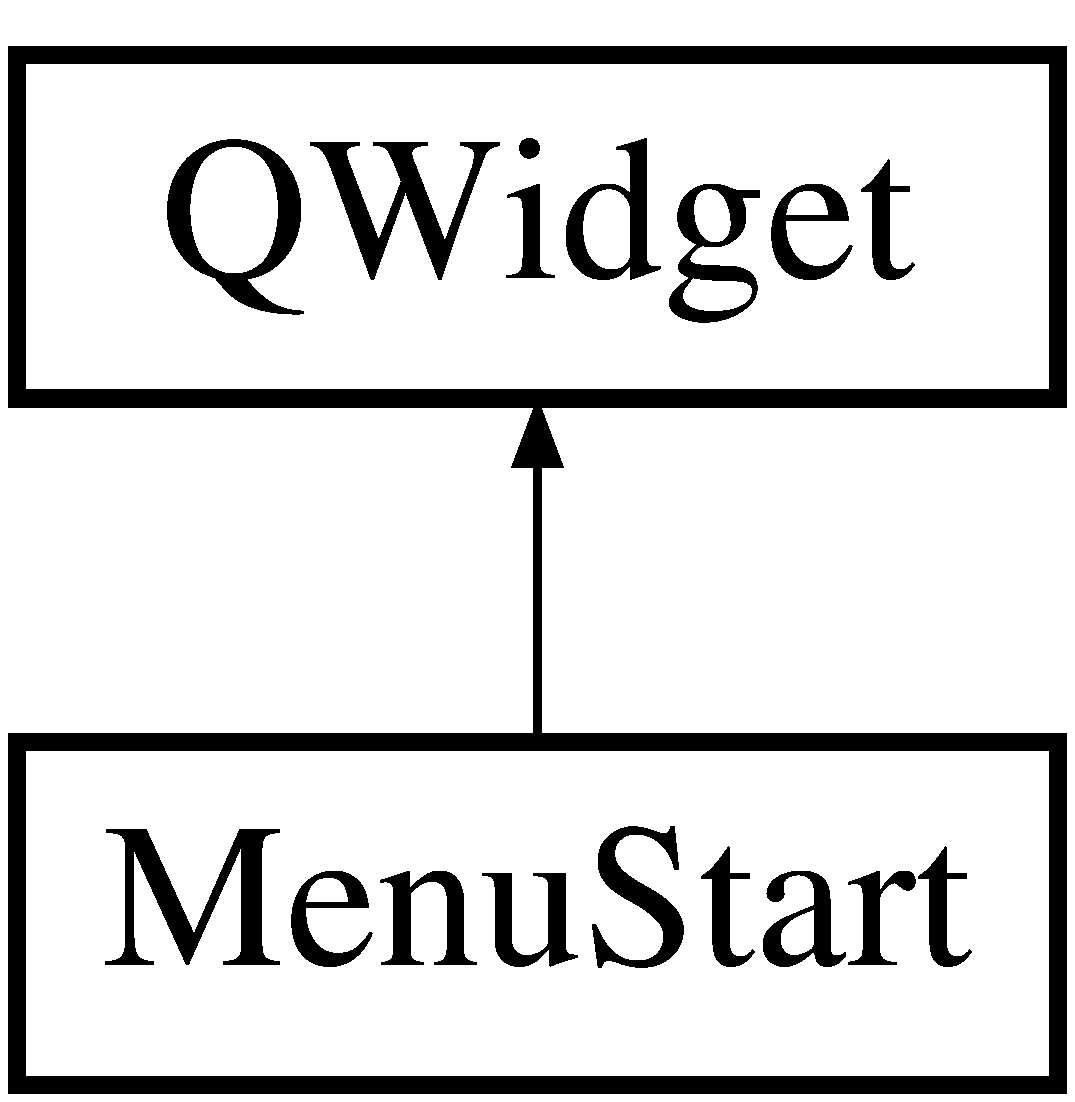
\includegraphics[height=2.000000cm]{class_menu_start}
\end{center}
\end{figure}
\subsection*{Public Member Functions}
\begin{DoxyCompactItemize}
\item 
\hyperlink{class_menu_start_a184ff65bb2534378670fee22487b02eb}{Menu\+Start} (Q\+Widget $\ast$parent=0)
\item 
\hyperlink{class_menu_start_a3c8fe892ee7171d64a9857f44ad326ba}{$\sim$\+Menu\+Start} ()
\end{DoxyCompactItemize}


\subsection{Detailed Description}
The \hyperlink{class_menu_start}{Menu\+Start} class To let the choice between a new game or a quickgame. 

Definition at line 16 of file menustart.\+h.



\subsection{Constructor \& Destructor Documentation}
\hypertarget{class_menu_start_a184ff65bb2534378670fee22487b02eb}{}\label{class_menu_start_a184ff65bb2534378670fee22487b02eb} 
\index{Menu\+Start@{Menu\+Start}!Menu\+Start@{Menu\+Start}}
\index{Menu\+Start@{Menu\+Start}!Menu\+Start@{Menu\+Start}}
\subsubsection{\texorpdfstring{Menu\+Start()}{MenuStart()}}
{\footnotesize\ttfamily Menu\+Start\+::\+Menu\+Start (\begin{DoxyParamCaption}\item[{Q\+Widget $\ast$}]{parent = {\ttfamily 0} }\end{DoxyParamCaption})\hspace{0.3cm}{\ttfamily [explicit]}}



Definition at line 3 of file menustart.\+cpp.


\begin{DoxyCode}
3                                     :
4     QWidget(parent)
5 \{
6     QVBoxLayout *qvb = \textcolor{keyword}{new} QVBoxLayout();
7     QPushButton *quick = \textcolor{keyword}{new} QPushButton(\textcolor{stringliteral}{"Quick Game"});
8     QPushButton *newGame = \textcolor{keyword}{new} QPushButton(\textcolor{stringliteral}{"New Game"});
9     QPushButton *reset = \textcolor{keyword}{new} QPushButton(\textcolor{stringliteral}{"Reset scores"});
10 
11     connect(quick,SIGNAL(clicked()),parent,SLOT(quickGame()));
12     connect(newGame,SIGNAL(clicked()),parent,SLOT(newGame()));
13     connect(reset,SIGNAL(clicked()),parent,SLOT(resetOrNot()));
14 
15     quick->setSizePolicy(QSizePolicy::Fixed,QSizePolicy::Fixed);
16     newGame->setSizePolicy(QSizePolicy::Fixed,QSizePolicy::Fixed);
17     reset->setSizePolicy(QSizePolicy::Fixed,QSizePolicy::Fixed);
18 
19     qvb->addWidget(quick);
20     qvb->addWidget(newGame);
21     qvb->addWidget(reset);
22     qvb->setMargin(250);
23     qvb->setAlignment(quick,Qt::AlignCenter);
24     qvb->setAlignment(newGame,Qt::AlignCenter);
25     qvb->setAlignment(reset,Qt::AlignCenter);
26     setLayout(qvb);
27 \}
\end{DoxyCode}
\hypertarget{class_menu_start_a3c8fe892ee7171d64a9857f44ad326ba}{}\label{class_menu_start_a3c8fe892ee7171d64a9857f44ad326ba} 
\index{Menu\+Start@{Menu\+Start}!````~Menu\+Start@{$\sim$\+Menu\+Start}}
\index{````~Menu\+Start@{$\sim$\+Menu\+Start}!Menu\+Start@{Menu\+Start}}
\subsubsection{\texorpdfstring{$\sim$\+Menu\+Start()}{~MenuStart()}}
{\footnotesize\ttfamily Menu\+Start\+::$\sim$\+Menu\+Start (\begin{DoxyParamCaption}{ }\end{DoxyParamCaption})}



Definition at line 29 of file menustart.\+cpp.


\begin{DoxyCode}
29 \{\}
\end{DoxyCode}


The documentation for this class was generated from the following files\+:\begin{DoxyCompactItemize}
\item 
view/\hyperlink{menustart_8h}{menustart.\+h}\item 
view/\hyperlink{menustart_8cpp}{menustart.\+cpp}\end{DoxyCompactItemize}

\hypertarget{classoli_1_1_observable}{}\section{oli\+:\+:Observable Class Reference}
\label{classoli_1_1_observable}\index{oli\+::\+Observable@{oli\+::\+Observable}}


The \hyperlink{classoli_1_1_observable}{Observable} class Interface implemented by the classes that have to be observed.  




{\ttfamily \#include $<$observable.\+h$>$}

Inheritance diagram for oli\+:\+:Observable\+:\begin{figure}[H]
\begin{center}
\leavevmode
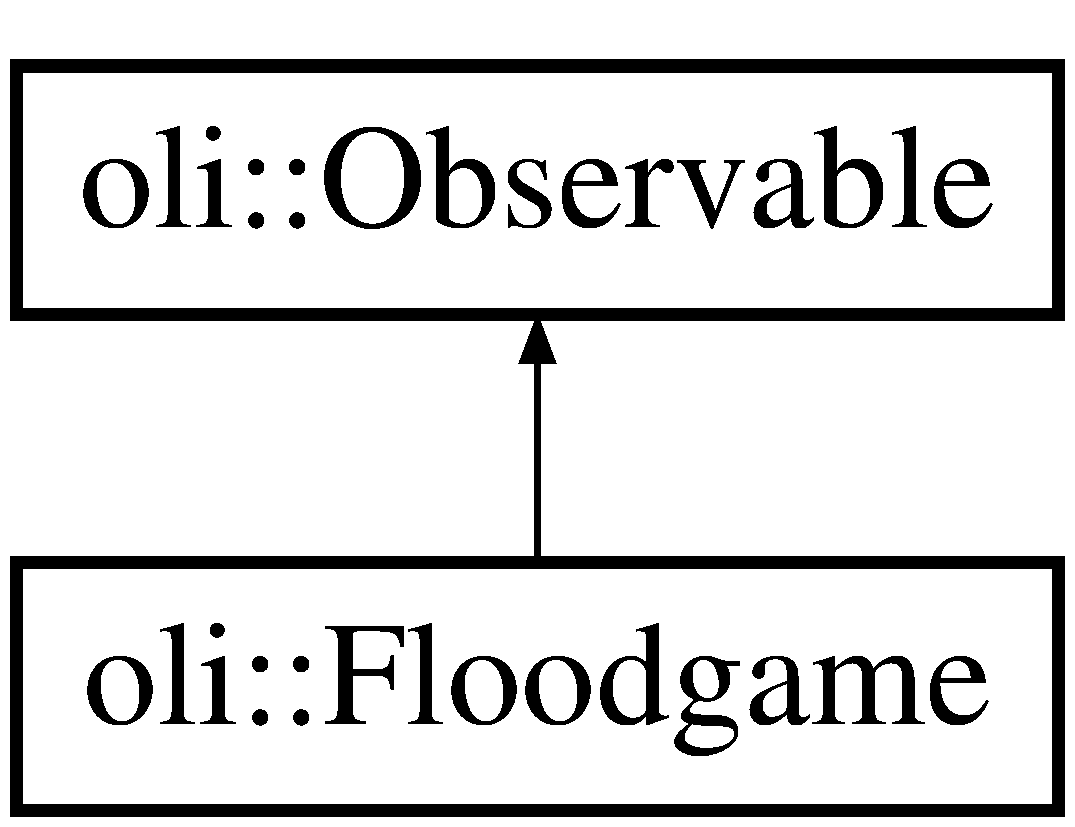
\includegraphics[height=2.000000cm]{classoli_1_1_observable}
\end{center}
\end{figure}
\subsection*{Public Member Functions}
\begin{DoxyCompactItemize}
\item 
void \hyperlink{classoli_1_1_observable_af746a8f49e2b08bc93767281dd813532}{Add\+Obs} (\hyperlink{classoli_1_1_observer}{Observer} $\ast$obs)
\item 
void \hyperlink{classoli_1_1_observable_a9fb13016d9b81c1132171b581e243d8b}{Del\+Obs} (\hyperlink{classoli_1_1_observer}{Observer} $\ast$obs)
\item 
void \hyperlink{classoli_1_1_observable_ab1fe0a40f7aaa9d9acee97f8c08ec328}{Notify} (void)
\item 
virtual \hyperlink{classoli_1_1_observable_aabeb2ecf331c7ecb274594df6f4e82b1}{$\sim$\+Observable} ()
\end{DoxyCompactItemize}


\subsection{Detailed Description}
The \hyperlink{classoli_1_1_observable}{Observable} class Interface implemented by the classes that have to be observed. 

Definition at line 12 of file observable.\+h.



\subsection{Constructor \& Destructor Documentation}
\hypertarget{classoli_1_1_observable_aabeb2ecf331c7ecb274594df6f4e82b1}{}\label{classoli_1_1_observable_aabeb2ecf331c7ecb274594df6f4e82b1} 
\index{oli\+::\+Observable@{oli\+::\+Observable}!````~Observable@{$\sim$\+Observable}}
\index{````~Observable@{$\sim$\+Observable}!oli\+::\+Observable@{oli\+::\+Observable}}
\subsubsection{\texorpdfstring{$\sim$\+Observable()}{~Observable()}}
{\footnotesize\ttfamily oli\+::\+Observable\+::$\sim$\+Observable (\begin{DoxyParamCaption}{ }\end{DoxyParamCaption})\hspace{0.3cm}{\ttfamily [virtual]}}



Definition at line 17 of file observable.\+cpp.


\begin{DoxyCode}
17                        \{
18     iterator itb=m\_list.begin();
19     const\_iterator ite=m\_list.end();
20 
21     \textcolor{keywordflow}{for}(;itb!=ite;++itb)\{
22         (*itb)->DelObs(\textcolor{keyword}{this});
23     \}
24 \}
\end{DoxyCode}


\subsection{Member Function Documentation}
\hypertarget{classoli_1_1_observable_af746a8f49e2b08bc93767281dd813532}{}\label{classoli_1_1_observable_af746a8f49e2b08bc93767281dd813532} 
\index{oli\+::\+Observable@{oli\+::\+Observable}!Add\+Obs@{Add\+Obs}}
\index{Add\+Obs@{Add\+Obs}!oli\+::\+Observable@{oli\+::\+Observable}}
\subsubsection{\texorpdfstring{Add\+Obs()}{AddObs()}}
{\footnotesize\ttfamily void oli\+::\+Observable\+::\+Add\+Obs (\begin{DoxyParamCaption}\item[{\hyperlink{classoli_1_1_observer}{Observer} $\ast$}]{obs }\end{DoxyParamCaption})}



Definition at line 6 of file observable.\+cpp.


\begin{DoxyCode}
6                                      \{
7     m\_list.push\_back(obs);
8     obs->AddObs(\textcolor{keyword}{this});
9 \}
\end{DoxyCode}
\hypertarget{classoli_1_1_observable_a9fb13016d9b81c1132171b581e243d8b}{}\label{classoli_1_1_observable_a9fb13016d9b81c1132171b581e243d8b} 
\index{oli\+::\+Observable@{oli\+::\+Observable}!Del\+Obs@{Del\+Obs}}
\index{Del\+Obs@{Del\+Obs}!oli\+::\+Observable@{oli\+::\+Observable}}
\subsubsection{\texorpdfstring{Del\+Obs()}{DelObs()}}
{\footnotesize\ttfamily void oli\+::\+Observable\+::\+Del\+Obs (\begin{DoxyParamCaption}\item[{\hyperlink{classoli_1_1_observer}{Observer} $\ast$}]{obs }\end{DoxyParamCaption})}



Definition at line 11 of file observable.\+cpp.


\begin{DoxyCode}
11                                     \{
12     iterator it= find(m\_list.begin(),m\_list.end(),obs);
13     \textcolor{keywordflow}{if}(it != m\_list.end())
14         m\_list.erase(it);
15 \}
\end{DoxyCode}
\hypertarget{classoli_1_1_observable_ab1fe0a40f7aaa9d9acee97f8c08ec328}{}\label{classoli_1_1_observable_ab1fe0a40f7aaa9d9acee97f8c08ec328} 
\index{oli\+::\+Observable@{oli\+::\+Observable}!Notify@{Notify}}
\index{Notify@{Notify}!oli\+::\+Observable@{oli\+::\+Observable}}
\subsubsection{\texorpdfstring{Notify()}{Notify()}}
{\footnotesize\ttfamily void oli\+::\+Observable\+::\+Notify (\begin{DoxyParamCaption}\item[{void}]{ }\end{DoxyParamCaption})}



Definition at line 26 of file observable.\+cpp.


\begin{DoxyCode}
26                            \{
27     iterator itb=m\_list.begin();
28     const\_iterator ite=m\_list.end();
29 
30     \textcolor{keywordflow}{for}(;itb!=ite;++itb)\{
31         (*itb)->Update();
32     \}
33 \}
\end{DoxyCode}


The documentation for this class was generated from the following files\+:\begin{DoxyCompactItemize}
\item 
observer/\hyperlink{observable_8h}{observable.\+h}\item 
observer/\hyperlink{observable_8cpp}{observable.\+cpp}\end{DoxyCompactItemize}

\hypertarget{classoli_1_1_observer}{}\section{oli\+:\+:Observer Class Reference}
\label{classoli_1_1_observer}\index{oli\+::\+Observer@{oli\+::\+Observer}}


The \hyperlink{classoli_1_1_observer}{Observer} class Implemented by the class that have to Observe another class(observable)  




{\ttfamily \#include $<$observer.\+h$>$}

Inheritance diagram for oli\+:\+:Observer\+:\begin{figure}[H]
\begin{center}
\leavevmode
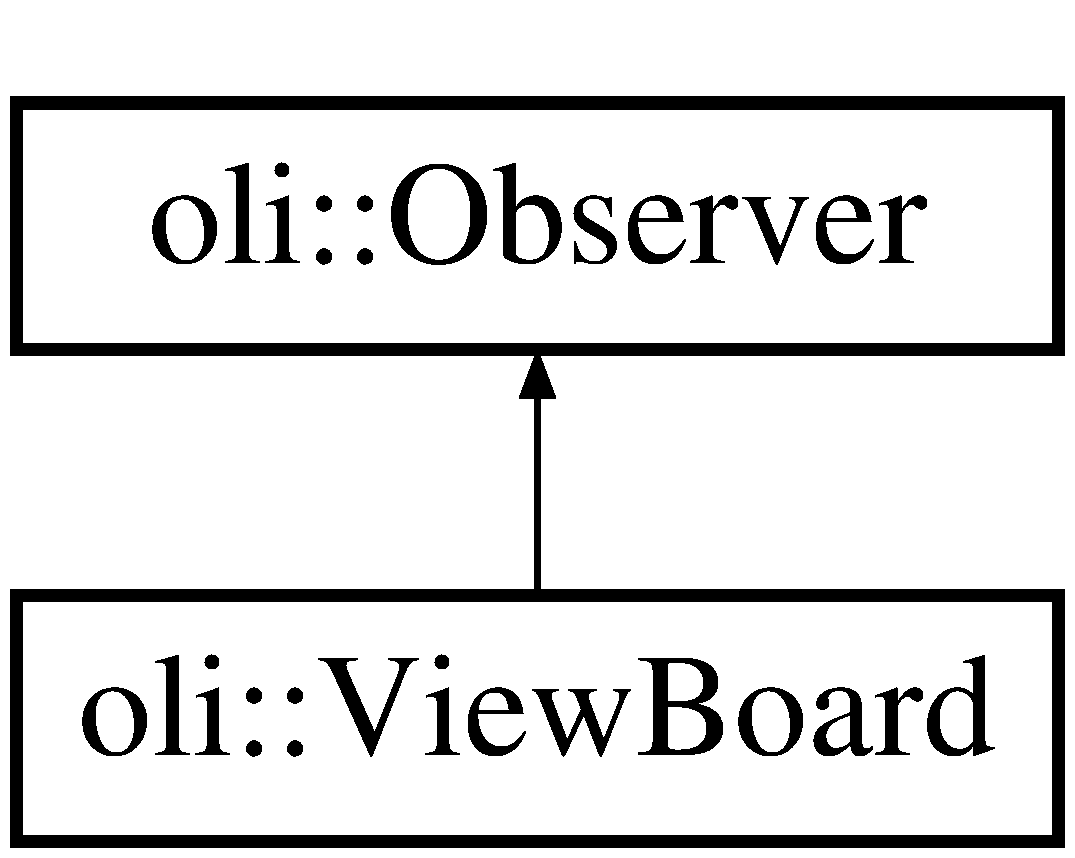
\includegraphics[height=2.000000cm]{classoli_1_1_observer}
\end{center}
\end{figure}
\subsection*{Public Member Functions}
\begin{DoxyCompactItemize}
\item 
virtual void \hyperlink{classoli_1_1_observer_a81154a42166f88a6e341909438a07b75}{Update} ()=0
\item 
void \hyperlink{classoli_1_1_observer_a3d6dbe2f29de6f9aa33fcabe7d42d90c}{Add\+Obs} (\hyperlink{classoli_1_1_observable}{Observable} $\ast$obs)
\item 
void \hyperlink{classoli_1_1_observer_af34e52ebb941e7be3c1f1decd4299548}{Del\+Obs} (\hyperlink{classoli_1_1_observable}{Observable} $\ast$obs)
\end{DoxyCompactItemize}
\subsection*{Protected Types}
\begin{DoxyCompactItemize}
\item 
typedef std\+::list$<$ \hyperlink{classoli_1_1_observable}{Observable} $\ast$ $>$\+::\hyperlink{classoli_1_1_observer_a845b9aed78746c4f413cdeae346ca1b3}{iterator} \hyperlink{classoli_1_1_observer_a845b9aed78746c4f413cdeae346ca1b3}{iterator}
\item 
typedef std\+::list$<$ \hyperlink{classoli_1_1_observable}{Observable} $\ast$ $>$\+::\hyperlink{classoli_1_1_observer_a1b49363f9c8afdb6734aa28d685579ef}{const\+\_\+iterator} \hyperlink{classoli_1_1_observer_a1b49363f9c8afdb6734aa28d685579ef}{const\+\_\+iterator}
\end{DoxyCompactItemize}
\subsection*{Protected Member Functions}
\begin{DoxyCompactItemize}
\item 
virtual \hyperlink{classoli_1_1_observer_a204c75941c51c46cf8930361d8948939}{$\sim$\+Observer} ()=0
\end{DoxyCompactItemize}
\subsection*{Protected Attributes}
\begin{DoxyCompactItemize}
\item 
std\+::list$<$ \hyperlink{classoli_1_1_observable}{Observable} $\ast$ $>$ \hyperlink{classoli_1_1_observer_acf615598b1c72e779d12c8b9b9422c86}{m\+\_\+list}
\end{DoxyCompactItemize}


\subsection{Detailed Description}
The \hyperlink{classoli_1_1_observer}{Observer} class Implemented by the class that have to Observe another class(observable) 

Definition at line 17 of file observer.\+h.



\subsection{Member Typedef Documentation}
\hypertarget{classoli_1_1_observer_a1b49363f9c8afdb6734aa28d685579ef}{}\label{classoli_1_1_observer_a1b49363f9c8afdb6734aa28d685579ef} 
\index{oli\+::\+Observer@{oli\+::\+Observer}!const\+\_\+iterator@{const\+\_\+iterator}}
\index{const\+\_\+iterator@{const\+\_\+iterator}!oli\+::\+Observer@{oli\+::\+Observer}}
\subsubsection{\texorpdfstring{const\+\_\+iterator}{const\_iterator}}
{\footnotesize\ttfamily typedef std\+::list$<$\hyperlink{classoli_1_1_observable}{Observable}$\ast$$>$\+::\hyperlink{classoli_1_1_observer_a1b49363f9c8afdb6734aa28d685579ef}{const\+\_\+iterator} \hyperlink{classoli_1_1_observer_a1b49363f9c8afdb6734aa28d685579ef}{oli\+::\+Observer\+::const\+\_\+iterator}\hspace{0.3cm}{\ttfamily [protected]}}



Definition at line 22 of file observer.\+h.

\hypertarget{classoli_1_1_observer_a845b9aed78746c4f413cdeae346ca1b3}{}\label{classoli_1_1_observer_a845b9aed78746c4f413cdeae346ca1b3} 
\index{oli\+::\+Observer@{oli\+::\+Observer}!iterator@{iterator}}
\index{iterator@{iterator}!oli\+::\+Observer@{oli\+::\+Observer}}
\subsubsection{\texorpdfstring{iterator}{iterator}}
{\footnotesize\ttfamily typedef std\+::list$<$\hyperlink{classoli_1_1_observable}{Observable}$\ast$$>$\+::\hyperlink{classoli_1_1_observer_a845b9aed78746c4f413cdeae346ca1b3}{iterator} \hyperlink{classoli_1_1_observer_a845b9aed78746c4f413cdeae346ca1b3}{oli\+::\+Observer\+::iterator}\hspace{0.3cm}{\ttfamily [protected]}}



Definition at line 21 of file observer.\+h.



\subsection{Constructor \& Destructor Documentation}
\hypertarget{classoli_1_1_observer_a204c75941c51c46cf8930361d8948939}{}\label{classoli_1_1_observer_a204c75941c51c46cf8930361d8948939} 
\index{oli\+::\+Observer@{oli\+::\+Observer}!````~Observer@{$\sim$\+Observer}}
\index{````~Observer@{$\sim$\+Observer}!oli\+::\+Observer@{oli\+::\+Observer}}
\subsubsection{\texorpdfstring{$\sim$\+Observer()}{~Observer()}}
{\footnotesize\ttfamily oli\+::\+Observer\+::$\sim$\+Observer (\begin{DoxyParamCaption}{ }\end{DoxyParamCaption})\hspace{0.3cm}{\ttfamily [protected]}, {\ttfamily [pure virtual]}}



Definition at line 11 of file observer.\+cpp.


\begin{DoxyCode}
11                    \{
12 
13     \hyperlink{classoli_1_1_observer_a1b49363f9c8afdb6734aa28d685579ef}{const\_iterator} ite=\hyperlink{classoli_1_1_observer_acf615598b1c72e779d12c8b9b9422c86}{m\_list}.end();
14 
15     \textcolor{keywordflow}{for}(\hyperlink{classoli_1_1_observer_a845b9aed78746c4f413cdeae346ca1b3}{iterator} itb=\hyperlink{classoli_1_1_observer_acf615598b1c72e779d12c8b9b9422c86}{m\_list}.begin();itb!=ite;++itb)\{
16         (*itb)->DelObs(\textcolor{keyword}{this});
17     \}
18 \}
\end{DoxyCode}


\subsection{Member Function Documentation}
\hypertarget{classoli_1_1_observer_a3d6dbe2f29de6f9aa33fcabe7d42d90c}{}\label{classoli_1_1_observer_a3d6dbe2f29de6f9aa33fcabe7d42d90c} 
\index{oli\+::\+Observer@{oli\+::\+Observer}!Add\+Obs@{Add\+Obs}}
\index{Add\+Obs@{Add\+Obs}!oli\+::\+Observer@{oli\+::\+Observer}}
\subsubsection{\texorpdfstring{Add\+Obs()}{AddObs()}}
{\footnotesize\ttfamily void oli\+::\+Observer\+::\+Add\+Obs (\begin{DoxyParamCaption}\item[{\hyperlink{classoli_1_1_observable}{Observable} $\ast$}]{obs }\end{DoxyParamCaption})}



Definition at line 20 of file observer.\+cpp.


\begin{DoxyCode}
20                                      \{
21     \hyperlink{classoli_1_1_observer_acf615598b1c72e779d12c8b9b9422c86}{m\_list}.push\_back(obs);
22 \}
\end{DoxyCode}
\hypertarget{classoli_1_1_observer_af34e52ebb941e7be3c1f1decd4299548}{}\label{classoli_1_1_observer_af34e52ebb941e7be3c1f1decd4299548} 
\index{oli\+::\+Observer@{oli\+::\+Observer}!Del\+Obs@{Del\+Obs}}
\index{Del\+Obs@{Del\+Obs}!oli\+::\+Observer@{oli\+::\+Observer}}
\subsubsection{\texorpdfstring{Del\+Obs()}{DelObs()}}
{\footnotesize\ttfamily void oli\+::\+Observer\+::\+Del\+Obs (\begin{DoxyParamCaption}\item[{\hyperlink{classoli_1_1_observable}{Observable} $\ast$}]{obs }\end{DoxyParamCaption})}



Definition at line 24 of file observer.\+cpp.


\begin{DoxyCode}
24                                     \{
25 
26     \hyperlink{classoli_1_1_observer_a845b9aed78746c4f413cdeae346ca1b3}{iterator} it= std::find(\hyperlink{classoli_1_1_observer_acf615598b1c72e779d12c8b9b9422c86}{m\_list}.begin(),\hyperlink{classoli_1_1_observer_acf615598b1c72e779d12c8b9b9422c86}{m\_list}.end(),obs);
27     \textcolor{keywordflow}{if}(it != \hyperlink{classoli_1_1_observer_acf615598b1c72e779d12c8b9b9422c86}{m\_list}.end())
28         \hyperlink{classoli_1_1_observer_acf615598b1c72e779d12c8b9b9422c86}{m\_list}.erase(it);
29 \}
\end{DoxyCode}
\hypertarget{classoli_1_1_observer_a81154a42166f88a6e341909438a07b75}{}\label{classoli_1_1_observer_a81154a42166f88a6e341909438a07b75} 
\index{oli\+::\+Observer@{oli\+::\+Observer}!Update@{Update}}
\index{Update@{Update}!oli\+::\+Observer@{oli\+::\+Observer}}
\subsubsection{\texorpdfstring{Update()}{Update()}}
{\footnotesize\ttfamily virtual void oli\+::\+Observer\+::\+Update (\begin{DoxyParamCaption}{ }\end{DoxyParamCaption})\hspace{0.3cm}{\ttfamily [pure virtual]}}



Implemented in \hyperlink{classoli_1_1_view_board_a487ea5886ec5de0422fc6e060aa7045b}{oli\+::\+View\+Board}.



\subsection{Member Data Documentation}
\hypertarget{classoli_1_1_observer_acf615598b1c72e779d12c8b9b9422c86}{}\label{classoli_1_1_observer_acf615598b1c72e779d12c8b9b9422c86} 
\index{oli\+::\+Observer@{oli\+::\+Observer}!m\+\_\+list@{m\+\_\+list}}
\index{m\+\_\+list@{m\+\_\+list}!oli\+::\+Observer@{oli\+::\+Observer}}
\subsubsection{\texorpdfstring{m\+\_\+list}{m\_list}}
{\footnotesize\ttfamily std\+::list$<$\hyperlink{classoli_1_1_observable}{Observable}$\ast$$>$ oli\+::\+Observer\+::m\+\_\+list\hspace{0.3cm}{\ttfamily [protected]}}



Definition at line 20 of file observer.\+h.



The documentation for this class was generated from the following files\+:\begin{DoxyCompactItemize}
\item 
observer/\hyperlink{observer_8h}{observer.\+h}\item 
observer/\hyperlink{observer_8cpp}{observer.\+cpp}\end{DoxyCompactItemize}

\hypertarget{class_options}{}\section{Options Class Reference}
\label{class_options}\index{Options@{Options}}


The \hyperlink{class_options}{Options} class the class that make possible to change new game\textquotesingle{}s options.  




{\ttfamily \#include $<$options.\+h$>$}

Inheritance diagram for Options\+:\begin{figure}[H]
\begin{center}
\leavevmode
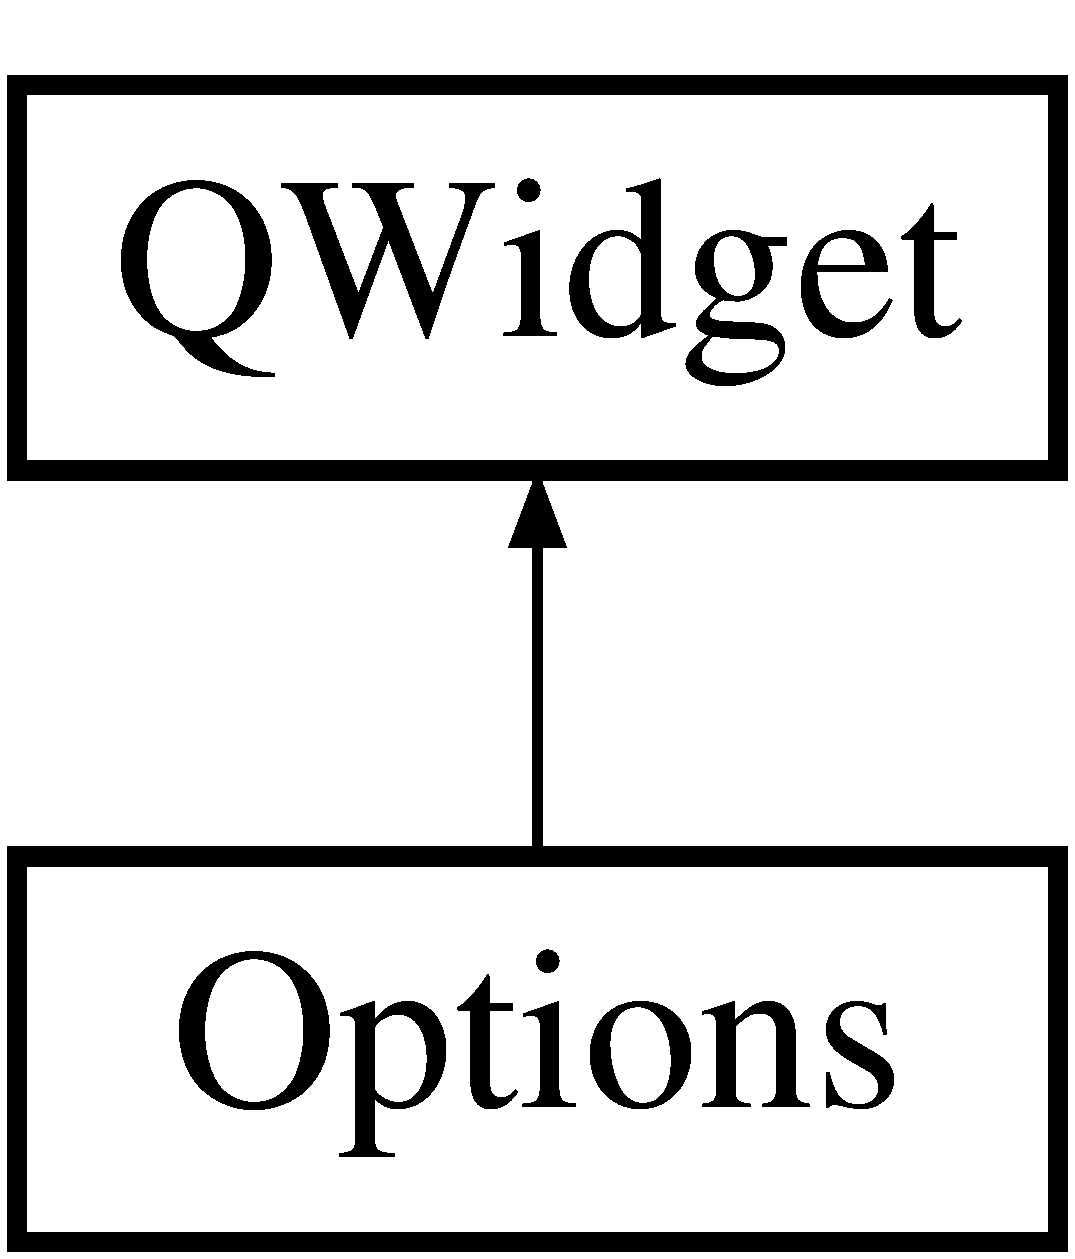
\includegraphics[height=2.000000cm]{class_options}
\end{center}
\end{figure}
\subsection*{Signals}
\begin{DoxyCompactItemize}
\item 
void \hyperlink{class_options_aebc534fbc72d1be99b44fdd691d10ebc}{options} (int height, int width, int nb\+Col)
\end{DoxyCompactItemize}
\subsection*{Public Member Functions}
\begin{DoxyCompactItemize}
\item 
\hyperlink{class_options_a87403ad1d6bd9ae2b54af860bb0f0952}{Options} (Q\+Widget $\ast$parent=0)
\item 
\hyperlink{class_options_a86ddb85b183f8b58af5481f30a42fa92}{$\sim$\+Options} ()
\end{DoxyCompactItemize}


\subsection{Detailed Description}
The \hyperlink{class_options}{Options} class the class that make possible to change new game\textquotesingle{}s options. 

Definition at line 18 of file options.\+h.



\subsection{Constructor \& Destructor Documentation}
\hypertarget{class_options_a87403ad1d6bd9ae2b54af860bb0f0952}{}\label{class_options_a87403ad1d6bd9ae2b54af860bb0f0952} 
\index{Options@{Options}!Options@{Options}}
\index{Options@{Options}!Options@{Options}}
\subsubsection{\texorpdfstring{Options()}{Options()}}
{\footnotesize\ttfamily Options\+::\+Options (\begin{DoxyParamCaption}\item[{Q\+Widget $\ast$}]{parent = {\ttfamily 0} }\end{DoxyParamCaption})\hspace{0.3cm}{\ttfamily [explicit]}}



Definition at line 3 of file options.\+cpp.


\begin{DoxyCode}
3                                 :
4     QWidget(parent)
5 \{
6     QVBoxLayout *boxAll = \textcolor{keyword}{new} QVBoxLayout();
7     QHBoxLayout *boxSize = \textcolor{keyword}{new} QHBoxLayout();
8     QHBoxLayout *boxWidth = \textcolor{keyword}{new} QHBoxLayout();
9 
10 
11     QLabel *width = \textcolor{keyword}{new} QLabel(\textcolor{stringliteral}{"width"});
12 
13     QHBoxLayout *boxHeight = \textcolor{keyword}{new} QHBoxLayout();
14     QLabel *height = \textcolor{keyword}{new} QLabel(\textcolor{stringliteral}{"height"});
15     QHBoxLayout *boxColors = \textcolor{keyword}{new} QHBoxLayout();
16     QLabel *nbColors = \textcolor{keyword}{new} QLabel(\textcolor{stringliteral}{"Number of colors"});
17     QPushButton *start = \textcolor{keyword}{new} QPushButton(\textcolor{stringliteral}{"Start"});
18     QPushButton *cancel = \textcolor{keyword}{new} QPushButton(\textcolor{stringliteral}{"Cancel"});
19 
20     \_spinWidth = \textcolor{keyword}{new} QSpinBox();
21     \_spinWidth->setRange(5,35);
22     \_spinWidth->setValue(10);
23 
24     \_spinHeight = \textcolor{keyword}{new} QSpinBox();
25     \_spinHeight->setRange(5,35);
26     \_spinHeight->setValue(10);
27 
28     \_spinColors = \textcolor{keyword}{new} QSpinBox();
29     \_spinColors->setRange(2,8);
30     \_spinColors->setValue(4);
31 
32     width->setStyleSheet(\textcolor{stringliteral}{"QLabel \{ background-color : transparent; color : white; \}"});
33     height->setStyleSheet(\textcolor{stringliteral}{"QLabel \{ background-color : transparent; color : white; \}"});
34     nbColors->setStyleSheet(\textcolor{stringliteral}{"QLabel \{ background-color : transparent; color : white; \}"});
35 
36     start->setSizePolicy(QSizePolicy::Fixed,QSizePolicy::Fixed);
37     cancel->setSizePolicy(QSizePolicy::Fixed,QSizePolicy::Fixed);
38 
39     connect(cancel,SIGNAL(clicked()),parent,SLOT(cancel()));
40     connect(start,SIGNAL(clicked()),\textcolor{keyword}{this},SLOT(reemitOptions()));
41 
42     boxWidth->addWidget(width);
43     boxWidth->addWidget(\_spinWidth);
44 
45     boxWidth->addWidget(height);
46     boxWidth->addWidget(\_spinHeight);
47 
48     boxSize->addLayout(boxWidth);
49     boxSize->addLayout(boxHeight);
50 
51     boxColors->addWidget(nbColors);
52     boxColors->addWidget(\_spinColors);
53 
54     boxAll->addLayout(boxSize);
55     boxAll->addLayout(boxColors);
56     boxAll->addWidget(start);
57     boxAll->addWidget(cancel);
58 
59     boxAll->setAlignment(start,Qt::AlignCenter);
60     boxAll->setAlignment(cancel,Qt::AlignCenter);
61     boxAll->setAlignment(Qt::AlignCenter);
62     boxAll->setMargin(240);
63 
64     setLayout(boxAll);
65 
66     connect(\textcolor{keyword}{this},(SIGNAL(\hyperlink{class_options_aebc534fbc72d1be99b44fdd691d10ebc}{options}(\textcolor{keywordtype}{int},\textcolor{keywordtype}{int},\textcolor{keywordtype}{int}))),parent,SLOT(newGame(\textcolor{keywordtype}{int},\textcolor{keywordtype}{int},\textcolor{keywordtype}{int})));
67 \}
\end{DoxyCode}
\hypertarget{class_options_a86ddb85b183f8b58af5481f30a42fa92}{}\label{class_options_a86ddb85b183f8b58af5481f30a42fa92} 
\index{Options@{Options}!````~Options@{$\sim$\+Options}}
\index{````~Options@{$\sim$\+Options}!Options@{Options}}
\subsubsection{\texorpdfstring{$\sim$\+Options()}{~Options()}}
{\footnotesize\ttfamily Options\+::$\sim$\+Options (\begin{DoxyParamCaption}{ }\end{DoxyParamCaption})}



Definition at line 69 of file options.\+cpp.


\begin{DoxyCode}
69 \{\}
\end{DoxyCode}


\subsection{Member Function Documentation}
\hypertarget{class_options_aebc534fbc72d1be99b44fdd691d10ebc}{}\label{class_options_aebc534fbc72d1be99b44fdd691d10ebc} 
\index{Options@{Options}!options@{options}}
\index{options@{options}!Options@{Options}}
\subsubsection{\texorpdfstring{options}{options}}
{\footnotesize\ttfamily void Options\+::options (\begin{DoxyParamCaption}\item[{int}]{height,  }\item[{int}]{width,  }\item[{int}]{nb\+Col }\end{DoxyParamCaption})\hspace{0.3cm}{\ttfamily [signal]}}



The documentation for this class was generated from the following files\+:\begin{DoxyCompactItemize}
\item 
view/\hyperlink{options_8h}{options.\+h}\item 
view/\hyperlink{options_8cpp}{options.\+cpp}\end{DoxyCompactItemize}

\hypertarget{classoli_1_1_position}{}\section{oli\+:\+:Position Class Reference}
\label{classoli_1_1_position}\index{oli\+::\+Position@{oli\+::\+Position}}


The \hyperlink{classoli_1_1_position}{Position} class.  




{\ttfamily \#include $<$position.\+h$>$}

\subsection*{Public Member Functions}
\begin{DoxyCompactItemize}
\item 
\hyperlink{classoli_1_1_position_ade4913282bb68eb3d5a95dd504ad374c}{Position} ()
\begin{DoxyCompactList}\small\item\em \hyperlink{classoli_1_1_position}{Position}\textquotesingle{}s constructor without parameters. This constructor will set the \+\_\+x attribute and Y to 0. \end{DoxyCompactList}\item 
\hyperlink{classoli_1_1_position_afcbdd002ad9be728dbfe4daecd745621}{Position} (int x, int y)
\begin{DoxyCompactList}\small\item\em \hyperlink{classoli_1_1_position}{Position}\textquotesingle{}s constructor with 2 parameters. \end{DoxyCompactList}\item 
\hyperlink{classoli_1_1_position_a30cbb2de832fec8a5619d600131a3aee}{$\sim$\+Position} ()
\begin{DoxyCompactList}\small\item\em \hyperlink{classoli_1_1_position}{Position}\textquotesingle{}s destructor. \end{DoxyCompactList}\item 
int \hyperlink{classoli_1_1_position_afe4474780d03f71339d059b7742ad6e8}{getX} ()
\begin{DoxyCompactList}\small\item\em getX \end{DoxyCompactList}\item 
int \hyperlink{classoli_1_1_position_a7c203441f6429fcbd5bf014576219c18}{getY} ()
\begin{DoxyCompactList}\small\item\em getY \end{DoxyCompactList}\end{DoxyCompactItemize}


\subsection{Detailed Description}
The \hyperlink{classoli_1_1_position}{Position} class. 

This class will be used to determinate the Block\textquotesingle{}s \hyperlink{classoli_1_1_position}{Position} in the board. \+\_\+x The abscissa. \+\_\+y The ordinate. 

Definition at line 13 of file position.\+h.



\subsection{Constructor \& Destructor Documentation}
\hypertarget{classoli_1_1_position_ade4913282bb68eb3d5a95dd504ad374c}{}\label{classoli_1_1_position_ade4913282bb68eb3d5a95dd504ad374c} 
\index{oli\+::\+Position@{oli\+::\+Position}!Position@{Position}}
\index{Position@{Position}!oli\+::\+Position@{oli\+::\+Position}}
\subsubsection{\texorpdfstring{Position()}{Position()}\hspace{0.1cm}{\footnotesize\ttfamily [1/2]}}
{\footnotesize\ttfamily oli\+::\+Position\+::\+Position (\begin{DoxyParamCaption}{ }\end{DoxyParamCaption})}



\hyperlink{classoli_1_1_position}{Position}\textquotesingle{}s constructor without parameters. This constructor will set the \+\_\+x attribute and Y to 0. 



Definition at line 6 of file position.\+cpp.


\begin{DoxyCode}
6 :\hyperlink{classoli_1_1_position_ade4913282bb68eb3d5a95dd504ad374c}{Position}(0,0)\{\}
\end{DoxyCode}
\hypertarget{classoli_1_1_position_afcbdd002ad9be728dbfe4daecd745621}{}\label{classoli_1_1_position_afcbdd002ad9be728dbfe4daecd745621} 
\index{oli\+::\+Position@{oli\+::\+Position}!Position@{Position}}
\index{Position@{Position}!oli\+::\+Position@{oli\+::\+Position}}
\subsubsection{\texorpdfstring{Position()}{Position()}\hspace{0.1cm}{\footnotesize\ttfamily [2/2]}}
{\footnotesize\ttfamily oli\+::\+Position\+::\+Position (\begin{DoxyParamCaption}\item[{int}]{x,  }\item[{int}]{y }\end{DoxyParamCaption})}



\hyperlink{classoli_1_1_position}{Position}\textquotesingle{}s constructor with 2 parameters. 


\begin{DoxyParams}{Parameters}
{\em x} & the value for horizontal axis. \\
\hline
{\em y} & the value for vertical axis. \\
\hline
\end{DoxyParams}


Definition at line 9 of file position.\+cpp.


\begin{DoxyCode}
9 :\_x\{x\}, \_y\{y\}\{\}
\end{DoxyCode}
\hypertarget{classoli_1_1_position_a30cbb2de832fec8a5619d600131a3aee}{}\label{classoli_1_1_position_a30cbb2de832fec8a5619d600131a3aee} 
\index{oli\+::\+Position@{oli\+::\+Position}!````~Position@{$\sim$\+Position}}
\index{````~Position@{$\sim$\+Position}!oli\+::\+Position@{oli\+::\+Position}}
\subsubsection{\texorpdfstring{$\sim$\+Position()}{~Position()}}
{\footnotesize\ttfamily oli\+::\+Position\+::$\sim$\+Position (\begin{DoxyParamCaption}{ }\end{DoxyParamCaption})}



\hyperlink{classoli_1_1_position}{Position}\textquotesingle{}s destructor. 



Definition at line 12 of file position.\+cpp.


\begin{DoxyCode}
12 \{\}
\end{DoxyCode}


\subsection{Member Function Documentation}
\hypertarget{classoli_1_1_position_afe4474780d03f71339d059b7742ad6e8}{}\label{classoli_1_1_position_afe4474780d03f71339d059b7742ad6e8} 
\index{oli\+::\+Position@{oli\+::\+Position}!getX@{getX}}
\index{getX@{getX}!oli\+::\+Position@{oli\+::\+Position}}
\subsubsection{\texorpdfstring{get\+X()}{getX()}}
{\footnotesize\ttfamily int oli\+::\+Position\+::getX (\begin{DoxyParamCaption}{ }\end{DoxyParamCaption})}



getX 

\begin{DoxyReturn}{Returns}
The value of \+\_\+x. 
\end{DoxyReturn}


Definition at line 16 of file position.\+cpp.


\begin{DoxyCode}
16                   \{
17     \textcolor{keywordflow}{return} \_x;
18 \}
\end{DoxyCode}
\hypertarget{classoli_1_1_position_a7c203441f6429fcbd5bf014576219c18}{}\label{classoli_1_1_position_a7c203441f6429fcbd5bf014576219c18} 
\index{oli\+::\+Position@{oli\+::\+Position}!getY@{getY}}
\index{getY@{getY}!oli\+::\+Position@{oli\+::\+Position}}
\subsubsection{\texorpdfstring{get\+Y()}{getY()}}
{\footnotesize\ttfamily int oli\+::\+Position\+::getY (\begin{DoxyParamCaption}{ }\end{DoxyParamCaption})}



getY 

\begin{DoxyReturn}{Returns}
The value of \+\_\+y. 
\end{DoxyReturn}


Definition at line 20 of file position.\+cpp.


\begin{DoxyCode}
20                   \{
21     \textcolor{keywordflow}{return} \_y;
22 \}
\end{DoxyCode}


The documentation for this class was generated from the following files\+:\begin{DoxyCompactItemize}
\item 
model/\hyperlink{position_8h}{position.\+h}\item 
model/\hyperlink{position_8cpp}{position.\+cpp}\end{DoxyCompactItemize}

\hypertarget{class_reset}{}\section{Reset Class Reference}
\label{class_reset}\index{Reset@{Reset}}


The \hyperlink{class_reset}{Reset} class To confirm reseting of the scores record.  




{\ttfamily \#include $<$reset.\+h$>$}

Inheritance diagram for Reset\+:\begin{figure}[H]
\begin{center}
\leavevmode
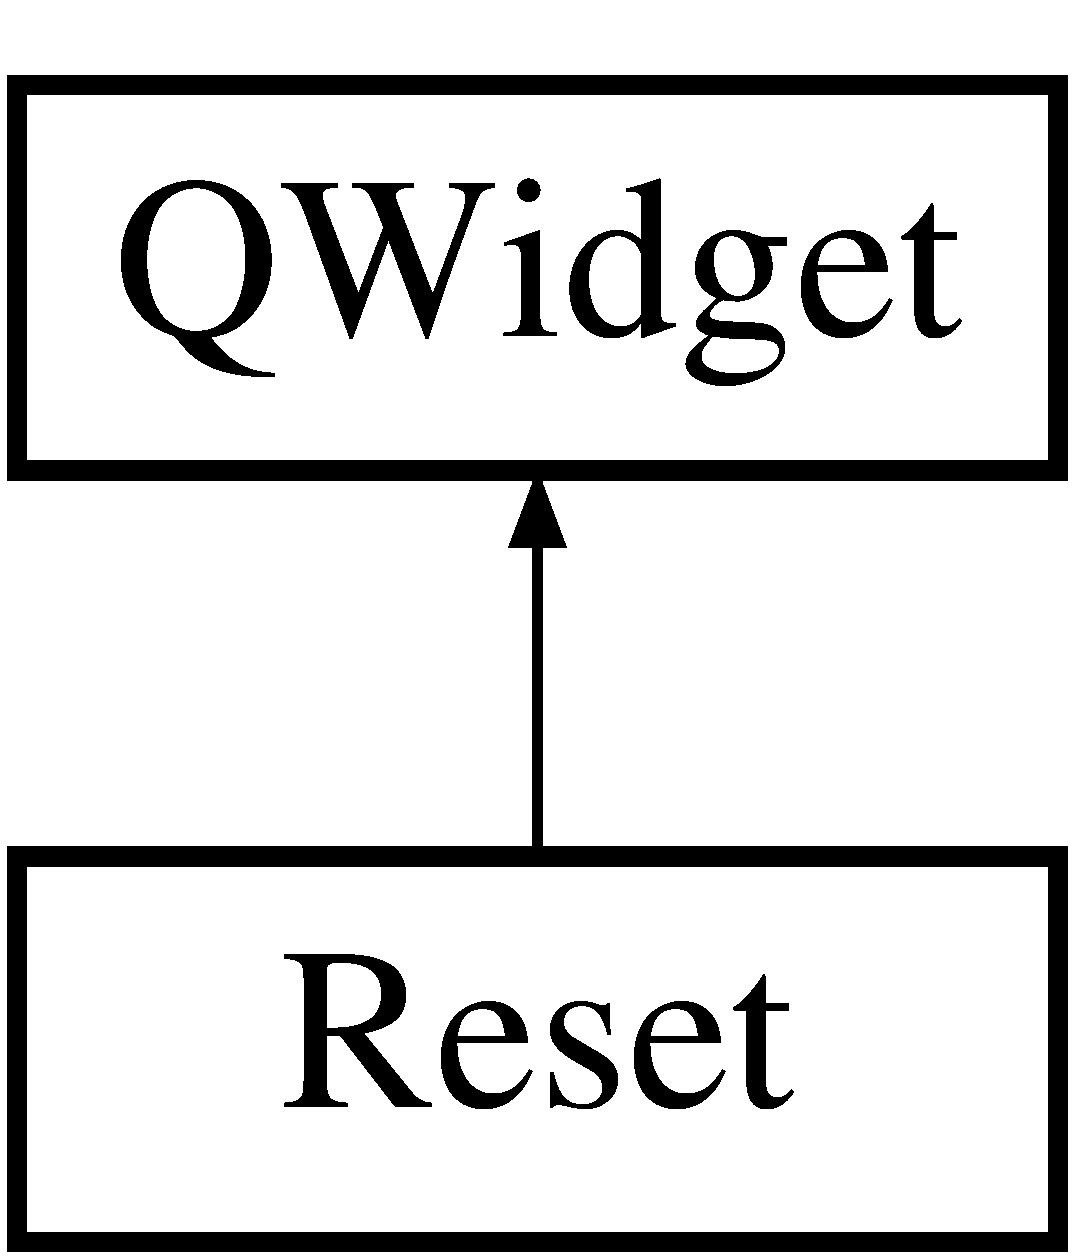
\includegraphics[height=2.000000cm]{class_reset}
\end{center}
\end{figure}
\subsection*{Public Member Functions}
\begin{DoxyCompactItemize}
\item 
\hyperlink{class_reset_a1a9ff0a65a0f9fa43e72174921973c12}{Reset} (Q\+Widget $\ast$parent=0)
\item 
\hyperlink{class_reset_a1d5b1c4b9325560ff386c64e3e6de0f0}{$\sim$\+Reset} ()
\end{DoxyCompactItemize}


\subsection{Detailed Description}
The \hyperlink{class_reset}{Reset} class To confirm reseting of the scores record. 

Definition at line 14 of file reset.\+h.



\subsection{Constructor \& Destructor Documentation}
\hypertarget{class_reset_a1a9ff0a65a0f9fa43e72174921973c12}{}\label{class_reset_a1a9ff0a65a0f9fa43e72174921973c12} 
\index{Reset@{Reset}!Reset@{Reset}}
\index{Reset@{Reset}!Reset@{Reset}}
\subsubsection{\texorpdfstring{Reset()}{Reset()}}
{\footnotesize\ttfamily Reset\+::\+Reset (\begin{DoxyParamCaption}\item[{Q\+Widget $\ast$}]{parent = {\ttfamily 0} }\end{DoxyParamCaption})\hspace{0.3cm}{\ttfamily [explicit]}}



Definition at line 3 of file reset.\+cpp.


\begin{DoxyCode}
4 \{
5 
6 \}
\end{DoxyCode}
\hypertarget{class_reset_a1d5b1c4b9325560ff386c64e3e6de0f0}{}\label{class_reset_a1d5b1c4b9325560ff386c64e3e6de0f0} 
\index{Reset@{Reset}!````~Reset@{$\sim$\+Reset}}
\index{````~Reset@{$\sim$\+Reset}!Reset@{Reset}}
\subsubsection{\texorpdfstring{$\sim$\+Reset()}{~Reset()}}
{\footnotesize\ttfamily Reset\+::$\sim$\+Reset (\begin{DoxyParamCaption}{ }\end{DoxyParamCaption})}



Definition at line 26 of file reset.\+cpp.


\begin{DoxyCode}
26 \{\}
\end{DoxyCode}


The documentation for this class was generated from the following files\+:\begin{DoxyCompactItemize}
\item 
view/\hyperlink{reset_8h}{reset.\+h}\item 
\hyperlink{reset_8cpp}{reset.\+cpp}\end{DoxyCompactItemize}

\hypertarget{classoli_1_1_square}{}\section{oli\+:\+:Square Class Reference}
\label{classoli_1_1_square}\index{oli\+::\+Square@{oli\+::\+Square}}


{\ttfamily \#include $<$square.\+h$>$}

\subsection*{Public Member Functions}
\begin{DoxyCompactItemize}
\item 
\hyperlink{classoli_1_1_square_acc031fb00b69ad310d63985481b60ba6}{Square} ()
\begin{DoxyCompactList}\small\item\em \hyperlink{classoli_1_1_square}{Square} \hyperlink{classoli_1_1_square}{Square}\textquotesingle{}s default constructor. \end{DoxyCompactList}\item 
\hyperlink{classoli_1_1_square_a178d27c0b19d746f052355048847645d}{Square} (\hyperlink{classoli_1_1_position}{Position} position, int nb\+Col)
\begin{DoxyCompactList}\small\item\em \hyperlink{classoli_1_1_square}{Square} square\textquotesingle{}s constructor with parameters. \end{DoxyCompactList}\item 
\hyperlink{classoli_1_1_square_a8d8dbadb3451a21672e4485b75638776}{Square} (\hyperlink{classoli_1_1_position}{Position} position, \hyperlink{namespaceoli_aac44697e43b3ab2ad32fe892ab2276eb}{Color} color)
\begin{DoxyCompactList}\small\item\em \hyperlink{classoli_1_1_square}{Square}. \end{DoxyCompactList}\item 
\hyperlink{classoli_1_1_square_ae3a146c140b1c641391cb0a2f3319719}{$\sim$\+Square} ()
\item 
void \hyperlink{classoli_1_1_square_afd04e5d1eaa2e2f2eaab0be32f2d965f}{set\+Color} (\hyperlink{namespaceoli_aac44697e43b3ab2ad32fe892ab2276eb}{Color} color)
\begin{DoxyCompactList}\small\item\em set\+Color to set the square\textquotesingle{}s color \end{DoxyCompactList}\item 
\hyperlink{namespaceoli_aac44697e43b3ab2ad32fe892ab2276eb}{Color} \hyperlink{classoli_1_1_square_a7709b35684fb5754e53d138bb916880c}{get\+Color} ()
\begin{DoxyCompactList}\small\item\em get\+Color \end{DoxyCompactList}\item 
Q\+Color \hyperlink{classoli_1_1_square_aff2077d95454b98d160c587f13eb10e7}{get\+Q\+Color} ()
\begin{DoxyCompactList}\small\item\em get\+Q\+Color \end{DoxyCompactList}\item 
void \hyperlink{classoli_1_1_square_a1c2449cd8855586cd63d6bde60873ce5}{set\+Captured} ()
\begin{DoxyCompactList}\small\item\em set\+Captured set if the square is captured or not \end{DoxyCompactList}\item 
bool \hyperlink{classoli_1_1_square_aa8ed3521a370df288e9085222660d7ea}{get\+Captured} ()
\begin{DoxyCompactList}\small\item\em get\+Captured \end{DoxyCompactList}\end{DoxyCompactItemize}


\subsection{Detailed Description}


Definition at line 13 of file square.\+h.



\subsection{Constructor \& Destructor Documentation}
\hypertarget{classoli_1_1_square_acc031fb00b69ad310d63985481b60ba6}{}\label{classoli_1_1_square_acc031fb00b69ad310d63985481b60ba6} 
\index{oli\+::\+Square@{oli\+::\+Square}!Square@{Square}}
\index{Square@{Square}!oli\+::\+Square@{oli\+::\+Square}}
\subsubsection{\texorpdfstring{Square()}{Square()}\hspace{0.1cm}{\footnotesize\ttfamily [1/3]}}
{\footnotesize\ttfamily oli\+::\+Square\+::\+Square (\begin{DoxyParamCaption}{ }\end{DoxyParamCaption})}



\hyperlink{classoli_1_1_square}{Square} \hyperlink{classoli_1_1_square}{Square}\textquotesingle{}s default constructor. 



Definition at line 5 of file square.\+cpp.


\begin{DoxyCode}
5               \{
6 
7 \}
\end{DoxyCode}
\hypertarget{classoli_1_1_square_a178d27c0b19d746f052355048847645d}{}\label{classoli_1_1_square_a178d27c0b19d746f052355048847645d} 
\index{oli\+::\+Square@{oli\+::\+Square}!Square@{Square}}
\index{Square@{Square}!oli\+::\+Square@{oli\+::\+Square}}
\subsubsection{\texorpdfstring{Square()}{Square()}\hspace{0.1cm}{\footnotesize\ttfamily [2/3]}}
{\footnotesize\ttfamily oli\+::\+Square\+::\+Square (\begin{DoxyParamCaption}\item[{\hyperlink{classoli_1_1_position}{Position}}]{position,  }\item[{int}]{nb\+Col }\end{DoxyParamCaption})}



\hyperlink{classoli_1_1_square}{Square} square\textquotesingle{}s constructor with parameters. 


\begin{DoxyParams}{Parameters}
{\em position} & the position of the square \\
\hline
{\em nb\+Col} & the square\textquotesingle{}s color \\
\hline
\end{DoxyParams}


Definition at line 8 of file square.\+cpp.


\begin{DoxyCode}
8                                           \{
9     \_position = position;
10         \textcolor{keywordtype}{int} randomNumber = (random(0,nbCol));
11     \_color = \textcolor{keyword}{static\_cast<}\hyperlink{namespaceoli_aac44697e43b3ab2ad32fe892ab2276eb}{Color}\textcolor{keyword}{>}(randomNumber);
12     \_captured = \textcolor{keyword}{false};
13 \}
\end{DoxyCode}
\hypertarget{classoli_1_1_square_a8d8dbadb3451a21672e4485b75638776}{}\label{classoli_1_1_square_a8d8dbadb3451a21672e4485b75638776} 
\index{oli\+::\+Square@{oli\+::\+Square}!Square@{Square}}
\index{Square@{Square}!oli\+::\+Square@{oli\+::\+Square}}
\subsubsection{\texorpdfstring{Square()}{Square()}\hspace{0.1cm}{\footnotesize\ttfamily [3/3]}}
{\footnotesize\ttfamily oli\+::\+Square\+::\+Square (\begin{DoxyParamCaption}\item[{\hyperlink{classoli_1_1_position}{Position}}]{position,  }\item[{\hyperlink{namespaceoli_aac44697e43b3ab2ad32fe892ab2276eb}{Color}}]{color }\end{DoxyParamCaption})}



\hyperlink{classoli_1_1_square}{Square}. 


\begin{DoxyParams}{Parameters}
{\em position} & \\
\hline
{\em color} & \\
\hline
\end{DoxyParams}


Definition at line 15 of file square.\+cpp.


\begin{DoxyCode}
15                                            \{
16     \_position = position;
17     \_color = color;
18 \}
\end{DoxyCode}
\hypertarget{classoli_1_1_square_ae3a146c140b1c641391cb0a2f3319719}{}\label{classoli_1_1_square_ae3a146c140b1c641391cb0a2f3319719} 
\index{oli\+::\+Square@{oli\+::\+Square}!````~Square@{$\sim$\+Square}}
\index{````~Square@{$\sim$\+Square}!oli\+::\+Square@{oli\+::\+Square}}
\subsubsection{\texorpdfstring{$\sim$\+Square()}{~Square()}}
{\footnotesize\ttfamily oli\+::\+Square\+::$\sim$\+Square (\begin{DoxyParamCaption}{ }\end{DoxyParamCaption})}



Definition at line 21 of file square.\+cpp.


\begin{DoxyCode}
21 \{\}
\end{DoxyCode}


\subsection{Member Function Documentation}
\hypertarget{classoli_1_1_square_aa8ed3521a370df288e9085222660d7ea}{}\label{classoli_1_1_square_aa8ed3521a370df288e9085222660d7ea} 
\index{oli\+::\+Square@{oli\+::\+Square}!get\+Captured@{get\+Captured}}
\index{get\+Captured@{get\+Captured}!oli\+::\+Square@{oli\+::\+Square}}
\subsubsection{\texorpdfstring{get\+Captured()}{getCaptured()}}
{\footnotesize\ttfamily bool oli\+::\+Square\+::get\+Captured (\begin{DoxyParamCaption}{ }\end{DoxyParamCaption})}



get\+Captured 

\begin{DoxyReturn}{Returns}
if the square is captured or not 
\end{DoxyReturn}


Definition at line 34 of file square.\+cpp.


\begin{DoxyCode}
34                         \{
35     \textcolor{keywordflow}{return} \_captured;
36 \}
\end{DoxyCode}
\hypertarget{classoli_1_1_square_a7709b35684fb5754e53d138bb916880c}{}\label{classoli_1_1_square_a7709b35684fb5754e53d138bb916880c} 
\index{oli\+::\+Square@{oli\+::\+Square}!get\+Color@{get\+Color}}
\index{get\+Color@{get\+Color}!oli\+::\+Square@{oli\+::\+Square}}
\subsubsection{\texorpdfstring{get\+Color()}{getColor()}}
{\footnotesize\ttfamily \hyperlink{namespaceoli_aac44697e43b3ab2ad32fe892ab2276eb}{Color} oli\+::\+Square\+::get\+Color (\begin{DoxyParamCaption}{ }\end{DoxyParamCaption})}



get\+Color 

\begin{DoxyReturn}{Returns}
the \hyperlink{classoli_1_1_square}{Square}\textquotesingle{}s color 
\end{DoxyReturn}


Definition at line 27 of file square.\+cpp.


\begin{DoxyCode}
27                       \{
28     \textcolor{keywordflow}{return} \_color;
29 \}
\end{DoxyCode}
\hypertarget{classoli_1_1_square_aff2077d95454b98d160c587f13eb10e7}{}\label{classoli_1_1_square_aff2077d95454b98d160c587f13eb10e7} 
\index{oli\+::\+Square@{oli\+::\+Square}!get\+Q\+Color@{get\+Q\+Color}}
\index{get\+Q\+Color@{get\+Q\+Color}!oli\+::\+Square@{oli\+::\+Square}}
\subsubsection{\texorpdfstring{get\+Q\+Color()}{getQColor()}}
{\footnotesize\ttfamily Q\+Color oli\+::\+Square\+::get\+Q\+Color (\begin{DoxyParamCaption}{ }\end{DoxyParamCaption})}



get\+Q\+Color 

\begin{DoxyReturn}{Returns}
the square\textquotesingle{}s Qcolor 
\end{DoxyReturn}
\hypertarget{classoli_1_1_square_a1c2449cd8855586cd63d6bde60873ce5}{}\label{classoli_1_1_square_a1c2449cd8855586cd63d6bde60873ce5} 
\index{oli\+::\+Square@{oli\+::\+Square}!set\+Captured@{set\+Captured}}
\index{set\+Captured@{set\+Captured}!oli\+::\+Square@{oli\+::\+Square}}
\subsubsection{\texorpdfstring{set\+Captured()}{setCaptured()}}
{\footnotesize\ttfamily void oli\+::\+Square\+::set\+Captured (\begin{DoxyParamCaption}{ }\end{DoxyParamCaption})}



set\+Captured set if the square is captured or not 



Definition at line 31 of file square.\+cpp.


\begin{DoxyCode}
31                         \{
32     \_captured = \textcolor{keyword}{true};
33 \}
\end{DoxyCode}
\hypertarget{classoli_1_1_square_afd04e5d1eaa2e2f2eaab0be32f2d965f}{}\label{classoli_1_1_square_afd04e5d1eaa2e2f2eaab0be32f2d965f} 
\index{oli\+::\+Square@{oli\+::\+Square}!set\+Color@{set\+Color}}
\index{set\+Color@{set\+Color}!oli\+::\+Square@{oli\+::\+Square}}
\subsubsection{\texorpdfstring{set\+Color()}{setColor()}}
{\footnotesize\ttfamily void oli\+::\+Square\+::set\+Color (\begin{DoxyParamCaption}\item[{\hyperlink{namespaceoli_aac44697e43b3ab2ad32fe892ab2276eb}{Color}}]{color }\end{DoxyParamCaption})}



set\+Color to set the square\textquotesingle{}s color 


\begin{DoxyParams}{Parameters}
{\em color} & the color to set \\
\hline
\end{DoxyParams}


Definition at line 23 of file square.\+cpp.


\begin{DoxyCode}
23                                 \{
24     \_color = color;
25 \}
\end{DoxyCode}


The documentation for this class was generated from the following files\+:\begin{DoxyCompactItemize}
\item 
model/\hyperlink{square_8h}{square.\+h}\item 
model/\hyperlink{square_8cpp}{square.\+cpp}\end{DoxyCompactItemize}

\hypertarget{classoli_1_1_view_board}{}\section{oli\+:\+:View\+Board Class Reference}
\label{classoli_1_1_view_board}\index{oli\+::\+View\+Board@{oli\+::\+View\+Board}}


The \hyperlink{classoli_1_1_view_board}{View\+Board} class the class that create and refresh the game\textquotesingle{}s board view.  




{\ttfamily \#include $<$viewboard.\+h$>$}

Inheritance diagram for oli\+:\+:View\+Board\+:\begin{figure}[H]
\begin{center}
\leavevmode
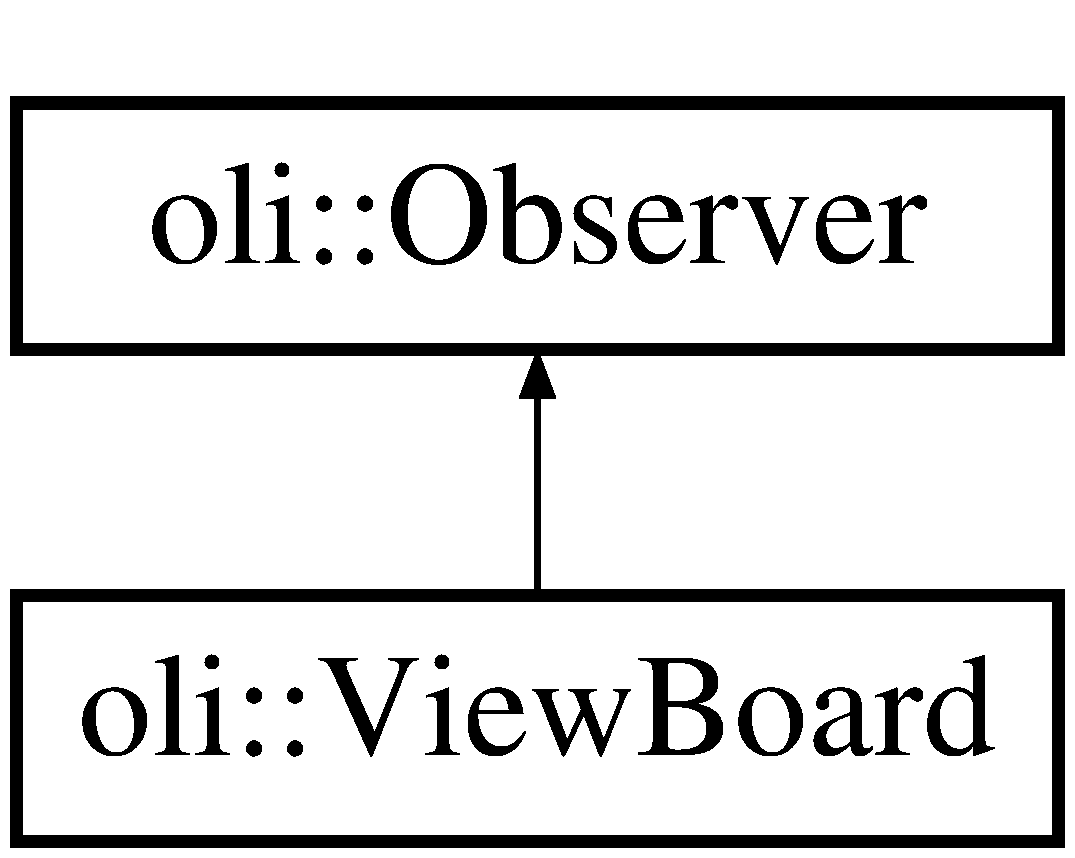
\includegraphics[height=2.000000cm]{classoli_1_1_view_board}
\end{center}
\end{figure}
\subsection*{Signals}
\begin{DoxyCompactItemize}
\item 
void \hyperlink{classoli_1_1_view_board_a6490954a9baf4e72e899ba10a4f414b7}{test} ()
\end{DoxyCompactItemize}
\subsection*{Public Member Functions}
\begin{DoxyCompactItemize}
\item 
\hyperlink{classoli_1_1_view_board_a36385a4f3f367326ad864c64e6dff4bc}{View\+Board} ()
\item 
\hyperlink{classoli_1_1_view_board_a0d4a844b1b5450ab623a747b7ced2e59}{View\+Board} (Q\+Widget \&fenetre, \hyperlink{classoli_1_1_floodgame}{Floodgame} $\ast$game, int nb\+Col)
\item 
void \hyperlink{classoli_1_1_view_board_a0f9e3b18dfb6f2224bef1b73ce8b3929}{set\+Display} ()
\item 
void \hyperlink{classoli_1_1_view_board_a487ea5886ec5de0422fc6e060aa7045b}{Update} ()
\end{DoxyCompactItemize}
\subsection*{Additional Inherited Members}


\subsection{Detailed Description}
The \hyperlink{classoli_1_1_view_board}{View\+Board} class the class that create and refresh the game\textquotesingle{}s board view. 

Definition at line 19 of file viewboard.\+h.



\subsection{Constructor \& Destructor Documentation}
\hypertarget{classoli_1_1_view_board_a36385a4f3f367326ad864c64e6dff4bc}{}\label{classoli_1_1_view_board_a36385a4f3f367326ad864c64e6dff4bc} 
\index{oli\+::\+View\+Board@{oli\+::\+View\+Board}!View\+Board@{View\+Board}}
\index{View\+Board@{View\+Board}!oli\+::\+View\+Board@{oli\+::\+View\+Board}}
\subsubsection{\texorpdfstring{View\+Board()}{ViewBoard()}\hspace{0.1cm}{\footnotesize\ttfamily [1/2]}}
{\footnotesize\ttfamily oli\+::\+View\+Board\+::\+View\+Board (\begin{DoxyParamCaption}{ }\end{DoxyParamCaption})}



Definition at line 5 of file viewboard.\+cpp.


\begin{DoxyCode}
5 \{\}
\end{DoxyCode}
\hypertarget{classoli_1_1_view_board_a0d4a844b1b5450ab623a747b7ced2e59}{}\label{classoli_1_1_view_board_a0d4a844b1b5450ab623a747b7ced2e59} 
\index{oli\+::\+View\+Board@{oli\+::\+View\+Board}!View\+Board@{View\+Board}}
\index{View\+Board@{View\+Board}!oli\+::\+View\+Board@{oli\+::\+View\+Board}}
\subsubsection{\texorpdfstring{View\+Board()}{ViewBoard()}\hspace{0.1cm}{\footnotesize\ttfamily [2/2]}}
{\footnotesize\ttfamily oli\+::\+View\+Board\+::\+View\+Board (\begin{DoxyParamCaption}\item[{Q\+Widget \&}]{fenetre,  }\item[{\hyperlink{classoli_1_1_floodgame}{Floodgame} $\ast$}]{game,  }\item[{int}]{nb\+Col }\end{DoxyParamCaption})}



Definition at line 7 of file viewboard.\+cpp.


\begin{DoxyCode}
7                                                                 \{
8 
9     \_game = game;
10     \_ql = \textcolor{keyword}{new} QLabel(&fenetre);
11     \_ql->setFixedHeight(525);
12 
13     \_gameOver = \textcolor{keyword}{new} QLabel(&fenetre);
14     \_gameOver->setFixedHeight(525);
15     \_gameOver->setFixedWidth(720);
16     \_gameOver->setAlignment(Qt::AlignCenter);
17 
18     \_buttonWidget = \textcolor{keyword}{new} ButtonWidget(nbCol,&fenetre);
19     \_vBox = \textcolor{keyword}{new} QVBoxLayout();
20     \_hboxBoutons = \textcolor{keyword}{new} QHBoxLayout;
21     \_record = \textcolor{keyword}{new} QLabel(&fenetre);
22     \_nbClickLabel = \textcolor{keyword}{new} QLabel(&fenetre);
23 
24     QPushButton *restart = \textcolor{keyword}{new} QPushButton(\textcolor{stringliteral}{"Restart"});
25     QPushButton *quit = \textcolor{keyword}{new} QPushButton(\textcolor{stringliteral}{"Quit"});
26 
27     QObject::connect(quit,SIGNAL(clicked()),&fenetre,SLOT(reemit()));
28     QObject::connect(restart,SIGNAL(clicked()),&fenetre,SLOT(restart()));
29 
30     quit->setSizePolicy(QSizePolicy::Fixed,QSizePolicy::Fixed);
31     restart->setSizePolicy(QSizePolicy::Fixed,QSizePolicy::Fixed);
32 
33     \_hboxBoutons->addWidget(restart);
34     \_hboxBoutons->addWidget(quit);
35     \_hboxBoutons->setAlignment(restart,Qt::AlignRight);
36     \_hboxBoutons->setAlignment(quit,Qt::AlignLeft);
37 
38     fenetre.setLayout(\_vBox);
39     \hyperlink{classoli_1_1_view_board_a0f9e3b18dfb6f2224bef1b73ce8b3929}{setDisplay}();
40 
41     \_vBox->addWidget(\_ql);
42     \_vBox->addWidget(\_record);
43     \_vBox->addWidget(\_nbClickLabel);
44     \_vBox->addWidget(\_buttonWidget);
45     \_vBox->setAlignment(\_buttonWidget,Qt::AlignHCenter);
46 
47     \_vBox->addLayout(\_hboxBoutons);
48 
49 \}
\end{DoxyCode}


\subsection{Member Function Documentation}
\hypertarget{classoli_1_1_view_board_a0f9e3b18dfb6f2224bef1b73ce8b3929}{}\label{classoli_1_1_view_board_a0f9e3b18dfb6f2224bef1b73ce8b3929} 
\index{oli\+::\+View\+Board@{oli\+::\+View\+Board}!set\+Display@{set\+Display}}
\index{set\+Display@{set\+Display}!oli\+::\+View\+Board@{oli\+::\+View\+Board}}
\subsubsection{\texorpdfstring{set\+Display()}{setDisplay()}}
{\footnotesize\ttfamily void oli\+::\+View\+Board\+::set\+Display (\begin{DoxyParamCaption}{ }\end{DoxyParamCaption})}



Definition at line 51 of file viewboard.\+cpp.


\begin{DoxyCode}
51                           \{
52 
53     \textcolor{keywordflow}{if}((\_valueRecord =\_game->\hyperlink{classoli_1_1_floodgame_af0084c4fecf2b51da6aed1f73de05e9e}{getRecord}())==0)\{
54         \_record->setText(\textcolor{stringliteral}{""});
55     \}\textcolor{keywordflow}{else}\{
56         \_record->setText(\textcolor{stringliteral}{"Record: "}+QVariant(\_valueRecord).toString()+\textcolor{stringliteral}{" clicks"});
57         \_record->setAlignment(Qt::AlignCenter);
58         \_record->setStyleSheet(\textcolor{stringliteral}{"QLabel \{ background-color : transparent; color : orange; \}"});
59     \}
60 
61     \_nbClickLabel->setText(\textcolor{stringliteral}{"Clicked "}+QVariant(\_game->\hyperlink{classoli_1_1_floodgame_aae08dd4e048b1521797c44a68d08f250}{getNbClick}()).toString() +\textcolor{stringliteral}{" times"});
62     \_nbClickLabel->setAlignment(Qt::AlignCenter);
63     \_nbClickLabel->setStyleSheet(\textcolor{stringliteral}{"QLabel \{ background-color : transparent; color : white; \}"});
64 
65     \_width = \_game->\hyperlink{classoli_1_1_floodgame_a4775f2321f034778d4de93a888d2283b}{getBoard}().\hyperlink{classoli_1_1_board_a228d72d2aa8a9df2f545ecef14e72a0d}{getWidth}();
66     \_height = \_game->\hyperlink{classoli_1_1_floodgame_a4775f2321f034778d4de93a888d2283b}{getBoard}().\hyperlink{classoli_1_1_board_a17dce7dacfe888f52dfad0468ae51ace}{getHeight}();
67 
68     \textcolor{keywordtype}{int} brolWidth = \_width;
69     \textcolor{keywordtype}{int} brolHeight = \_height;
70     \textcolor{keywordtype}{int} block\_width = 500 / [brolWidth, brolHeight]()\{
71         \textcolor{keywordtype}{int} x;
72         (brolWidth > brolHeight) ? x = brolWidth : x = brolHeight;
73         \textcolor{keywordflow}{return} x;
74     \}();
75     QPixmap \_pixmap;
76     \textcolor{keywordflow}{if}(!\_game->\hyperlink{classoli_1_1_floodgame_adfcb41900bae06b64a8d4d77164b67d5}{isGameOver}())\{
77         \_pixmap= QPixmap(\_width*block\_width+1,\_height*block\_width+1);
78     \}
79     \textcolor{keywordflow}{else} \_pixmap = QPixmap(490,490);
80     \_pixmap.fill(QColor(\textcolor{stringliteral}{"blue"}));
81     \textcolor{keywordflow}{if}(!\_game->\hyperlink{classoli_1_1_floodgame_adfcb41900bae06b64a8d4d77164b67d5}{isGameOver}())\{
82         \textcolor{keywordflow}{for}(\textcolor{keywordtype}{int} i = 0; i < \_height; i++)\{
83             \textcolor{keywordflow}{for} (\textcolor{keywordtype}{int} j = 0; j < \_width; j++)\{
84                 QPainter painter(&\_pixmap);
85                 painter.setPen(QColor(81,81,81,255));
86                 painter.setBrush(\hyperlink{classoli_1_1_color_convert_a4c41280d24ad2cba4b2a46fbb03f2356}{ColorConvert::getQColor}(\_game->
      \hyperlink{classoli_1_1_floodgame_a4775f2321f034778d4de93a888d2283b}{getBoard}().\hyperlink{classoli_1_1_board_a5c1ce624776b1169ee16d8d815e9a453}{getSquare}(i,j).\hyperlink{classoli_1_1_square_a7709b35684fb5754e53d138bb916880c}{getColor}()));
87                 QRect myQRect=(QRect(j*block\_width,i*block\_width,block\_width,block\_width));
88                 painter.drawRect(myQRect);
89             \}
90         \}
91     \}
92     \textcolor{keywordflow}{if}(\_game->\hyperlink{classoli_1_1_floodgame_adfcb41900bae06b64a8d4d77164b67d5}{isGameOver}() && \_game->\hyperlink{classoli_1_1_floodgame_a35b5e1c7f39c73d7d46b8c71156fbfbc}{isNewRecord}())\{
93         \_gameOver->setPixmap(QPixmap(\textcolor{stringliteral}{":/images/highScore.png"}).scaled(QSize(300,300),  Qt::KeepAspectRatio)
      );
94     \}
95     \textcolor{keywordflow}{else} \textcolor{keywordflow}{if}(\_game->\hyperlink{classoli_1_1_floodgame_adfcb41900bae06b64a8d4d77164b67d5}{isGameOver}())\{
96         \_gameOver->setPixmap(QPixmap(\textcolor{stringliteral}{":/images/gameOver2.png"}).scaled(QSize(300,300),  Qt::KeepAspectRatio)
      );
97     \}
98     \textcolor{keywordflow}{else} \_gameOver->setPixmap(QPixmap(\textcolor{stringliteral}{""}));
99     \_ql->setAlignment(Qt::AlignCenter);
100 
101     \_ql->setPixmap(\_pixmap);
102 
103 \}
\end{DoxyCode}
\hypertarget{classoli_1_1_view_board_a6490954a9baf4e72e899ba10a4f414b7}{}\label{classoli_1_1_view_board_a6490954a9baf4e72e899ba10a4f414b7} 
\index{oli\+::\+View\+Board@{oli\+::\+View\+Board}!test@{test}}
\index{test@{test}!oli\+::\+View\+Board@{oli\+::\+View\+Board}}
\subsubsection{\texorpdfstring{test}{test}}
{\footnotesize\ttfamily void oli\+::\+View\+Board\+::test (\begin{DoxyParamCaption}{ }\end{DoxyParamCaption})\hspace{0.3cm}{\ttfamily [signal]}}

\hypertarget{classoli_1_1_view_board_a487ea5886ec5de0422fc6e060aa7045b}{}\label{classoli_1_1_view_board_a487ea5886ec5de0422fc6e060aa7045b} 
\index{oli\+::\+View\+Board@{oli\+::\+View\+Board}!Update@{Update}}
\index{Update@{Update}!oli\+::\+View\+Board@{oli\+::\+View\+Board}}
\subsubsection{\texorpdfstring{Update()}{Update()}}
{\footnotesize\ttfamily void oli\+::\+View\+Board\+::\+Update (\begin{DoxyParamCaption}{ }\end{DoxyParamCaption})\hspace{0.3cm}{\ttfamily [virtual]}}



Implements \hyperlink{classoli_1_1_observer_a81154a42166f88a6e341909438a07b75}{oli\+::\+Observer}.



Definition at line 105 of file viewboard.\+cpp.


\begin{DoxyCode}
105                       \{
106     \hyperlink{classoli_1_1_view_board_a0f9e3b18dfb6f2224bef1b73ce8b3929}{setDisplay}();
107 \}
\end{DoxyCode}


The documentation for this class was generated from the following files\+:\begin{DoxyCompactItemize}
\item 
view/\hyperlink{viewboard_8h}{viewboard.\+h}\item 
view/\hyperlink{viewboard_8cpp}{viewboard.\+cpp}\end{DoxyCompactItemize}

\hypertarget{class_widget_game}{}\section{Widget\+Game Class Reference}
\label{class_widget_game}\index{Widget\+Game@{Widget\+Game}}


The \hyperlink{class_widget_game}{Widget\+Game} class the widget containing the game\textquotesingle{}s view.  




{\ttfamily \#include $<$widget\+Game.\+h$>$}

Inheritance diagram for Widget\+Game\+:\begin{figure}[H]
\begin{center}
\leavevmode
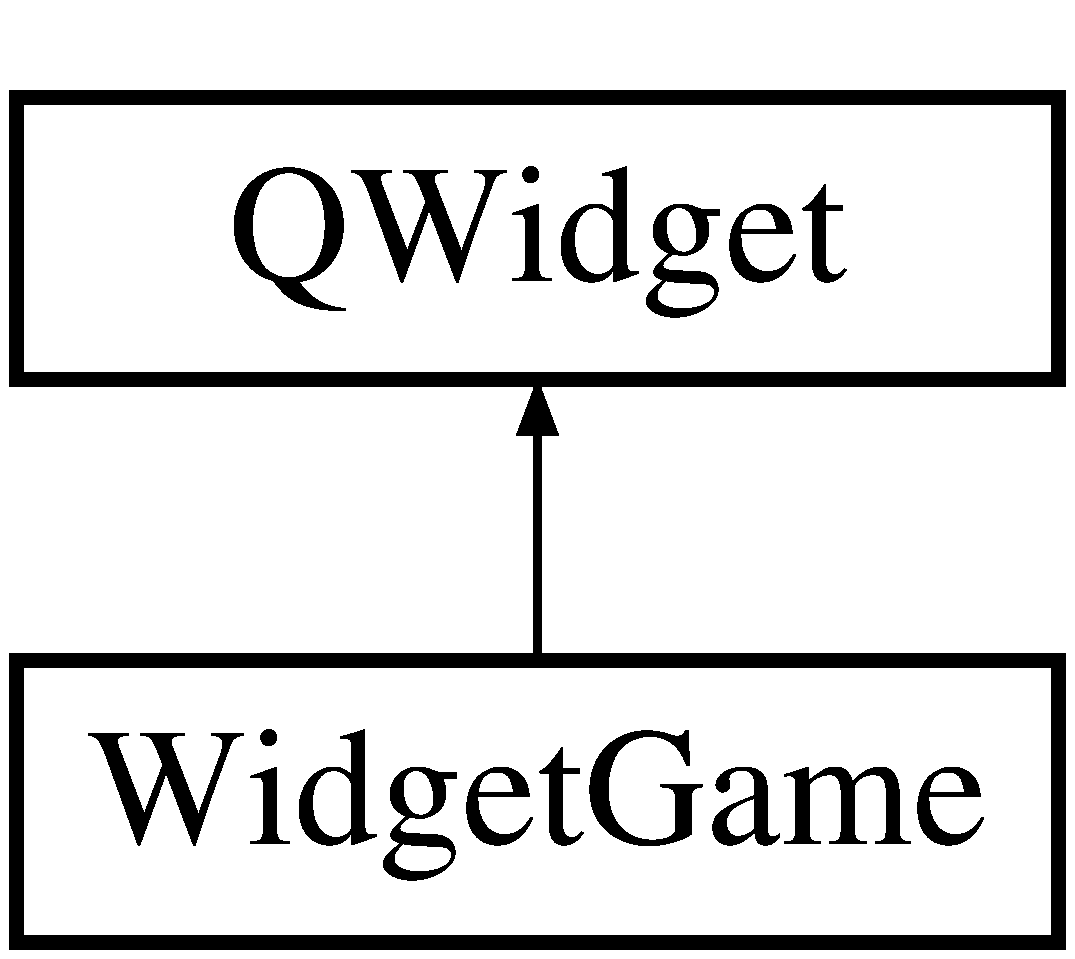
\includegraphics[height=2.000000cm]{class_widget_game}
\end{center}
\end{figure}
\subsection*{Signals}
\begin{DoxyCompactItemize}
\item 
void \hyperlink{class_widget_game_a39c76aac5eff9242d2253017c1209027}{reemit\+Main} ()
\end{DoxyCompactItemize}
\subsection*{Public Member Functions}
\begin{DoxyCompactItemize}
\item 
\hyperlink{class_widget_game_a0c95303c9fc87b64d5fd3cd4f4fb5844}{Widget\+Game} (int height, int width, int nb\+Col, Q\+Widget $\ast$parent=0)
\item 
\hyperlink{class_widget_game_a5164870bf08c80da133fc075298347cc}{$\sim$\+Widget\+Game} ()
\end{DoxyCompactItemize}


\subsection{Detailed Description}
The \hyperlink{class_widget_game}{Widget\+Game} class the widget containing the game\textquotesingle{}s view. 

Definition at line 16 of file widget\+Game.\+h.



\subsection{Constructor \& Destructor Documentation}
\hypertarget{class_widget_game_a0c95303c9fc87b64d5fd3cd4f4fb5844}{}\label{class_widget_game_a0c95303c9fc87b64d5fd3cd4f4fb5844} 
\index{Widget\+Game@{Widget\+Game}!Widget\+Game@{Widget\+Game}}
\index{Widget\+Game@{Widget\+Game}!Widget\+Game@{Widget\+Game}}
\subsubsection{\texorpdfstring{Widget\+Game()}{WidgetGame()}}
{\footnotesize\ttfamily Widget\+Game\+::\+Widget\+Game (\begin{DoxyParamCaption}\item[{int}]{height,  }\item[{int}]{width,  }\item[{int}]{nb\+Col,  }\item[{Q\+Widget $\ast$}]{parent = {\ttfamily 0} }\end{DoxyParamCaption})\hspace{0.3cm}{\ttfamily [explicit]}}



Definition at line 4 of file widget\+Game.\+cpp.


\begin{DoxyCode}
4                                                                      :
5     QWidget(parent)
6 \{
7     \_game = \textcolor{keyword}{new} \hyperlink{classoli_1_1_floodgame}{Floodgame}(height,width,nbCol);
8     \_viewboard = \hyperlink{classoli_1_1_view_board}{ViewBoard}(*\textcolor{keyword}{this},\_game,nbCol);
9     \_game->\hyperlink{classoli_1_1_observable_af746a8f49e2b08bc93767281dd813532}{AddObs}(&\_viewboard);
10 
11     connect(\textcolor{keyword}{this},SIGNAL(\hyperlink{class_widget_game_a39c76aac5eff9242d2253017c1209027}{reemitMain}()),parent,SLOT(cancel()));
12 \}
\end{DoxyCode}
\hypertarget{class_widget_game_a5164870bf08c80da133fc075298347cc}{}\label{class_widget_game_a5164870bf08c80da133fc075298347cc} 
\index{Widget\+Game@{Widget\+Game}!````~Widget\+Game@{$\sim$\+Widget\+Game}}
\index{````~Widget\+Game@{$\sim$\+Widget\+Game}!Widget\+Game@{Widget\+Game}}
\subsubsection{\texorpdfstring{$\sim$\+Widget\+Game()}{~WidgetGame()}}
{\footnotesize\ttfamily Widget\+Game\+::$\sim$\+Widget\+Game (\begin{DoxyParamCaption}{ }\end{DoxyParamCaption})}



Definition at line 14 of file widget\+Game.\+cpp.


\begin{DoxyCode}
14 \{\}
\end{DoxyCode}


\subsection{Member Function Documentation}
\hypertarget{class_widget_game_a39c76aac5eff9242d2253017c1209027}{}\label{class_widget_game_a39c76aac5eff9242d2253017c1209027} 
\index{Widget\+Game@{Widget\+Game}!reemit\+Main@{reemit\+Main}}
\index{reemit\+Main@{reemit\+Main}!Widget\+Game@{Widget\+Game}}
\subsubsection{\texorpdfstring{reemit\+Main}{reemitMain}}
{\footnotesize\ttfamily void Widget\+Game\+::reemit\+Main (\begin{DoxyParamCaption}{ }\end{DoxyParamCaption})\hspace{0.3cm}{\ttfamily [signal]}}



The documentation for this class was generated from the following files\+:\begin{DoxyCompactItemize}
\item 
view/\hyperlink{widget_game_8h}{widget\+Game.\+h}\item 
view/\hyperlink{widget_game_8cpp}{widget\+Game.\+cpp}\end{DoxyCompactItemize}

\chapter{File Documentation}
\hypertarget{main_8cpp}{}\section{main.\+cpp File Reference}
\label{main_8cpp}\index{main.\+cpp@{main.\+cpp}}
{\ttfamily \#include \char`\"{}view/mainwindow.\+h\char`\"{}}\newline
{\ttfamily \#include $<$Q\+Application$>$}\newline
{\ttfamily \#include $<$Q\+Message\+Box$>$}\newline
\subsection*{Functions}
\begin{DoxyCompactItemize}
\item 
int \hyperlink{main_8cpp_a0ddf1224851353fc92bfbff6f499fa97}{main} (int argc, char $\ast$argv\mbox{[}$\,$\mbox{]})
\end{DoxyCompactItemize}


\subsection{Function Documentation}
\hypertarget{main_8cpp_a0ddf1224851353fc92bfbff6f499fa97}{}\label{main_8cpp_a0ddf1224851353fc92bfbff6f499fa97} 
\index{main.\+cpp@{main.\+cpp}!main@{main}}
\index{main@{main}!main.\+cpp@{main.\+cpp}}
\subsubsection{\texorpdfstring{main()}{main()}}
{\footnotesize\ttfamily int main (\begin{DoxyParamCaption}\item[{int}]{argc,  }\item[{char $\ast$}]{argv\mbox{[}$\,$\mbox{]} }\end{DoxyParamCaption})}



Definition at line 6 of file main.\+cpp.


\begin{DoxyCode}
7 \{
8     QApplication a(argc, argv);
9     \hyperlink{class_main_window}{MainWindow} w;
10     w.setFixedSize(720,660);
11     w.setWindowTitle(\textcolor{stringliteral}{"Flood it by Olivier.C"});
12     w.show();
13 
14     \textcolor{keywordflow}{return} a.exec();
15 \}
\end{DoxyCode}

\hypertarget{board_8cpp}{}\section{model/board.cpp File Reference}
\label{board_8cpp}\index{model/board.\+cpp@{model/board.\+cpp}}
{\ttfamily \#include \char`\"{}board.\+h\char`\"{}}\newline
{\ttfamily \#include \char`\"{}square.\+h\char`\"{}}\newline
\subsection*{Namespaces}
\begin{DoxyCompactItemize}
\item 
 \hyperlink{namespaceoli}{oli}
\end{DoxyCompactItemize}

\hypertarget{board_8h}{}\section{model/board.h File Reference}
\label{board_8h}\index{model/board.\+h@{model/board.\+h}}
{\ttfamily \#include $<$vector$>$}\newline
{\ttfamily \#include \char`\"{}square.\+h\char`\"{}}\newline
{\ttfamily \#include \char`\"{}floodexception.\+h\char`\"{}}\newline
\subsection*{Classes}
\begin{DoxyCompactItemize}
\item 
class \hyperlink{classoli_1_1_board}{oli\+::\+Board}
\begin{DoxyCompactList}\small\item\em The \hyperlink{classoli_1_1_board}{Board} class. \end{DoxyCompactList}\end{DoxyCompactItemize}
\subsection*{Namespaces}
\begin{DoxyCompactItemize}
\item 
 \hyperlink{namespaceoli}{oli}
\end{DoxyCompactItemize}

\hypertarget{color_8h}{}\section{model/color.h File Reference}
\label{color_8h}\index{model/color.\+h@{model/color.\+h}}
\subsection*{Namespaces}
\begin{DoxyCompactItemize}
\item 
 \hyperlink{namespaceoli}{oli}
\end{DoxyCompactItemize}
\subsection*{Enumerations}
\begin{DoxyCompactItemize}
\item 
enum \hyperlink{namespaceoli_aac44697e43b3ab2ad32fe892ab2276eb}{oli\+::\+Color} \{ \newline
\hyperlink{namespaceoli_aac44697e43b3ab2ad32fe892ab2276ebaa2d9547b5d3dd9f05984475f7c926da0}{oli\+::\+Color\+::\+R\+ED}, 
\hyperlink{namespaceoli_aac44697e43b3ab2ad32fe892ab2276eba9de0e5dd94e861317e74964bed179fa0}{oli\+::\+Color\+::\+G\+R\+E\+EN}, 
\hyperlink{namespaceoli_aac44697e43b3ab2ad32fe892ab2276eba8a568e5f41b7e4da88fe5c4a00aad34e}{oli\+::\+Color\+::\+Y\+E\+L\+L\+OW}, 
\hyperlink{namespaceoli_aac44697e43b3ab2ad32fe892ab2276eba1b3e1ee9bff86431dea6b181365ba65f}{oli\+::\+Color\+::\+B\+L\+UE}, 
\newline
\hyperlink{namespaceoli_aac44697e43b3ab2ad32fe892ab2276ebaec9c138095a352a9b7ef9ca5363b14d9}{oli\+::\+Color\+::\+P\+U\+R\+P\+LE}, 
\hyperlink{namespaceoli_aac44697e43b3ab2ad32fe892ab2276eba90c86d1e3da733aaf155dcc24f2a235b}{oli\+::\+Color\+::\+D\+E\+E\+P\+P\+I\+NK}, 
\hyperlink{namespaceoli_aac44697e43b3ab2ad32fe892ab2276eba344dd8cd533280795b9db82ef0c92749}{oli\+::\+Color\+::\+C\+Y\+AN}, 
\hyperlink{namespaceoli_aac44697e43b3ab2ad32fe892ab2276eba5b6490317b6f7270bc3ab5ffd07c1f52}{oli\+::\+Color\+::\+O\+R\+A\+N\+GE}, 
\newline
\hyperlink{namespaceoli_aac44697e43b3ab2ad32fe892ab2276eba3c551f0d1a06b4f852d1832daed357bf}{oli\+::\+Color\+::\+G\+R\+EY}
 \}\begin{DoxyCompactList}\small\item\em The Color enum This enumeration is used to set a color to a square. \end{DoxyCompactList}
\end{DoxyCompactItemize}

\hypertarget{floodexception_8h}{}\section{model/floodexception.h File Reference}
\label{floodexception_8h}\index{model/floodexception.\+h@{model/floodexception.\+h}}
{\ttfamily \#include $<$iostream$>$}\newline
{\ttfamily \#include $<$sstream$>$}\newline
{\ttfamily \#include $<$exception$>$}\newline
\subsection*{Classes}
\begin{DoxyCompactItemize}
\item 
class \hyperlink{classoli_1_1_flood_exception}{oli\+::\+Flood\+Exception}
\begin{DoxyCompactList}\small\item\em The \hyperlink{classoli_1_1_flood_exception}{Flood\+Exception} class This is the exception class used for the game . \end{DoxyCompactList}\end{DoxyCompactItemize}
\subsection*{Namespaces}
\begin{DoxyCompactItemize}
\item 
 \hyperlink{namespaceoli}{oli}
\end{DoxyCompactItemize}

\hypertarget{floodgame_8cpp}{}\section{model/floodgame.cpp File Reference}
\label{floodgame_8cpp}\index{model/floodgame.\+cpp@{model/floodgame.\+cpp}}
{\ttfamily \#include \char`\"{}floodgame.\+h\char`\"{}}\newline
\subsection*{Namespaces}
\begin{DoxyCompactItemize}
\item 
 \hyperlink{namespaceoli}{oli}
\end{DoxyCompactItemize}

\hypertarget{floodgame_8h}{}\section{model/floodgame.h File Reference}
\label{floodgame_8h}\index{model/floodgame.\+h@{model/floodgame.\+h}}
{\ttfamily \#include $<$list$>$}\newline
{\ttfamily \#include $<$model/color.\+h$>$}\newline
{\ttfamily \#include $<$Q\+Json\+Object$>$}\newline
{\ttfamily \#include $<$Q\+Json\+Document$>$}\newline
{\ttfamily \#include $<$iostream$>$}\newline
{\ttfamily \#include $<$Q\+File$>$}\newline
{\ttfamily \#include \char`\"{}High\+Score.\+h\char`\"{}}\newline
{\ttfamily \#include \char`\"{}model/board.\+h\char`\"{}}\newline
{\ttfamily \#include \char`\"{}observer/observable.\+h\char`\"{}}\newline
\subsection*{Classes}
\begin{DoxyCompactItemize}
\item 
class \hyperlink{classoli_1_1_floodgame}{oli\+::\+Floodgame}
\end{DoxyCompactItemize}
\subsection*{Namespaces}
\begin{DoxyCompactItemize}
\item 
 \hyperlink{namespaceoli}{oli}
\end{DoxyCompactItemize}

\hypertarget{_high_score_8cpp}{}\section{model/\+High\+Score.cpp File Reference}
\label{_high_score_8cpp}\index{model/\+High\+Score.\+cpp@{model/\+High\+Score.\+cpp}}
{\ttfamily \#include \char`\"{}High\+Score.\+h\char`\"{}}\newline
\subsection*{Namespaces}
\begin{DoxyCompactItemize}
\item 
 \hyperlink{namespaceoli}{oli}
\end{DoxyCompactItemize}

\hypertarget{_high_score_8h}{}\section{model/\+High\+Score.h File Reference}
\label{_high_score_8h}\index{model/\+High\+Score.\+h@{model/\+High\+Score.\+h}}
{\ttfamily \#include $<$Q\+Json\+Object$>$}\newline
{\ttfamily \#include $<$sstream$>$}\newline
\subsection*{Classes}
\begin{DoxyCompactItemize}
\item 
class \hyperlink{classoli_1_1_high_score}{oli\+::\+High\+Score}
\begin{DoxyCompactList}\small\item\em The \hyperlink{classoli_1_1_high_score}{High\+Score} class Used to compare old results and the new score according to the weight, the height and the number of colors function. \end{DoxyCompactList}\end{DoxyCompactItemize}
\subsection*{Namespaces}
\begin{DoxyCompactItemize}
\item 
 \hyperlink{namespaceoli}{oli}
\end{DoxyCompactItemize}

\hypertarget{position_8cpp}{}\section{model/position.cpp File Reference}
\label{position_8cpp}\index{model/position.\+cpp@{model/position.\+cpp}}
{\ttfamily \#include \char`\"{}position.\+h\char`\"{}}\newline
\subsection*{Namespaces}
\begin{DoxyCompactItemize}
\item 
 \hyperlink{namespaceoli}{oli}
\end{DoxyCompactItemize}

\hypertarget{position_8h}{}\section{model/position.h File Reference}
\label{position_8h}\index{model/position.\+h@{model/position.\+h}}
\subsection*{Classes}
\begin{DoxyCompactItemize}
\item 
class \hyperlink{classoli_1_1_position}{oli\+::\+Position}
\begin{DoxyCompactList}\small\item\em The \hyperlink{classoli_1_1_position}{Position} class. \end{DoxyCompactList}\end{DoxyCompactItemize}
\subsection*{Namespaces}
\begin{DoxyCompactItemize}
\item 
 \hyperlink{namespaceoli}{oli}
\end{DoxyCompactItemize}

\hypertarget{square_8cpp}{}\section{model/square.cpp File Reference}
\label{square_8cpp}\index{model/square.\+cpp@{model/square.\+cpp}}
{\ttfamily \#include \char`\"{}square.\+h\char`\"{}}\newline
\subsection*{Namespaces}
\begin{DoxyCompactItemize}
\item 
 \hyperlink{namespaceoli}{oli}
\end{DoxyCompactItemize}

\hypertarget{square_8h}{}\section{model/square.h File Reference}
\label{square_8h}\index{model/square.\+h@{model/square.\+h}}
{\ttfamily \#include $<$Q\+Color$>$}\newline
{\ttfamily \#include $<$random$>$}\newline
{\ttfamily \#include $<$iostream$>$}\newline
{\ttfamily \#include $<$time.\+h$>$}\newline
{\ttfamily \#include \char`\"{}color.\+h\char`\"{}}\newline
{\ttfamily \#include \char`\"{}position.\+h\char`\"{}}\newline
\subsection*{Classes}
\begin{DoxyCompactItemize}
\item 
class \hyperlink{classoli_1_1_square}{oli\+::\+Square}
\end{DoxyCompactItemize}
\subsection*{Namespaces}
\begin{DoxyCompactItemize}
\item 
 \hyperlink{namespaceoli}{oli}
\end{DoxyCompactItemize}

\hypertarget{observable_8cpp}{}\section{observer/observable.cpp File Reference}
\label{observable_8cpp}\index{observer/observable.\+cpp@{observer/observable.\+cpp}}
{\ttfamily \#include \char`\"{}observable.\+h\char`\"{}}\newline
{\ttfamily \#include \char`\"{}observer.\+h\char`\"{}}\newline
\subsection*{Namespaces}
\begin{DoxyCompactItemize}
\item 
 \hyperlink{namespaceoli}{oli}
\end{DoxyCompactItemize}

\hypertarget{observable_8h}{}\section{observer/observable.h File Reference}
\label{observable_8h}\index{observer/observable.\+h@{observer/observable.\+h}}
{\ttfamily \#include \char`\"{}observer.\+h\char`\"{}}\newline
{\ttfamily \#include $<$Q\+Object$>$}\newline
\subsection*{Classes}
\begin{DoxyCompactItemize}
\item 
class \hyperlink{classoli_1_1_observable}{oli\+::\+Observable}
\begin{DoxyCompactList}\small\item\em The \hyperlink{classoli_1_1_observable}{Observable} class Interface implemented by the classes that have to be observed. \end{DoxyCompactList}\end{DoxyCompactItemize}
\subsection*{Namespaces}
\begin{DoxyCompactItemize}
\item 
 \hyperlink{namespaceoli}{oli}
\end{DoxyCompactItemize}

\hypertarget{observer_8cpp}{}\section{observer/observer.cpp File Reference}
\label{observer_8cpp}\index{observer/observer.\+cpp@{observer/observer.\+cpp}}
{\ttfamily \#include $<$iostream$>$}\newline
{\ttfamily \#include $<$vector$>$}\newline
{\ttfamily \#include $<$iterator$>$}\newline
{\ttfamily \#include $<$algorithm$>$}\newline
{\ttfamily \#include \char`\"{}observer.\+h\char`\"{}}\newline
{\ttfamily \#include \char`\"{}observable.\+h\char`\"{}}\newline
\subsection*{Namespaces}
\begin{DoxyCompactItemize}
\item 
 \hyperlink{namespaceoli}{oli}
\end{DoxyCompactItemize}

\hypertarget{observer_8h}{}\section{observer/observer.h File Reference}
\label{observer_8h}\index{observer/observer.\+h@{observer/observer.\+h}}
{\ttfamily \#include $<$iostream$>$}\newline
{\ttfamily \#include $<$list$>$}\newline
{\ttfamily \#include $<$iterator$>$}\newline
{\ttfamily \#include $<$algorithm$>$}\newline
\subsection*{Classes}
\begin{DoxyCompactItemize}
\item 
class \hyperlink{classoli_1_1_observer}{oli\+::\+Observer}
\begin{DoxyCompactList}\small\item\em The \hyperlink{classoli_1_1_observer}{Observer} class Implemented by the class that have to Observe another class(observable) \end{DoxyCompactList}\end{DoxyCompactItemize}
\subsection*{Namespaces}
\begin{DoxyCompactItemize}
\item 
 \hyperlink{namespaceoli}{oli}
\end{DoxyCompactItemize}

\hypertarget{reset_8cpp}{}\section{reset.\+cpp File Reference}
\label{reset_8cpp}\index{reset.\+cpp@{reset.\+cpp}}
{\ttfamily \#include \char`\"{}rest\char`\"{}}\newline

\hypertarget{view_2reset_8cpp}{}\section{view/reset.cpp File Reference}
\label{view_2reset_8cpp}\index{view/reset.\+cpp@{view/reset.\+cpp}}
{\ttfamily \#include \char`\"{}reset.\+h\char`\"{}}\newline

\hypertarget{buttonwidget_8cpp}{}\section{view/buttonwidget.cpp File Reference}
\label{buttonwidget_8cpp}\index{view/buttonwidget.\+cpp@{view/buttonwidget.\+cpp}}
{\ttfamily \#include \char`\"{}buttonwidget.\+h\char`\"{}}\newline
\subsection*{Namespaces}
\begin{DoxyCompactItemize}
\item 
 \hyperlink{namespaceoli}{oli}
\end{DoxyCompactItemize}

\hypertarget{buttonwidget_8h}{}\section{view/buttonwidget.h File Reference}
\label{buttonwidget_8h}\index{view/buttonwidget.\+h@{view/buttonwidget.\+h}}
{\ttfamily \#include $<$iostream$>$}\newline
{\ttfamily \#include $<$Q\+Signal\+Mapper$>$}\newline
{\ttfamily \#include $<$Q\+Push\+Button$>$}\newline
{\ttfamily \#include $<$Q\+Grid\+Layout$>$}\newline
{\ttfamily \#include $<$Q\+Map$>$}\newline
{\ttfamily \#include $<$model/color.\+h$>$}\newline
{\ttfamily \#include \char`\"{}color\+Convert.\+h\char`\"{}}\newline
\subsection*{Classes}
\begin{DoxyCompactItemize}
\item 
class \hyperlink{classoli_1_1_button_widget}{oli\+::\+Button\+Widget}
\begin{DoxyCompactList}\small\item\em The \hyperlink{classoli_1_1_button_widget}{Button\+Widget} class. \end{DoxyCompactList}\end{DoxyCompactItemize}
\subsection*{Namespaces}
\begin{DoxyCompactItemize}
\item 
 \hyperlink{namespaceoli}{oli}
\end{DoxyCompactItemize}

\hypertarget{color_convert_8h}{}\section{view/color\+Convert.h File Reference}
\label{color_convert_8h}\index{view/color\+Convert.\+h@{view/color\+Convert.\+h}}
{\ttfamily \#include $<$Q\+Color$>$}\newline
\subsection*{Classes}
\begin{DoxyCompactItemize}
\item 
class \hyperlink{classoli_1_1_color_convert}{oli\+::\+Color\+Convert}
\begin{DoxyCompactList}\small\item\em The \hyperlink{classoli_1_1_color_convert}{Color\+Convert} class Class used by others class to convert a color to a Q\+Color. \end{DoxyCompactList}\end{DoxyCompactItemize}
\subsection*{Namespaces}
\begin{DoxyCompactItemize}
\item 
 \hyperlink{namespaceoli}{oli}
\end{DoxyCompactItemize}

\hypertarget{intro_8cpp}{}\section{view/intro.cpp File Reference}
\label{intro_8cpp}\index{view/intro.\+cpp@{view/intro.\+cpp}}
{\ttfamily \#include \char`\"{}intro.\+h\char`\"{}}\newline

\hypertarget{intro_8h}{}\section{view/intro.h File Reference}
\label{intro_8h}\index{view/intro.\+h@{view/intro.\+h}}
{\ttfamily \#include $<$Q\+Widget$>$}\newline
{\ttfamily \#include $<$Q\+Push\+Button$>$}\newline
{\ttfamily \#include $<$Q\+Label$>$}\newline
{\ttfamily \#include $<$Q\+Pixmap$>$}\newline
{\ttfamily \#include $<$Q\+Palette$>$}\newline
\subsection*{Classes}
\begin{DoxyCompactItemize}
\item 
class \hyperlink{class_intro}{Intro}
\begin{DoxyCompactList}\small\item\em The \hyperlink{class_intro}{Intro} class The class launched during a few seconds at the begining of the program launch. \end{DoxyCompactList}\end{DoxyCompactItemize}
\subsection*{Namespaces}
\begin{DoxyCompactItemize}
\item 
 \hyperlink{namespace_ui}{Ui}
\end{DoxyCompactItemize}

\hypertarget{mainwindow_8cpp}{}\section{view/mainwindow.cpp File Reference}
\label{mainwindow_8cpp}\index{view/mainwindow.\+cpp@{view/mainwindow.\+cpp}}
{\ttfamily \#include \char`\"{}mainwindow.\+h\char`\"{}}\newline
{\ttfamily \#include \char`\"{}ui\+\_\+mainwindow.\+h\char`\"{}}\newline

\hypertarget{mainwindow_8h}{}\section{view/mainwindow.h File Reference}
\label{mainwindow_8h}\index{view/mainwindow.\+h@{view/mainwindow.\+h}}
{\ttfamily \#include $<$Q\+Main\+Window$>$}\newline
{\ttfamily \#include $<$Q\+Stacked\+Widget$>$}\newline
{\ttfamily \#include $<$Q\+Timer$>$}\newline
{\ttfamily \#include \char`\"{}widget\+Game.\+h\char`\"{}}\newline
{\ttfamily \#include \char`\"{}intro.\+h\char`\"{}}\newline
{\ttfamily \#include \char`\"{}menustart.\+h\char`\"{}}\newline
{\ttfamily \#include \char`\"{}options.\+h\char`\"{}}\newline
{\ttfamily \#include \char`\"{}reset.\+h\char`\"{}}\newline
\subsection*{Classes}
\begin{DoxyCompactItemize}
\item 
class \hyperlink{class_main_window}{Main\+Window}
\begin{DoxyCompactList}\small\item\em The \hyperlink{class_main_window}{Main\+Window} class The application\textquotesingle{}s controller This class manage the different view of the application and the has the game object. \end{DoxyCompactList}\end{DoxyCompactItemize}
\subsection*{Namespaces}
\begin{DoxyCompactItemize}
\item 
 \hyperlink{namespace_ui}{Ui}
\end{DoxyCompactItemize}

\hypertarget{menustart_8cpp}{}\section{view/menustart.cpp File Reference}
\label{menustart_8cpp}\index{view/menustart.\+cpp@{view/menustart.\+cpp}}
{\ttfamily \#include \char`\"{}menustart.\+h\char`\"{}}\newline

\hypertarget{menustart_8h}{}\section{view/menustart.h File Reference}
\label{menustart_8h}\index{view/menustart.\+h@{view/menustart.\+h}}
{\ttfamily \#include $<$Q\+Widget$>$}\newline
{\ttfamily \#include $<$Q\+Push\+Button$>$}\newline
{\ttfamily \#include $<$Q\+V\+Box\+Layout$>$}\newline
{\ttfamily \#include $<$iostream$>$}\newline
\subsection*{Classes}
\begin{DoxyCompactItemize}
\item 
class \hyperlink{class_menu_start}{Menu\+Start}
\begin{DoxyCompactList}\small\item\em The \hyperlink{class_menu_start}{Menu\+Start} class To let the choice between a new game or a quickgame. \end{DoxyCompactList}\end{DoxyCompactItemize}
\subsection*{Namespaces}
\begin{DoxyCompactItemize}
\item 
 \hyperlink{namespace_ui}{Ui}
\end{DoxyCompactItemize}

\hypertarget{options_8cpp}{}\section{view/options.cpp File Reference}
\label{options_8cpp}\index{view/options.\+cpp@{view/options.\+cpp}}
{\ttfamily \#include \char`\"{}options.\+h\char`\"{}}\newline

\hypertarget{options_8h}{}\section{view/options.h File Reference}
\label{options_8h}\index{view/options.\+h@{view/options.\+h}}
{\ttfamily \#include $<$Q\+Widget$>$}\newline
{\ttfamily \#include $<$Q\+Label$>$}\newline
{\ttfamily \#include $<$Q\+Spin\+Box$>$}\newline
{\ttfamily \#include $<$Q\+V\+Box\+Layout$>$}\newline
{\ttfamily \#include $<$Q\+Push\+Button$>$}\newline
{\ttfamily \#include $<$iostream$>$}\newline
\subsection*{Classes}
\begin{DoxyCompactItemize}
\item 
class \hyperlink{class_options}{Options}
\begin{DoxyCompactList}\small\item\em The \hyperlink{class_options}{Options} class the class that make possible to change new game\textquotesingle{}s options. \end{DoxyCompactList}\end{DoxyCompactItemize}
\subsection*{Namespaces}
\begin{DoxyCompactItemize}
\item 
 \hyperlink{namespace_ui}{Ui}
\end{DoxyCompactItemize}

\hypertarget{reset_8h}{}\section{view/reset.h File Reference}
\label{reset_8h}\index{view/reset.\+h@{view/reset.\+h}}
{\ttfamily \#include $<$Q\+Push\+Button$>$}\newline
{\ttfamily \#include $<$Q\+H\+Box\+Layout$>$}\newline
\subsection*{Classes}
\begin{DoxyCompactItemize}
\item 
class \hyperlink{class_reset}{Reset}
\begin{DoxyCompactList}\small\item\em The \hyperlink{class_reset}{Reset} class To confirm reseting of the scores record. \end{DoxyCompactList}\end{DoxyCompactItemize}
\subsection*{Namespaces}
\begin{DoxyCompactItemize}
\item 
 \hyperlink{namespace_ui}{Ui}
\end{DoxyCompactItemize}

\hypertarget{viewboard_8cpp}{}\section{view/viewboard.cpp File Reference}
\label{viewboard_8cpp}\index{view/viewboard.\+cpp@{view/viewboard.\+cpp}}
{\ttfamily \#include \char`\"{}viewboard.\+h\char`\"{}}\newline
\subsection*{Namespaces}
\begin{DoxyCompactItemize}
\item 
 \hyperlink{namespaceoli}{oli}
\end{DoxyCompactItemize}

\hypertarget{viewboard_8h}{}\section{view/viewboard.h File Reference}
\label{viewboard_8h}\index{view/viewboard.\+h@{view/viewboard.\+h}}
{\ttfamily \#include $<$Q\+Label$>$}\newline
{\ttfamily \#include $<$Q\+Painter$>$}\newline
{\ttfamily \#include $<$Q\+H\+Box\+Layout$>$}\newline
{\ttfamily \#include $<$Q\+Variant$>$}\newline
{\ttfamily \#include \char`\"{}observer/observer.\+h\char`\"{}}\newline
{\ttfamily \#include \char`\"{}model/floodgame.\+h\char`\"{}}\newline
{\ttfamily \#include \char`\"{}buttonwidget.\+h\char`\"{}}\newline
{\ttfamily \#include \char`\"{}color\+Convert.\+h\char`\"{}}\newline
\subsection*{Classes}
\begin{DoxyCompactItemize}
\item 
class \hyperlink{classoli_1_1_view_board}{oli\+::\+View\+Board}
\begin{DoxyCompactList}\small\item\em The \hyperlink{classoli_1_1_view_board}{View\+Board} class the class that create and refresh the game\textquotesingle{}s board view. \end{DoxyCompactList}\end{DoxyCompactItemize}
\subsection*{Namespaces}
\begin{DoxyCompactItemize}
\item 
 \hyperlink{namespaceoli}{oli}
\end{DoxyCompactItemize}

\hypertarget{widget_game_8cpp}{}\section{view/widget\+Game.cpp File Reference}
\label{widget_game_8cpp}\index{view/widget\+Game.\+cpp@{view/widget\+Game.\+cpp}}
{\ttfamily \#include \char`\"{}widget\+Game.\+h\char`\"{}}\newline

\hypertarget{widget_game_8h}{}\section{view/widget\+Game.h File Reference}
\label{widget_game_8h}\index{view/widget\+Game.\+h@{view/widget\+Game.\+h}}
{\ttfamily \#include $<$Q\+Widget$>$}\newline
{\ttfamily \#include $<$Q\+Key\+Event$>$}\newline
{\ttfamily \#include $<$Q\+Stacked\+Widget$>$}\newline
{\ttfamily \#include \char`\"{}view/viewboard.\+h\char`\"{}}\newline
{\ttfamily \#include \char`\"{}model/floodgame.\+h\char`\"{}}\newline
\subsection*{Classes}
\begin{DoxyCompactItemize}
\item 
class \hyperlink{class_widget_game}{Widget\+Game}
\begin{DoxyCompactList}\small\item\em The \hyperlink{class_widget_game}{Widget\+Game} class the widget containing the game\textquotesingle{}s view. \end{DoxyCompactList}\end{DoxyCompactItemize}

%--- End generated contents ---

% Index
\backmatter
\newpage
\phantomsection
\clearemptydoublepage
\addcontentsline{toc}{chapter}{Index}
\printindex

\end{document}
